% !TEX root = ../McCoy-Dissertation.tex
\chapter[Thermally-Activated Selective Topography Equilibration (TASTE) for Custom X-ray Reflection Gratings]{Thermally-Activated Selective \\Topography Equilibration for \\Custom X-ray Reflection Gratings}\label{ch:master_fab} 
%%%%%%%%%%%%%%%%%%%%%%%%%%%%%%%%%%%%%%%%%--------------------------------------------------
The process of \emph{thermally-activated selective topography equilibration (TASTE)} \cite{Schleunitz14} is hypothesized in \cref{sec:ch1_conclusions} to be capable of producing blazed-grating surface reliefs that enable both high spectral sensitivity and high spectral resolving power, $\mathscr{R} = \lambda / \Delta \lambda$, in a grazing-incidence spectrometer that employs reflection gratings. 
With a key scientific objective of measuring the diffuse, highly-ionized baryonic content in extended galactic halos and the intergalactic medium through soft x-ray absorption spectroscopy of active galactic nuclei [\emph{cf.\@} \cref{sec:astro_plasmas}], the currently-planned \emph{XGS} for the \emph{Lynx X-ray Observatory} requires several thousand blazed gratings with fanned groove layouts stacked and aligned into modular arrays to intercept soft x-rays coming to a focus in a Wolter-I telescope \cite{Lynx_web,Gaskin19,McEntaffer19}. 
A main challenge from the standpoint of grating fabrication is the realization of a lithographic process that can generate non-parallel groove layouts with high fidelity while also maintaining blazed grooves that enable high diffraction efficiency. 
In particular, sensitivity requirements for \emph{Lynx} require that \emph{total absolute diffraction efficiency}, $\mathscr{E}_{\text{tot}}$ [\emph{cf.\@} \cref{sec:measure_efficiency}], exceeds \SI{40}{\percent} across the soft x-ray bandpass \cite{McEntaffer19}. 

The state of the art for blazed reflection gratings that perform with high $\mathscr{E}_{\text{tot}}$ at soft x-ray wavelengths are those fabricated by crystallographic etching in silicon [\emph{cf.\@} \cref{sec:crystal_etching}], where typically either interference lithography [\emph{cf.\@} \cref{sec:holographic}] or electron-beam lithography (EBL) [\emph{cf.\@} \cref{sec:binary_ebeam}] is used to define a groove layout in resist before the pattern is transferred into the crystalline substrate to produce atomically-smooth sawtooth facets \cite{Franke97,Chang03,Voronov11,McEntaffer13,DeRoo16,Miles18}. 
However, interference lithography faces severe limitations in its ability to pattern non-parallel groove layouts, and even with the direct-write capabilities of EBL, the cubic structure of mono-crystalline silicon [\emph{cf.\@} \cref{fig:crystal_structure}] prevents the formation of fanned or curved grooves with smooth and continuous triangular facets. 
Additionally, these anisotropic etching processes demand precise alignment between the groove layout in resist and the crystallographic planes of silicon to produce a high-fidelity grating [\emph{cf.\@} \cref{sec:crystal_etching}]. 
An alternative to these methods of grating manufacture is TASTE, which combines \emph{grayscale lithography} and polymer \emph{thermal reflow} to produce smooth and continuous surface reliefs in PMMA [\emph{cf.\@} \cref{fig:PMMA}] or other thermoplastic resists such as ZEP520A and mr-PosEBR \cite{Schleunitz14,Kirchner16,Pfirrmann16}. 
With no dependence on the crystal structure of the substrate, TASTE has the potential for realizing reflection gratings that feature both a blazed surface topography and a non-parallel groove layout, thereby enabling high sensitivity and high $\mathscr{R}$ in a soft x-ray spectrometer. 

This chapter describes the first application of TASTE to x-ray reflection grating technology\footnote{Supported by a NASA Space Technology Research Fellowship lasting from 2015 to 2019, much of this research is published in two peer-reviewed articles \cite{McCoy18,McCoy20}.} through the fabrication and subsequent diffraction-efficiency testing of a blazed, \SI{400}{\nm}-period grating prototype patterned in \SI{130}{\nm}-thick, 950k PMMA resist\footnote{950k refers to $M_w = \SI{950}{\kilogram\per\mole}$, the weight-averaged molecular mass [\emph{cf.\@} \cref{eq:weight_avg_molecular_weight}].} and coated with gold for reflectivity, using titanium for adhesion. 
All EBL described in this chapter was carried out using the \textsc{EBPG5200} tool installed at the Penn State Nanofabrication Laboratory \cite[\emph{cf.\@} \cref{fig:ebeam_tool_pic}]{PSU_MRI_nanofab} with process development for TASTE detailed in \cref{sec:TASTE}. 
Fabrication of the grating prototype then is described in \cref{sec:TASTE_prototype} before measurements of its diffraction efficiency in an extreme off-plane mount are presented and analyzed in \cref{sec:taste_eff_results} using the experimental procedures and theoretical modeling discussed in \cref{ch:diff_eff}. 
Conclusions and a summary of this chapter are provided in \cref{sec:ch3summary}. 

\section[Process Development for TASTE]{Process Development for TASTE}\label{sec:TASTE} 
%%%%%%%%%%%%%%%%%%%%%%%%%%%%%%%%%%%%%%%%%-------------------------------------------------
The TASTE process can be understood as a variant of polymer thermal reflow, where a thermoplastic resist heated above its \emph{glass transition temperature}, $T_g$ [\emph{cf.\@} \cref{sec:nanoimprint}], flows with a viscosity that decreases with increasing temperature, $T$, as polymer chains gain mobility to move past one another \cite{Schift10,Kirchner19}. %expected T_g for PMMA? %Petersen02, %, for a given molecular weight, $M_w$
%For PMMA with unaltered molecular weight, $M_{w,0}$, on the order of hundreds of \si{\kilogram\per\mole}, 
This quantity $T_g$ depends on the commercial composition of the resist and typically falls in the range $\SI{100}{\celsius} \lessapprox T_g \lessapprox \SI{130}{\celsius}$ for PMMA with unaltered molecular weight, $M_{w,0}$, on the order of hundreds of \si{\kilogram\per\mole} \cite{Schleunitz10,Ali15}. 
Traditional thermal reflow is often carried out at a temperature $T \gtrapprox T_g + \SI{50}{\celsius}$, where, for example, a laminar structure fabricated by EBL evolves into an energetically-favorable, convex topography [\emph{cf.\@} \cref{fig:reflow_diagram}] as the molten resist slowly equilibrates as surface tension drives the liquid to minimize its \emph{surface free energy}\footnote{This quantity is defined as $\mathscr{F} \equiv \alpha_{\text{i}} \mathscr{A}$, where $\alpha_{\text{i}}>0$ is the surface-tension coefficient for an interface with surface area $\mathscr{A}$ such that the infinitesimal work required to increase $\mathscr{A}$ by $\dd{\mathscr{A}}$ is $\alpha_{\text{i}} \dd{\mathscr{A}}$. For a given $\alpha_{\text{i}}$, a minimization of $\mathscr{F}$ manifests as minimization of $\mathscr{A}$ \cite{landau2013statistical}.} for the both the resist-substrate interface and the resist-air interface while the resist volume remains constant \cite{Kirchner14,Kirchner14a,Kirchner19}. 
\begin{figure}
 \centering
 \includegraphics[scale=0.95]{Chapter-3/Figures/reflow_fab1.mps}
 \includegraphics[scale=0.95]{Chapter-3/Figures/reflow_fab2.mps}
 \includegraphics[scale=0.95]{Chapter-3/Figures/reflow_fab3.mps}
 \includegraphics[scale=0.95]{Chapter-3/Figures/reflow_fab4.mps}
 \caption[Outline of a traditional thermal reflow process]{Outline of a traditional thermal reflow process. EBL can be used to pattern a laminar structure in resist such that an electron dose $D$ causes exposed resist with reduced molecular weight, $M_w'$, to be etched away during wet development. With the remaining, unexposed resist having a uniform average molecular weight, $M_{w,0}$, and a glass transition temperature, $T_g$, thermal reflow can be induced for $T \gtrapprox T_g + \SI{50}{\celsius}$, which causes the laminar structure to become molten so that it evolves toward a convex topography with an energy-optimal contact angle, $\theta$, according to a time-dependent, viscoelastic creep process.}\label{fig:reflow_diagram}
 \end{figure} 
With surface pressure and inter-facial wetting being the dominant drivers in reflow of PMMA \cite{Kirchner19}, this equilibrated topography ideally is a surface of constant curvature with minimized area and an energy-optimized contact angle at the resist-substrate interface, $\theta$, which in principle, is determined from \emph{Young's equation} \cite{landau2013statistical}
\begin{equation}\label{eq:contact_angle}
 \cos \left( \theta \right) = \frac{\alpha_{\text{s-a}} - \alpha_{\text{s-r}}}{\alpha_{\text{r-a}}} ,
 \end{equation}
where $\alpha_{\text{s-a}}$, $\alpha_{\text{s-r}}$ and $\alpha_{\text{r-a}}$ are the surface-tension coefficients for the substrate-air, substrate-resist and resist-air interfaces, respectively.\footnote{For a molten polymer at a given temperature $T > T_g$, these quantities are often unknown in practice. A rough estimation for PMMA on silicon with native oxide, however, gives $\theta \approx 22^{\circ}$ \cite{Kirchner14}.} 
Due to the relatively high viscosity of molten resist, however, a sufficiently long reflow time, $t$, is required for the material to reach such an energetically-favorable state with an optimized contact angle. 
Thus, through this time-dependent, \emph{viscoelastic creep process}, resist can be reshaped to the equilibrated state, or any intermediate state with careful control of $t$, by cooling the material back to its glass state with $T < T_g$ \cite{Kirchner14,Kirchner14a,Kirchner19}. 

TASTE differs from the process just described in that it relies on a lateral contrast in $T_g$ imparted in resist so that selective equilibration via poylmer reflow can be achieved. 
This can be established indirectly using \emph{grayscale electron-beam lithography (GEBL)}, where dose-modulated electron exposure locally reduces $M_w$ from $M_{w,0}$ to a value that depends on the electron dose, $D$ (units of \si{\micro\coulomb\per\cm\squared}) \cite{Dobisz00,Stauffer92}. 
For electron-exposed resist with $M_w$ reduced to $\lessapprox \SI{10}{\kilogram\per\mole}$ throughout the depth of the film [\emph{cf.\@} \cref{sec:binary_ebeam}], the developer solubility and $T_g$ both depend strongly on local $M_w$ such that following an appropriately-chosen, timed, wet development process, a multi-level topography is produced \cite{Schleunitz10,Schleunitz14}. 
\begin{figure}
 \centering
 \includegraphics[scale=0.95]{Chapter-3/Figures/taste_fab1.mps}
 \includegraphics[scale=0.95]{Chapter-3/Figures/taste_fab2.mps}
 \includegraphics[scale=0.95]{Chapter-3/Figures/taste_fab3.mps}
 \includegraphics[scale=0.95]{Chapter-3/Figures/taste_fab4.mps}
 \includegraphics[scale=0.95]{Chapter-3/Figures/taste_fab5.mps}
 \caption[Physical properties of PMMA resist processed by grayscale EBL (GEBL) that enable thermally-activated selective topography equilibration (TASTE)]{Physical properties of PMMA resist processed by grayscale electron-beam lithography (GEBL) that enable TASTE. Dose-modulated electron exposure gives rise to a lateral gradient in $M_w$ so that varying resist thicknesses result from $M_w$-dependent etch rates that occur during wet development. The GEBL-fabricated structure also exhibits a lateral gradient in $T_g$, thereby enabling selective thermal reflow at a temperature $T_{g,0} > T > T_{g,1}$ that smooths the exposed staircase steps into a quasi-linear slope. The end result emulates a blazed grating with a groove spacing $d$ and a blaze angle $\delta$ \cite{McCoy20}.}\label{fig:TASTE_diagram}
 \end{figure}
Neglecting the effect of lateral development, which is expected to cause tilted surfaces and rounded corners in a GEBL structure \cite{Kirchner16}, this is illustrated in \cref{fig:TASTE_diagram} (steps \numrange{1}{3}), where electron doses $D_1 < D_2 < D_3$ give rise to local molecular weights $M_{w,1} > M_{w,2} > M_{w,3}$, and, if $D_3$ is large enough to clear the resist, local resist thicknesses $h_1 > h_2 > h_3 = 0$ following wet development. 
The local molecular weights $M_{w,0} > M_{w,1} > M_{w,2}$ left in the patterned resist correspond to glass transition temperatures $T_{g,0} > T_{g,1} > T_{g,2}$, with $T_{g,0}$ as $T_g$ of unexposed resist. 
In principle, this lateral contrast in $T_g$ enables selective equilibration such that with an an appropriate temperature for thermal reflow, $T_{g,0} > T_{\text{reflow}} > T_{g,1}$, electron-exposed resist becomes molten while unexposed resist remains in its glass state \cite{Schleunitz10,Schleunitz14,Kirchner14a,Kirchner19}. 

In the example illustrated in \cref{fig:TASTE_diagram}, heating the resist to a temperature $T_{\text{reflow}}$ causes the intermediate staircase steps to tend toward a surface of least energy while this molten portion of the resist is pinned between the top staircase step and the substrate surface. 
As this occurs at a rate that depends on $T_{\text{reflow}}$, the molten material creeps along the substrate as it wets the surface while its stepped topography smooths into a sloped structure to minimize its surface area \cite{Schleunitz10,Schleunitz14,Kirchner19}. 
Slight levels of curvature near the base of this slope, however, are expected as a result of the contact angle formed at the resist-substrate interface [\emph{cf.\@} \cref{eq:contact_angle}], which is unknown in practice if not determined experimentally \cite{Kirchner14,Kirchner14a}.\footnote{This is the case for the TASTE research described in this chapter.} 
Moreover, rounding in top staircase steps can occur during thermal reflow if unexposed resist is granted viscosity that allows it to soften sufficiently at a given temperature; this can result from dosing errors in GEBL that yield poor contrast in $T_g$, or if the applied temperature for reflow is too high. 
The final product expected from an ideal TASTE process, neglecting possible influence of the flowed contact angle and top-step rounding, is illustrated in \cref{fig:TASTE_diagram} (step 4), where the sawtooth-like topography serves as a grating mold with a blaze angle, $\delta$, that depends essentially on the geometry of the initial GEBL pattern. 
Previous publications from the last decade \cite{Schleunitz10,Schleunitz11a,Schleunitz11b,Schleunitz14} show that TASTE is capable of generating a \si{\um}-scale, sawtooth-like topography in PMMA in this way: by first patterning multilevel staircase structures through GEBL that repeat over a period $d$ as described above, and then heating the resist by hotplate to an appropriate-chosen temperature, $T_{\text{reflow}}$, in order to induce selective equilibration. 

This section describes a series of experiments that establish a TASTE process for sub-\si{\um} blazed gratings \cite{McCoy18} with \cref{sec:resist_contrast,sec:GEBL} devoted to GEBL and \cref{sec:reflow_results} to thermal reflow. 
For the processing described throughout this chapter, \SI{130}{\nm}-thick resist films for test samples were attained by spin-coating PMMA with $M_w = \SI{950}{\kilogram\per\mole}$ diluted \SI{3}{\percent} in Anisole (\ce{C7H8O})\footnote{950k PMMA resist prepared in this way is available from \textsc{Kayaku Advanced Materials, Inc.}, formerly known as \textsc{MicroChem Corp.}} onto clean, dehydrated silicon wafers purchased from \textsc{Virginia Semiconductor} \cite{Virgsemi_web}, all \SI{100}{\mm} in diameter and \SI{0.5}{\mm} thick. %\emph{i.e.}, methoxybenzene; 
In each case, the wafer was baked for dehydration before being spin-coated at \num{3000} rotation per \si{\minute} using a dynamic dispense and then baked again to remove the Anisole.\footnote{All dehydration and solvent bakes were carried out at $\SI{180}{\celsius}$ for \SI{3}{\minute} using a hotplate.}  
Electron exposure was performed at \SI{100}{\kilo\volt} using the \textsc{EBPG5200} system at the Penn State Nanofabrication Laboratory \cite[\emph{cf.\@} \cref{fig:ebeam_tool_pic}]{PSU_MRI_nanofab,PSU_MRI_EBL,raith_ebpg} with data preparation facilitated using \textsc{GenISys}'s \textsc{Layout BEAMER} software package \cite{beamer}.  
Samples were developed at room temperature for \SI{2}{\minute} in a 1:1 mixture of methyl isobutyl ketone (MIBK) and isopropyl alcohol (IPA) [\emph{cf.\@} \cref{sec:binary_ebeam}], followed by a \SI{30}{\second} IPA bath and a nitrogen blow-dry. 
To allow solvent-induced gel and resist swelling to subside, test samples were not characterized until $\sim \SI{24}{\hour}$ hours post development. 
All \emph{atomic force microscopy (AFM)} was carried out at the Penn State Materials Characterization Laboratory (MCL) \cite{PSU_MRI_CL} using a \textsc{Bruker Dimension Icon}$^{\text{TM}}$ under \textsc{PeakForce Tapping}$^{\text{TM}}$ mode \cite{Xu18}, with a \textsc{SCANASYST-AIR} tip as in \cref{fig:OGRESS_AFM,fig:laminar_AFM,fig:uv_nil_AFM}. 

\subsection[Resist Contrast in 130~nm-thick PMMA]{Resist Contrast in 130~nm-thick PMMA}\label{sec:resist_contrast}
%%%%%%%%%%%%%%%%%%%%%%%%%%%%%%%%%%%%%%%%%--------------------------------------------------
Practicing GEBL requires knowledge of \emph{resist contrast} to map electron dose, $D$, to remaining film thickness for a given wet development recipe. 
Data for resist contrast in \SI{130}{\nm}-thick PMMA using the MIBK/IPA development process described above were gathered through \emph{spectroscopic ellipsometry (SE)} by patterning a \num{5} by \num{5} array of \SI{250}{\um}-wide squares dosed to a range of values using the \textsc{Feature Dose Assignment} module in \textsc{Layout BEAMER} \cite{beamer}. 
Fundamentally, SE is rooted in measuring the change in polarization that electromagnetic radiation experiences as it is reflected from a thin film or a stratified medium over a range of visible and near-visible wavelengths \cite{Losurdo09,Tompkins05}. 
This change in polarization for a wavelength $\lambda$ can be parameterized through $\Psi$ and $\Delta$ defined by 
\begin{equation}
 \tan \left( \Psi \right) \mathrm{e}^{i \Delta} = \frac{\tilde{r}_p}{\tilde{r}_s} , 
 \end{equation}
where $\tilde{r}_s$ and $\tilde{r}_p$ are the complex reflection coefficients in orthogonal, \emph{s- and p-polarizations} [\emph{cf.\@} \cref{sec:planar_interface}] that can be determined for a stratified medium using the \emph{transfer-matrix method} \cite{Born80,Gibaud2009}. 
\begin{figure}
 \centering
 \includegraphics[scale=1.2]{Chapter-3/Figures/diffraction_arc27.mps}
 \caption[Geometry for spectroscopic ellipsometry (SE) of a film coated on a substrate, in air]{Geometry for spectroscopic ellipsometry (SE) of a film of thickness $\tau_2$ coated on a substrate, in air. The indexes of refraction in air, the film, and the substrate are given by $\nu_1$, $\tilde{\nu}_2$ and $\tilde{\nu}_3$, respectively, so that the corresponding, incident wave vectors in each region are $\mathbold{k}_1$, $\tilde{\mathbold{k}}_2$ and $\tilde{\mathbold{k}}_3$, where $\nu_1$ and $\mathbold{k}_1$ are assumed to be real. The component of $\mathbold{k}_1$ perpendicular to the surface is related to the angle $\theta$: $k_{y,1} = -k_0 \nu_1 \cos \left( \theta \right)$ with $k_0 \equiv 2 \pi / \lambda$ as the wave number in vacuum. By Snell's law, the corresponding components of $\tilde{\mathbold{k}}_2$ and $\tilde{\mathbold{k}}_3$ are given by $\tilde{k}_{y,2} = -k_0 \sqrt{\tilde{\nu}_2^2 - \nu_1^2 \sin^2 \left( \theta \right)}$ and $\tilde{k}_{y,3} = -k_0 \sqrt{\tilde{\nu}_3^2 - \tilde{\nu}_2^2 \sin^2 \left( \theta \right)}$, respectively. The reflected rays in the film and in air, $\tilde{\mathbold{k}}_2''$ and $\mathbold{k}_1''$, have $x$-components identical to their respective incident rays and $y$-components given by $\tilde{k}_{y,2}'' = - \tilde{k}_{y,2}$ and $k_{y,1}'' = - k_{y,1}$.}\label{fig:2DSE} 
 \end{figure}
For example, the reflection coefficient for a thin film of thickness $\tau_2$ on a substrate with an incidence angle $\theta$ [\emph{cf.\@} \cref{fig:2DSE}] is given by \emph{Airy's formula}:
\begin{equation}\label{eq:refl_coeff_example}
 \tilde{r} = \frac{\tilde{r}_{1,2} + \tilde{r}_{2,3} \mathrm{e}^{-2 i \tilde{k}_{y,2} \tau_2}}{1 + \tilde{r}_{1,2} \tilde{r}_{2,3} \mathrm{e}^{-2 i \tilde{k}_{y,2} \tau_2}} ,
 \end{equation} 
where $\tilde{k}_{y,2}$ is the component of the wave vector perpendicular to surface, in the film, with complex index of refraction $\tilde{\nu}_2$, while $\tilde{r}_{1,2}$ and $\tilde{r}_{2,3}$ are the reflection coefficients for the two interfaces, in either s- or p-polarization \cite{Tompkins05,Born80,Gibaud2009}. 
When $\Psi$ and $\Delta$ are measured at $\theta$ near the \emph{Brewster's angle} for the interface between air and the top layer of the sample,\footnote{\emph{i.e.}, $\theta_B \equiv \arctan \left( \nu_2 / \nu_1 \right)$ with $\nu_2 \equiv \Re \left[ \tilde{\nu}_2 \right]$ \cite{Born80}} 
the data are sensitive to the film thickness, $\tau_2$, so that with knowledge of the index of refraction for each layer, $\tau_2$ can be determined \cite{Tompkins05}. 

Shown as computer-aided design (CAD) in \cref{fig:dose_layout}, the layout of the pattern used for measuring resist contrast features a \num{5} by \num{5} array of \SI{250}{\um}-wide squares along with alignment markers for automated data collection (large crosses). 
\begin{figure}
 \centering
 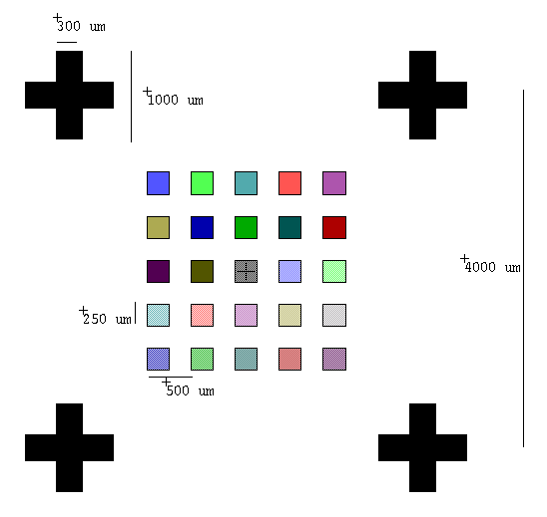
\includegraphics[scale=0.9]{Chapter-3/Figures/contrast_pattern.png}
 \caption[Computer-aided design for resist-contrast data collection]{CAD layout for resist-contrast data collection prepared using the \textsc{Tanner L-Edit} software package, where an array of \num{25} squares, each \SI{250}{\um} in width, is assigned to a range of values using \textsc{Layout BEAMER} \cite{McCoy18}.}\label{fig:dose_layout}
 \end{figure}
This pattern was exposed using a \SI{30}{\nano\ampere} beam current with a \SI{200}{\um} aperture in the \textsc{EBPG5200} to dose each square in \SI{7}{\percent} increments starting with $D = \SI{50}{\micro\coulomb\per\cm\squared}$ to impart a range of $M_w$ in the resist that correlates inversely with $D$. 
During wet development in MIBK/IPA, the resist in each square is etched at a rate that increases with decreasing $M_w$ to produce a different thickness of remaining resist \cite{miller-chou03}. 
These developed thicknesses were measured at the center of each square \SI{24}{\hour} post development using a focused \textsc{M-2000} ellipsometer (\textsc{J.A.\ Woollam}) installed at the Penn State Nanofabrication Laboratory \cite{PSU_MRI_nanofab}. 
To model the gathered data using \textsc{Woollam}'s \textsc{CompleteEASE} software package \cite{complete_ease}, SE analysis was restricted to $\SI{450}{\nm} < \lambda < \SI{1000}{\nm}$, where the resist is approximately transparent. 
\begin{figure}
 \centering
 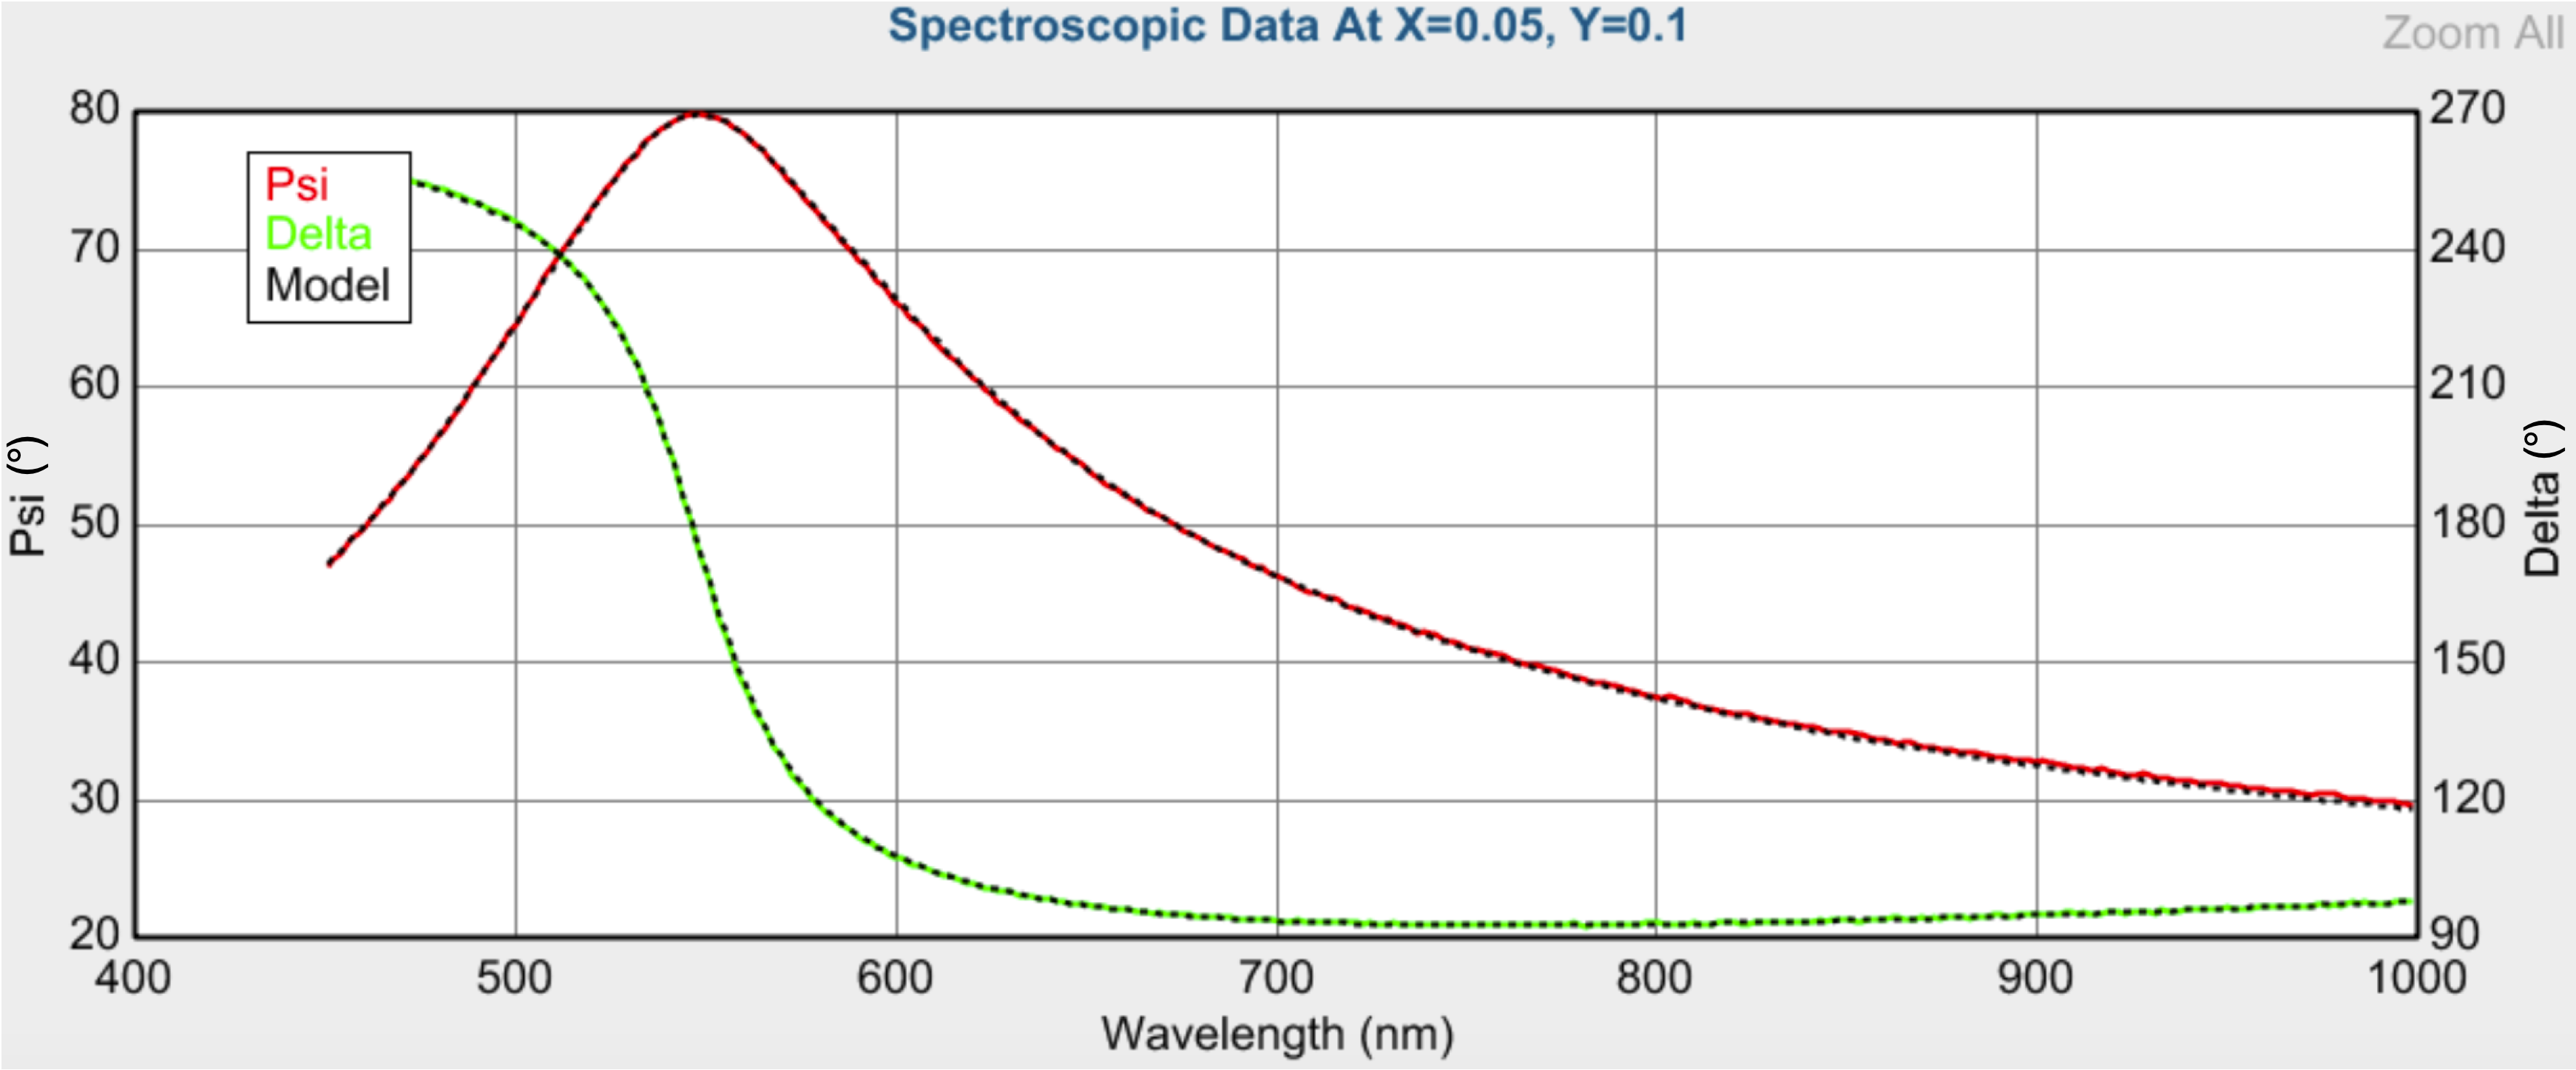
\includegraphics[scale=0.12]{Chapter-3/Figures/SE_data_example_fix.png}
 \includegraphics[scale=1.2]{Chapter-3/Figures/diffraction_arc28.mps}
 \caption[Example of a resist thickness measurement using SE]{Example of a resist thickness measurement using SE with \textsc{Woollam}'s \textsc{CompleteEASE} software package, where $\Psi$ and $\Delta$ are shown as red and green curves with units given in degrees (\emph{top}). The sample is treated as a bilayer on a substrate, where a film of native oxide is included between the resist and the silicon substrate, where both films are assumed to be transparent (\emph{bottom}; layers re not drawn to scale.). Using \cref{eq:Cauchy_index} for $\nu_2$ and tabulated data in \textsc{CompleteEASE} for $\nu_3$ and $\tilde{\nu}_4$, the thickness of resist in each dose square ($\tau_2$) could be measured with a fixed value of $\tau_3 = \SI{1.5}{\nm}$ for the native-oxide layer.}\label{fig:SE_example}
 \end{figure}
The sample was treated as a bilayer on a substrate, to account for the native \ce{SiO2} on the silicon wafer, with a reflectivity coefficient being a generalization of \cref{eq:refl_coeff_example} \cite{Gibaud2009}: 
\begin{equation}\label{eq:refl_coeff_bilayer}
 \tilde{r} = \frac{\tilde{r}_{1,2} + \tilde{r}_{2,3} \mathrm{e}^{-2 i \tilde{k}_{y,2} \tau_2} + \tilde{r}_{3,4} \mathrm{e}^{-2 i \left( \tilde{k}_{y,2} \tau_2 + \tilde{k}_{y,3} \tau_3 \right)} + \tilde{r}_{1,2} \tilde{r}_{2,3} \tilde{r}_{3,4} \mathrm{e}^{-2 i \tilde{k}_{y,3} \tau_3} }{1 + \tilde{r}_{1,2} \tilde{r}_{2,3} \mathrm{e}^{-2 i \tilde{k}_{y,2} \tau_2} + \tilde{r}_{2,3} \tilde{r}_{3,4} \mathrm{e}^{-2 i \tilde{k}_{y,3} \tau_3} + \tilde{r}_{1,2} \tilde{r}_{3,4} \mathrm{e}^{-2 i \left( \tilde{k}_{y,2} \tau_2 + \tilde{k}_{y,3} \tau_3 \right)}} ,
 \end{equation}
where the subscripts \numlist{1;2;3;4} correspond to air, PMMA, \ce{SiO2} and the silicon substrate as in \cref{fig:SE_example} with $\tau_2$ and $\tau_3$ representing the thicknesses of the resist and native-oxide layers, respectively. 

As described in \cref{sec:x-ray_index}, the complex index of refraction, $\tilde{\nu} (\omega) \equiv \nu (\omega) + i \xi (\omega)$, is related to the \emph{atomic scattering factor} defined by \cref{eq:atomic_scattering_factor_reduced2}, $f^0 \left( \omega \right)$, which is valid for forward-scattering in the soft x-ray, and more generally, for radiation with $\lambda$ much larger than the \emph{Bohr radius}, $a_0 \approx \SI{0.05}{\nm}$ [\emph{cf.\@} \cref{sec:SXR_med}]: 
\begin{subequations}
\begin{equation}\label{eq:index_atomic1}
 \tilde{\nu}^2 (\omega) = 1 - 4 \pi c_0 r_e \mathcal{N}_a \frac{f^0 \left( \omega \right)}{\omega^2} , 
 \end{equation}
where $c_0$ is the speed of light, $r_e$ is the classical electron radius and $\mathcal{N}_a$ is the atomic density of the material. 
A material can be considered transparent to radiation if $\omega$ is far from atomic resonances so that, neglecting effects related to absorption described by $\xi (\omega)$ and the damping terms of $f^0 \left( \omega \right)$, \cref{eq:index_atomic1} can be written in terms of the real index, $\nu (\omega)$, as 
\begin{equation}\label{eq:index_atomic2}
 \nu^2 (\omega) - 1 =  4 \pi c_0 r_e \mathcal{N}_a \sum_s \frac{g_s}{\left( \omega_s^2 - \omega^2 \right)} ,
 \end{equation}
\end{subequations}
where $g_s$ is the oscillator strength for an atomic resonance frequency $\omega_s$ [\emph{cf.\@} \cref{sec:scattering_atoms}]. 
For small $\nu$ and $\omega \ll \omega_s$, \cref{eq:index_atomic2} can be expanded as a Taylor series, rearranged and expressed in terms of $\lambda$ to arrive at \emph{Cauchy's equation} for a transparent film \cite{Born80}:
\begin{equation}\label{eq:Cauchy_index}
 \nu \left( \lambda \right) = A + \frac{B}{\lambda^2} + \frac{C}{\lambda^4} + \dotsc ,
 \end{equation}
where $A$, $B$ and $C$ are coefficients that are to be determined. 
\begin{figure}
 \centering
 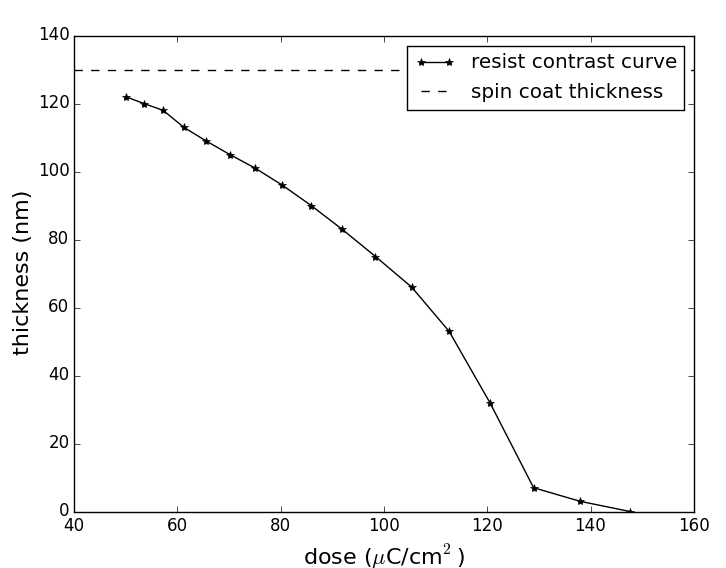
\includegraphics[scale=0.82]{Chapter-3/Figures/resist_contrast.png}
 \caption[Resist contrast for \SI{130}{\nm}-thick PMMA with $M_w = \SI{950}{\kilogram\per\mole}$]{Resist contrast for \SI{130}{\nm}-thick PMMA with $M_w = \SI{950}{\kilogram\per\mole}$ developed at room temperature using 1:1 MIBK/IPA for \SI{2}{\minute} and IPA for \SI{30}{\second}: the center of each square of the pattern shown in \cref{fig:dose_layout} is measured using spectroscopic ellipsometry and a film thickness is extracted. Resist contrast is plotted as remaining resist thickness as a function of electron dose, $D$ \cite{McCoy18}.}\label{fig:resist_contrast}
 \end{figure}
As $\nu$ is expected to change in each square of \cref{fig:dose_layout} due to electron exposure, $A$ and $B$ were fit using \textsc{Woollam}'s \textsc{CompleteEASE} software package \cite{complete_ease} for each measurement while keeping $C$ and all higher-order coefficients equal to zero. 
The native-oxide layer was accounted for as a \SI{1.5}{\nm}-thick film using tabulated data for $\nu$ provided in \textsc{CompleteEASE}; an example of such a measurement with both films is shown in \cref{fig:SE_example}. 
By repeating SE measurements for each of the \num{25} squares of \cref{fig:dose_layout}, resist thickness was extracted and plotted as a function of $D$ as a \emph{resist-contrast curve}, shown in \cref{fig:resist_contrast}, which served as the basis for GEBL in \SI{130}{\nm}-thick PMMA. 

\subsection[Test Patterns for Grayscale Electron-Beam Lithography]{Test Patterns for GEBL}\label{sec:GEBL}
%%%%%%%%%%%%%%%%%%%%%%%%%%%%%%%%%%%%%%%%%--------------------------------------------------
The standard approach employed for GEBL process development was to draw CAD for multi-level layouts that map design layer to intended resist thickness. 
Although a contrast curve gives remaining resist thickness as a function of electron dose by definition, \emph{proximity effect correction (PEC)} must be carried out to attain accurate GEBL structures as alluded to in \cref{sec:binary_ebeam} \cite{Pavkovich86}. 
This was handled using the \textsc{3DPEC} algorithm of \textsc{Layout BEAMER}, which uses input resist-contrast data and a point spread function for electron backscattering in silicon to calculate how dose is distributed for PEC \cite{beamer,Unal10}. %, determined through \emph{Monte Carlo simulation},\footnote{(very briefly explain this)}
The profile of energy distribution from electron scattering from an infinitesimally narrow source of current is described as a normalized sum of Gaussian distributions for forward-scattering in the resist and backscattering in the substrate with characteristic widths $\beta_f$ and $\beta_b$, respectively \cite{Pavkovich86}: 
\begin{align}
 \begin{split}
 f(\varrho) &= \frac{1}{1 + \eta_{\beta}} \left( \frac{1}{\pi \beta_f^2} \right) \mathrm{e}^{- \frac{\varrho^2}{\beta_f^2}} + \frac{\eta_{\beta}}{1 + \eta_{\beta}} \left( \frac{1}{\pi \beta_b^2} \right) \mathrm{e}^{- \frac{\varrho^2}{\beta_b^2}} \\
 &\approx \frac{1}{1 + \eta_{\beta}}  \left[ \delta_D (\varrho) + \frac{\eta_{\beta}}{\pi \beta_b^2} \mathrm{e}^{- \frac{\varrho^2}{\beta_b^2} } \right] ,
 \end{split}
 \end{align}
where $\varrho$ is a radial distance in the plane of the resist surface, $\eta_{\beta}$ is the ratio of deposited energy over $\beta_b$ to that of $\beta_f$. 
The approximation holds for small $\beta_f$ such that forward-scattering is treated as a Dirac delta function and backscattering in the substrate is entirely responsible for the proximity effect with $\beta_b \approx \SI{30}{\um}$ in a silicon wafer \cite{Pavkovich86,Czaplewski12}. 
By convolving this function with the incident current density of the electron beam, the energy deposited in the resist from backscattering can be inferred with the aid of \textsc{Layout BEAMER} to produce a dose-corrected layout fractured into \num{100} layers; this is exported to \textsc{EBPG5200} machine format as \num{100} \emph{pattern-generator (PG) shapes}. 
Patterns exposed in this way used a \SI{1}{\nano\ampere} beam current, a \SI{200}{\um} aperture and a \SI{10}{\nm} beam step size. 

Due to the added overhead associated with switching between PG shapes, an alternative approach utilizing \textsc{EBPG5200} \emph{sequencing} was also pursued. 
Unique to \textsc{EBPG} systems, sequencing is a set of commands that defines a series of lines and beam jumps to be executed as a custom, subfield-sized PG shape. 
This shape can be patterned over an arbitrary area using an array of subfield-sized rectangles defined in CAD. 
\begin{figure}
 \centering
 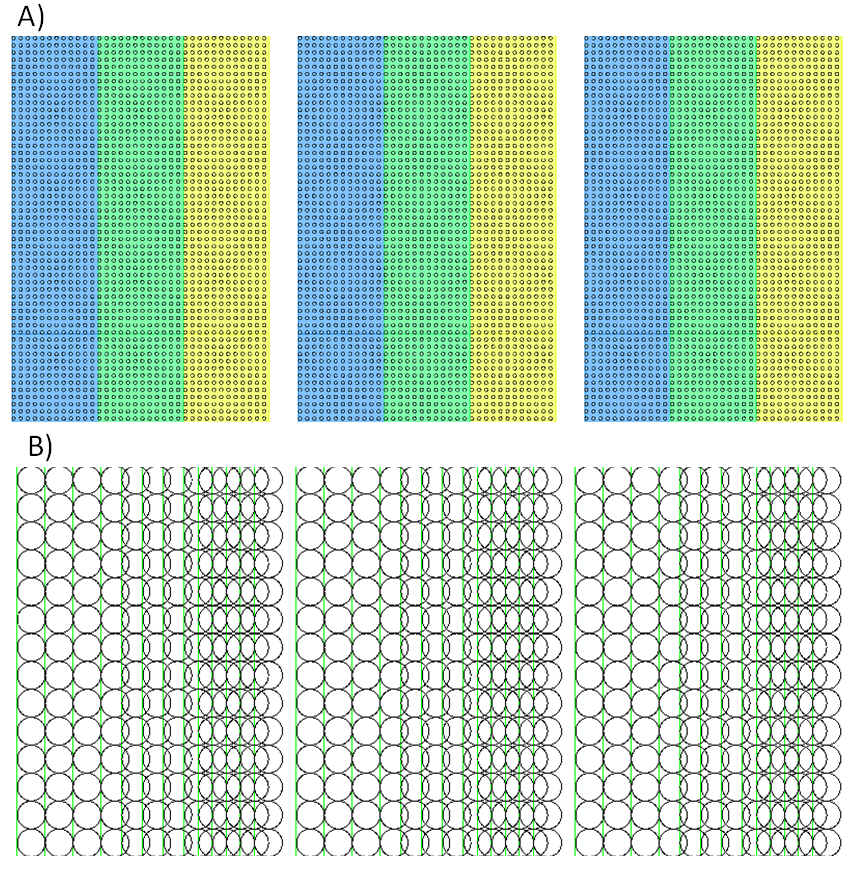
\includegraphics[scale=0.7]{Chapter-3/Figures/GEBL_approaches.png}
 \caption[\textsc{Layout BEAMER 3DPEC} and \textsc{EBPG5200} sequencing approaches to GEBL]{Two approaches to pattern generation for GEBL: a) Experimentally-determined data for resist contrast [\emph{cf.\@} \cref{fig:resist_contrast}] are input into \textsc{Layout BEAMER}, where the 3DPEC algorithm is used to generate a dose-corrected layout. Each dose is a different pattern generator (PG) shape, represented here with colorscale. b) Code for \textsc{EBPG5200} sequencing defines a custom subfield-sized pattern generator shape consisting of a series of lines and beam jumps using a fixed dose, where black circles represent \SI{40}{\nm}-diameter beam shots. Lines are programmed to overlap to varying degrees to emulate dose modulation achieved using the 3DPEC approach \cite{McCoy18}.}\label{fig:GEBL_approaches} 
 \end{figure}
Although sequencing is limited to lines and jumps at a single user-input value for $D$, dose modulation can be emulated using overlapping beams [\emph{cf.\@} \cref{fig:GEBL_approaches}]. 
In this way, GEBL patterns were produced by generating sequencing code for a \SI{4}{\um}-large custom PG shape to approximate the dose-corrected layout from 3DPEC. 
These patterns used a \SI{25}{\nano\ampere} beam current, a \SI{400}{\um} aperture and a \SI{40}{\nm} beam step size with the electron beam defocused to a \SI{40}{\nm} diameter. 
The input dose was determined through analysis of dose test arrays and the highest possible beam current\footnote{This beam current was limited by the \SI{25}{\mega\hertz} \textsc{EBPG5200} clock frequency at the time of the experiment (2017) \cite{McCoy18}.} was used to write each pattern. 

Using these two GEBL approaches, multi-level staircase structures with \SI{840}{\nm} and \SI{400}{\nm} periodicities were patterned in PMMA resist. 
The width of staircase steps generally were designed to be comparable to the nominal spin-coat thickness of \SI{130}{\nm}. 
A series of GEBL test samples were written over \SI{0.5}{\mm} by \SI{2}{\mm} areas featuring the following patterns:
\begin{itemize}[noitemsep] 
 \item \emph{pattern A}: 6-level staircase where each step is \SI{140}{\nm} wide to give $d = \SI{840}{\nm}$
 \item \emph{pattern B}: 4-level staircase where each step is \SI{100}{\nm} wide to give $d = \SI{400}{\nm}$
 \item \emph{pattern C}: 4-level staircase where the width of the top step is reduced to \SI{40}{\nm}; remaining levels are \SI{120}{\nm} wide to give $d = \SI{400}{\nm}$
 \item \emph{pattern D}: Emulation of pattern C attained through \textsc{EBPG5200} sequencing\footnote{This was carried out according to the pattern shown in \cref{fig:GEBL_approaches}(B), where the overlapping beams emulate doses $D$, $1.5D$ and $2D$ with $D = \SI{75}{\micro\coulomb\per\cm\squared}$ as the user-input dose.}
 \end{itemize}%
As described at the start of \cref{sec:TASTE}, the staircase steps intermediate between the top step and the exposed substrate will, in principle, equilibrate into sloped surfaces with application of an optimized thermal treatment \cite{Schleunitz11a,Schleunitz14}. 
The width of the top step in patterns C and D was reduced in an effort to minimize flat area atop groove structures in the final product. 
Ideally, grooves are sharp, triangular sawtooth facets to provide an effective blazed grating response. 

Untreated GEBL structures in PMMA for patterns A-D are shown under AFM in \cref{fig:GEBL_ABCD}.  
\begin{figure}
 \centering
 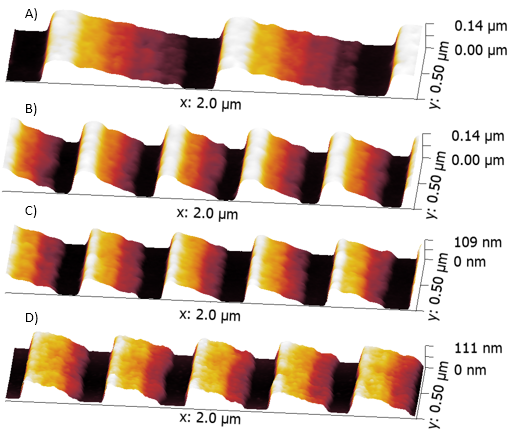
\includegraphics[scale=1.2]{Chapter-3/Figures/GEBL.png}
 \caption[GEBL test patterns in \SI{130}{\nm}-thick PMMA examined under AFM]{GEBL in \SI{130}{\nm}-thick PMMA examined under AFM. Patterns A-C were attained through the standard 3DPEC approach while pattern D is a result from the \textsc{EBPG5200} sequencing approach: a) Pattern A: GEBL with 6 levels where each are \SI{140}{\nm} wide to give a \SI{840}{\nm} periodicity, b) Pattern B: GEBL with 4 levels where each are \SI{100}{\nm} wide to give a \SI{400}{\nm} periodicity, c) Pattern C: GEBL with 4 levels where the width of the top level is reduced to \SI{40}{\nm}; remaining levels are \SI{120}{\nm} wide to give a periodicity of \SI{400}{\nm}, d) Pattern D: same as pattern C but attained using EBPG sequencing \cite{McCoy18}.}\label{fig:GEBL_ABCD}
 \end{figure}
Using \textsc{Bruker}'s \textsc{PeakForce Tapping}$^{\text{TM}}$ mode \cite{Xu18}, patterns were scanned over \SI{2}{\um} at \num{512} samples per line to give a \SI{3.9}{\nm} AFM pixel size. 
In patterns A and B, staircase steps are equal in width and the overall structure height is comparable to the initial spin-coat thickness as measured by AFM. 
However, due to the narrowed width of the top step in patterns C and D, which is the same size as the defocused electron-beam diameter, the overall structure height is reduced to about \SI{75}{\percent} of the original film thickness achieved by spin coating. 
Patterns A-C were fabricated using the \textsc{Layout BEAMER 3DPEC} approach, where a \SI{1}{\mm\squared} area is exposed in $\sim \SI{20}{\minute}$ using the EBPG5200. 
In contrast, pattern D over the same area can be written using \textsc{EBPG5200} sequencing in $\sim \SI{1}{\minute}$. 
Although pattern D exhibits higher noise than pattern C under AFM, the end result should be comparable owing to the smoothing effect of thermal reflow. 
%after thermal reflow should be comparable. 
For this reason, the \textsc{EBPG5200} sequencing approach is expected to be valuable for patterning by GEBL over large areas. 

\subsection{Selective Thermal Reflow}\label{sec:reflow_results} 
%%%%%%%%%%%%%%%%%%%%%%%%%%%%%%%%%%%%%%%%%--------------------------------------------------
To induce selective thermal reflow in the GEBL test patterns [\emph{cf.\@} \cref{fig:GEBL_ABCD}] such that the top, unexposed staircase step remains largely unaffected, the resist must be heated at an appropriate temperature, $T = T_{\text{reflow}}$, for a duration, $t$, that is long enough to allow the exposed staircase steps to equilibrate into a wedge-like, smooth surface as has been shown previously for \si{\um}-scale GEBL patterns \cite{Schleunitz10,Schleunitz11a,Schleunitz14,Kirchner19}. 
All thermal reflow experimentation to probe this parameter space for the smaller-scale patterns considered was carried out using an automated hotplate on a resist stabilization system built by \textsc{Fusion Semiconductor} at the Penn State Nanofabrication Laboratory \cite{PSU_MRI_nanofab}. 
The tool, which accepts wafers with \SI{100}{\mm} and \SI{150}{\mm} diameters, was employed for heating test samples in a controllable and reproducible way. 
A series of identical GEBL samples were fabricated and thermally treated under different conditions to probe the $T$-$t$ parameter space for TASTE. 
Using a short heating duration ($t = \SI{20}{\second}$), samples were treated using a range of $T$ around the expected $T_{\text{reflow}}$ for PMMA (\SIrange{110}{130}{\celsius}). 
Conversely, samples were heated for different values of $t$, (\SIlist{20;60;120}{\second}) while holding $T$ constant at \SI{120}{\celsius}. 
Each sample was allowed to cool on the cassette rack of the automated hotplate tool after heating.

Thermal-reflow test results for pattern A as a function of $T$ and $t$ are shown in \cref{fig:A_temp_scan,fig:A_time_scan}, respectively. 
\begin{figure}
 \centering
 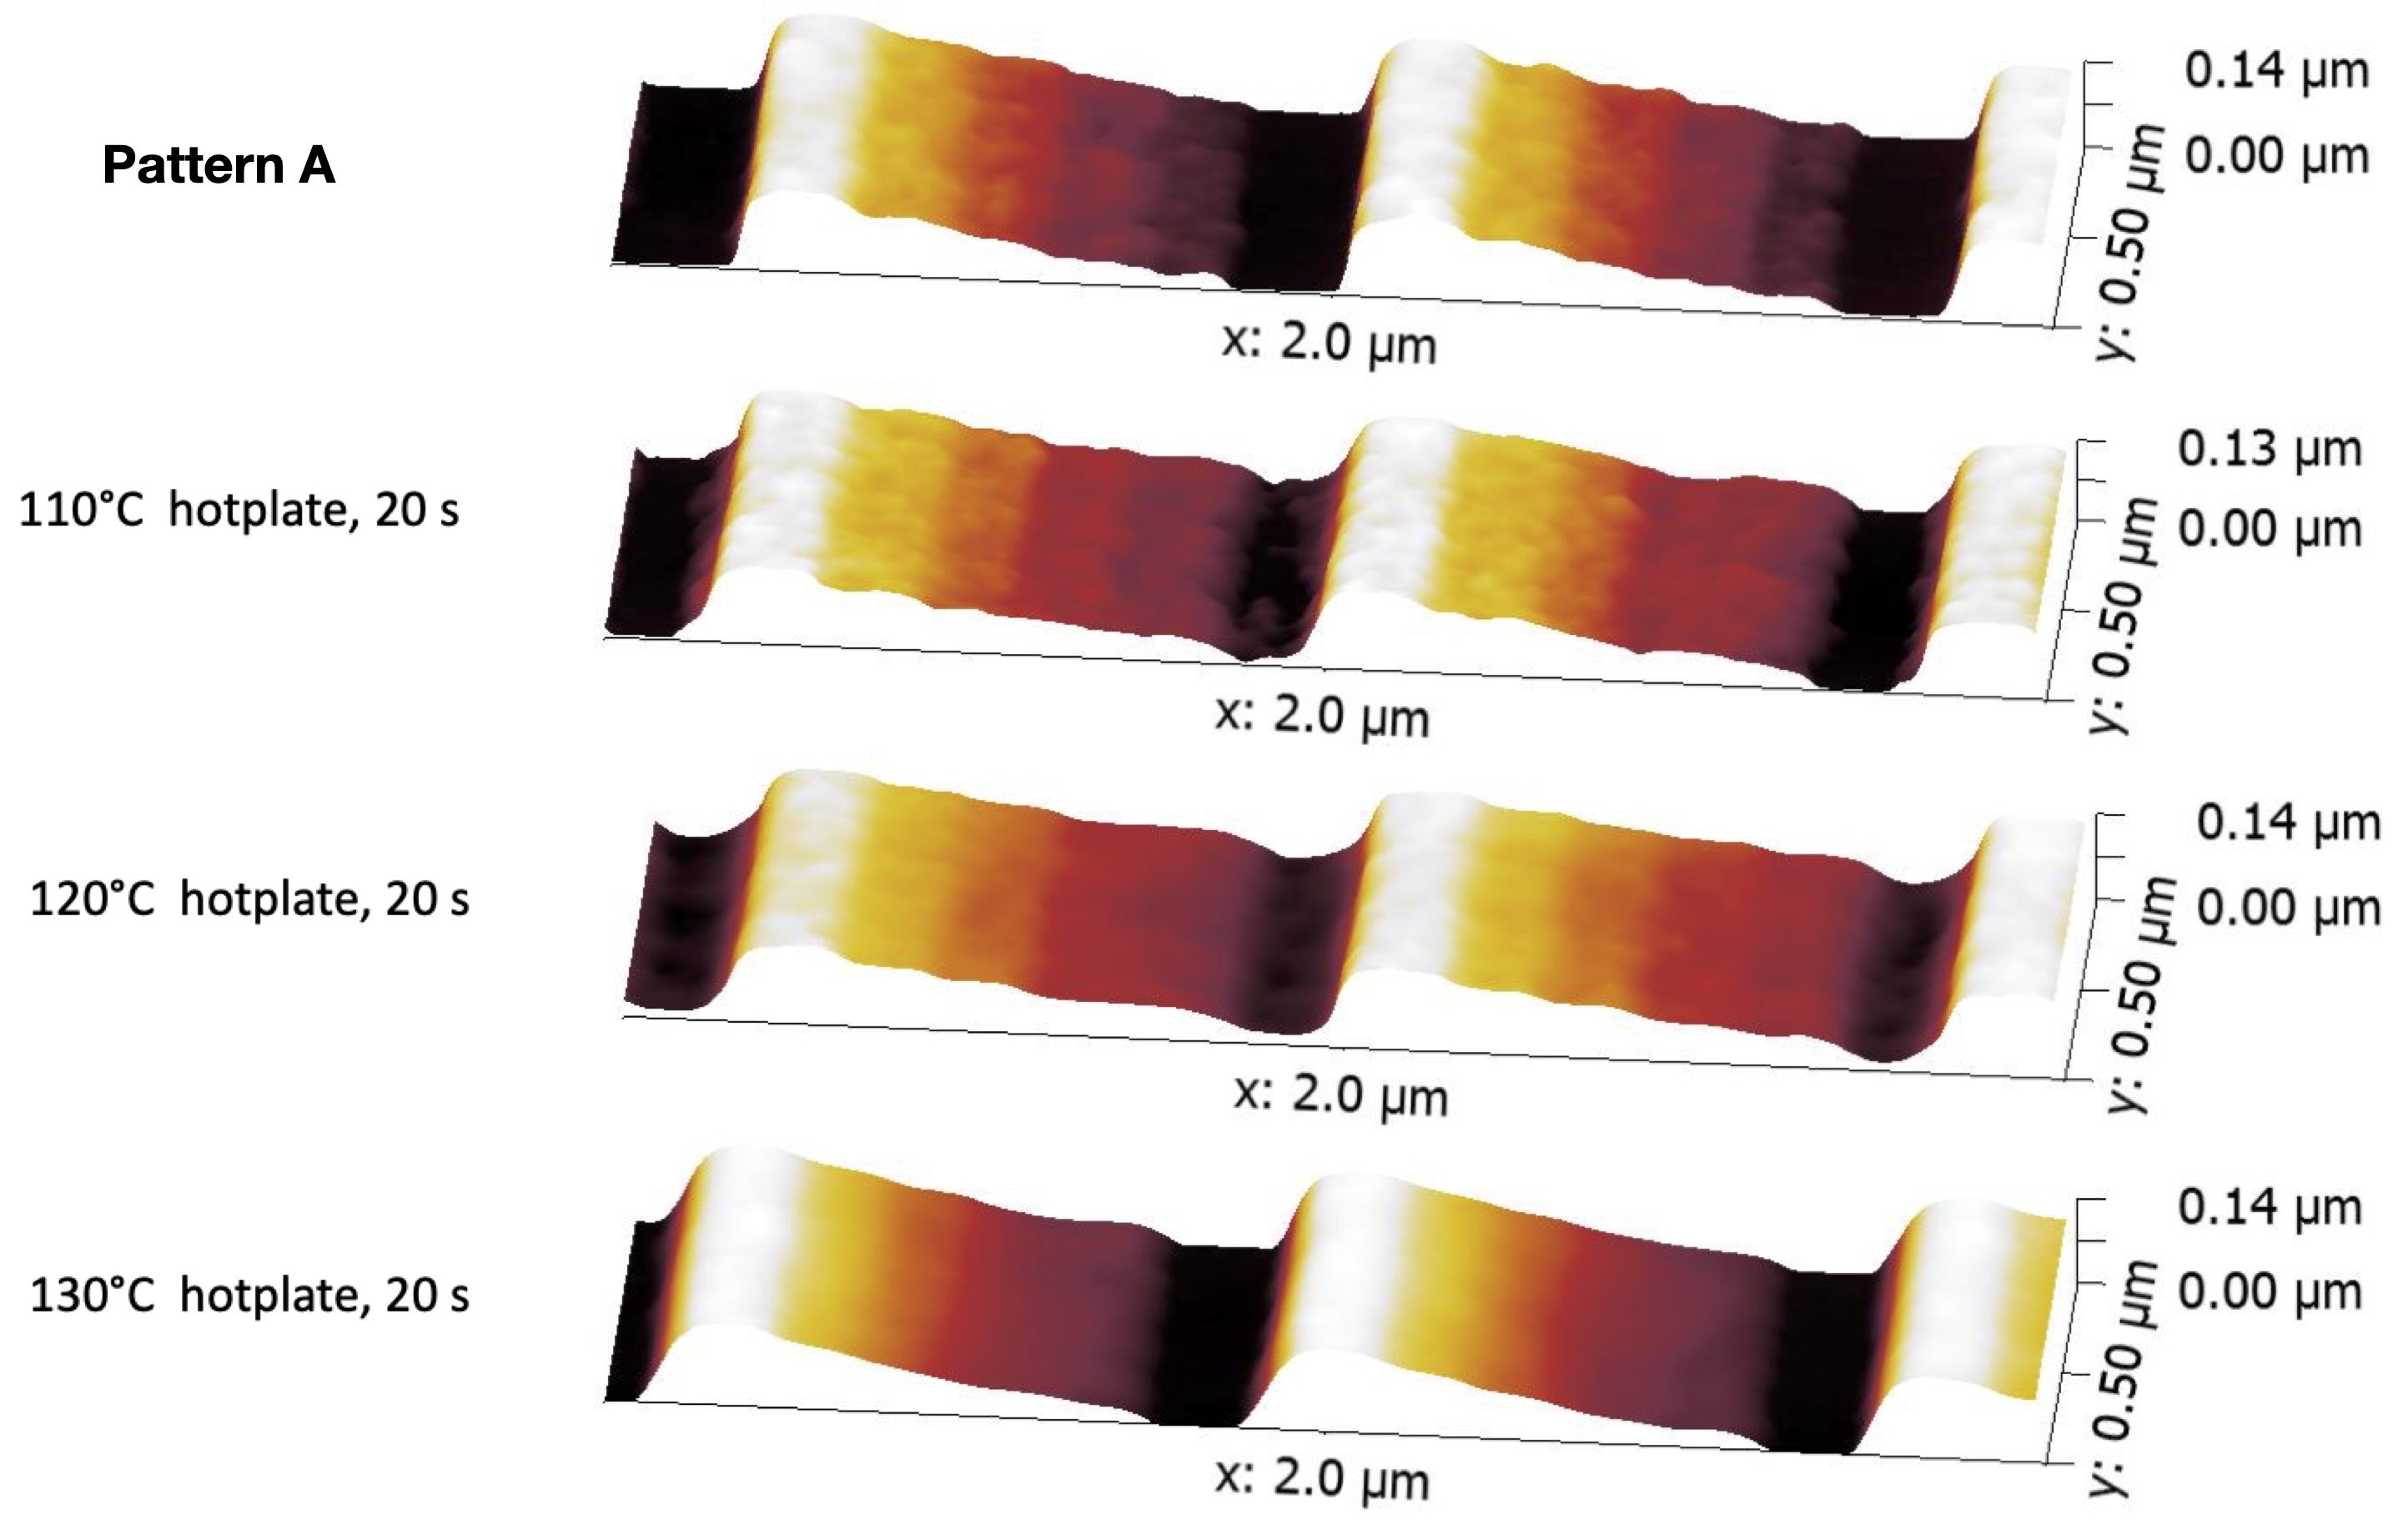
\includegraphics[scale=0.1505]{Chapter-3/Figures/A_temp_scan.jpg}
 \caption[Thermal reflow results as a function of heating temperature for grayscale pattern A]{Thermal reflow results as a function of heating temperature, $T$, for GEBL in \SI{130}{\nm}-thick PMMA with \num{6} levels: each are \SI{140}{\nm} wide to give $d = \SI{840}{\nm}$ \cite{McCoy18}.}\label{fig:A_temp_scan}
 \end{figure}
\begin{figure}
 \centering
 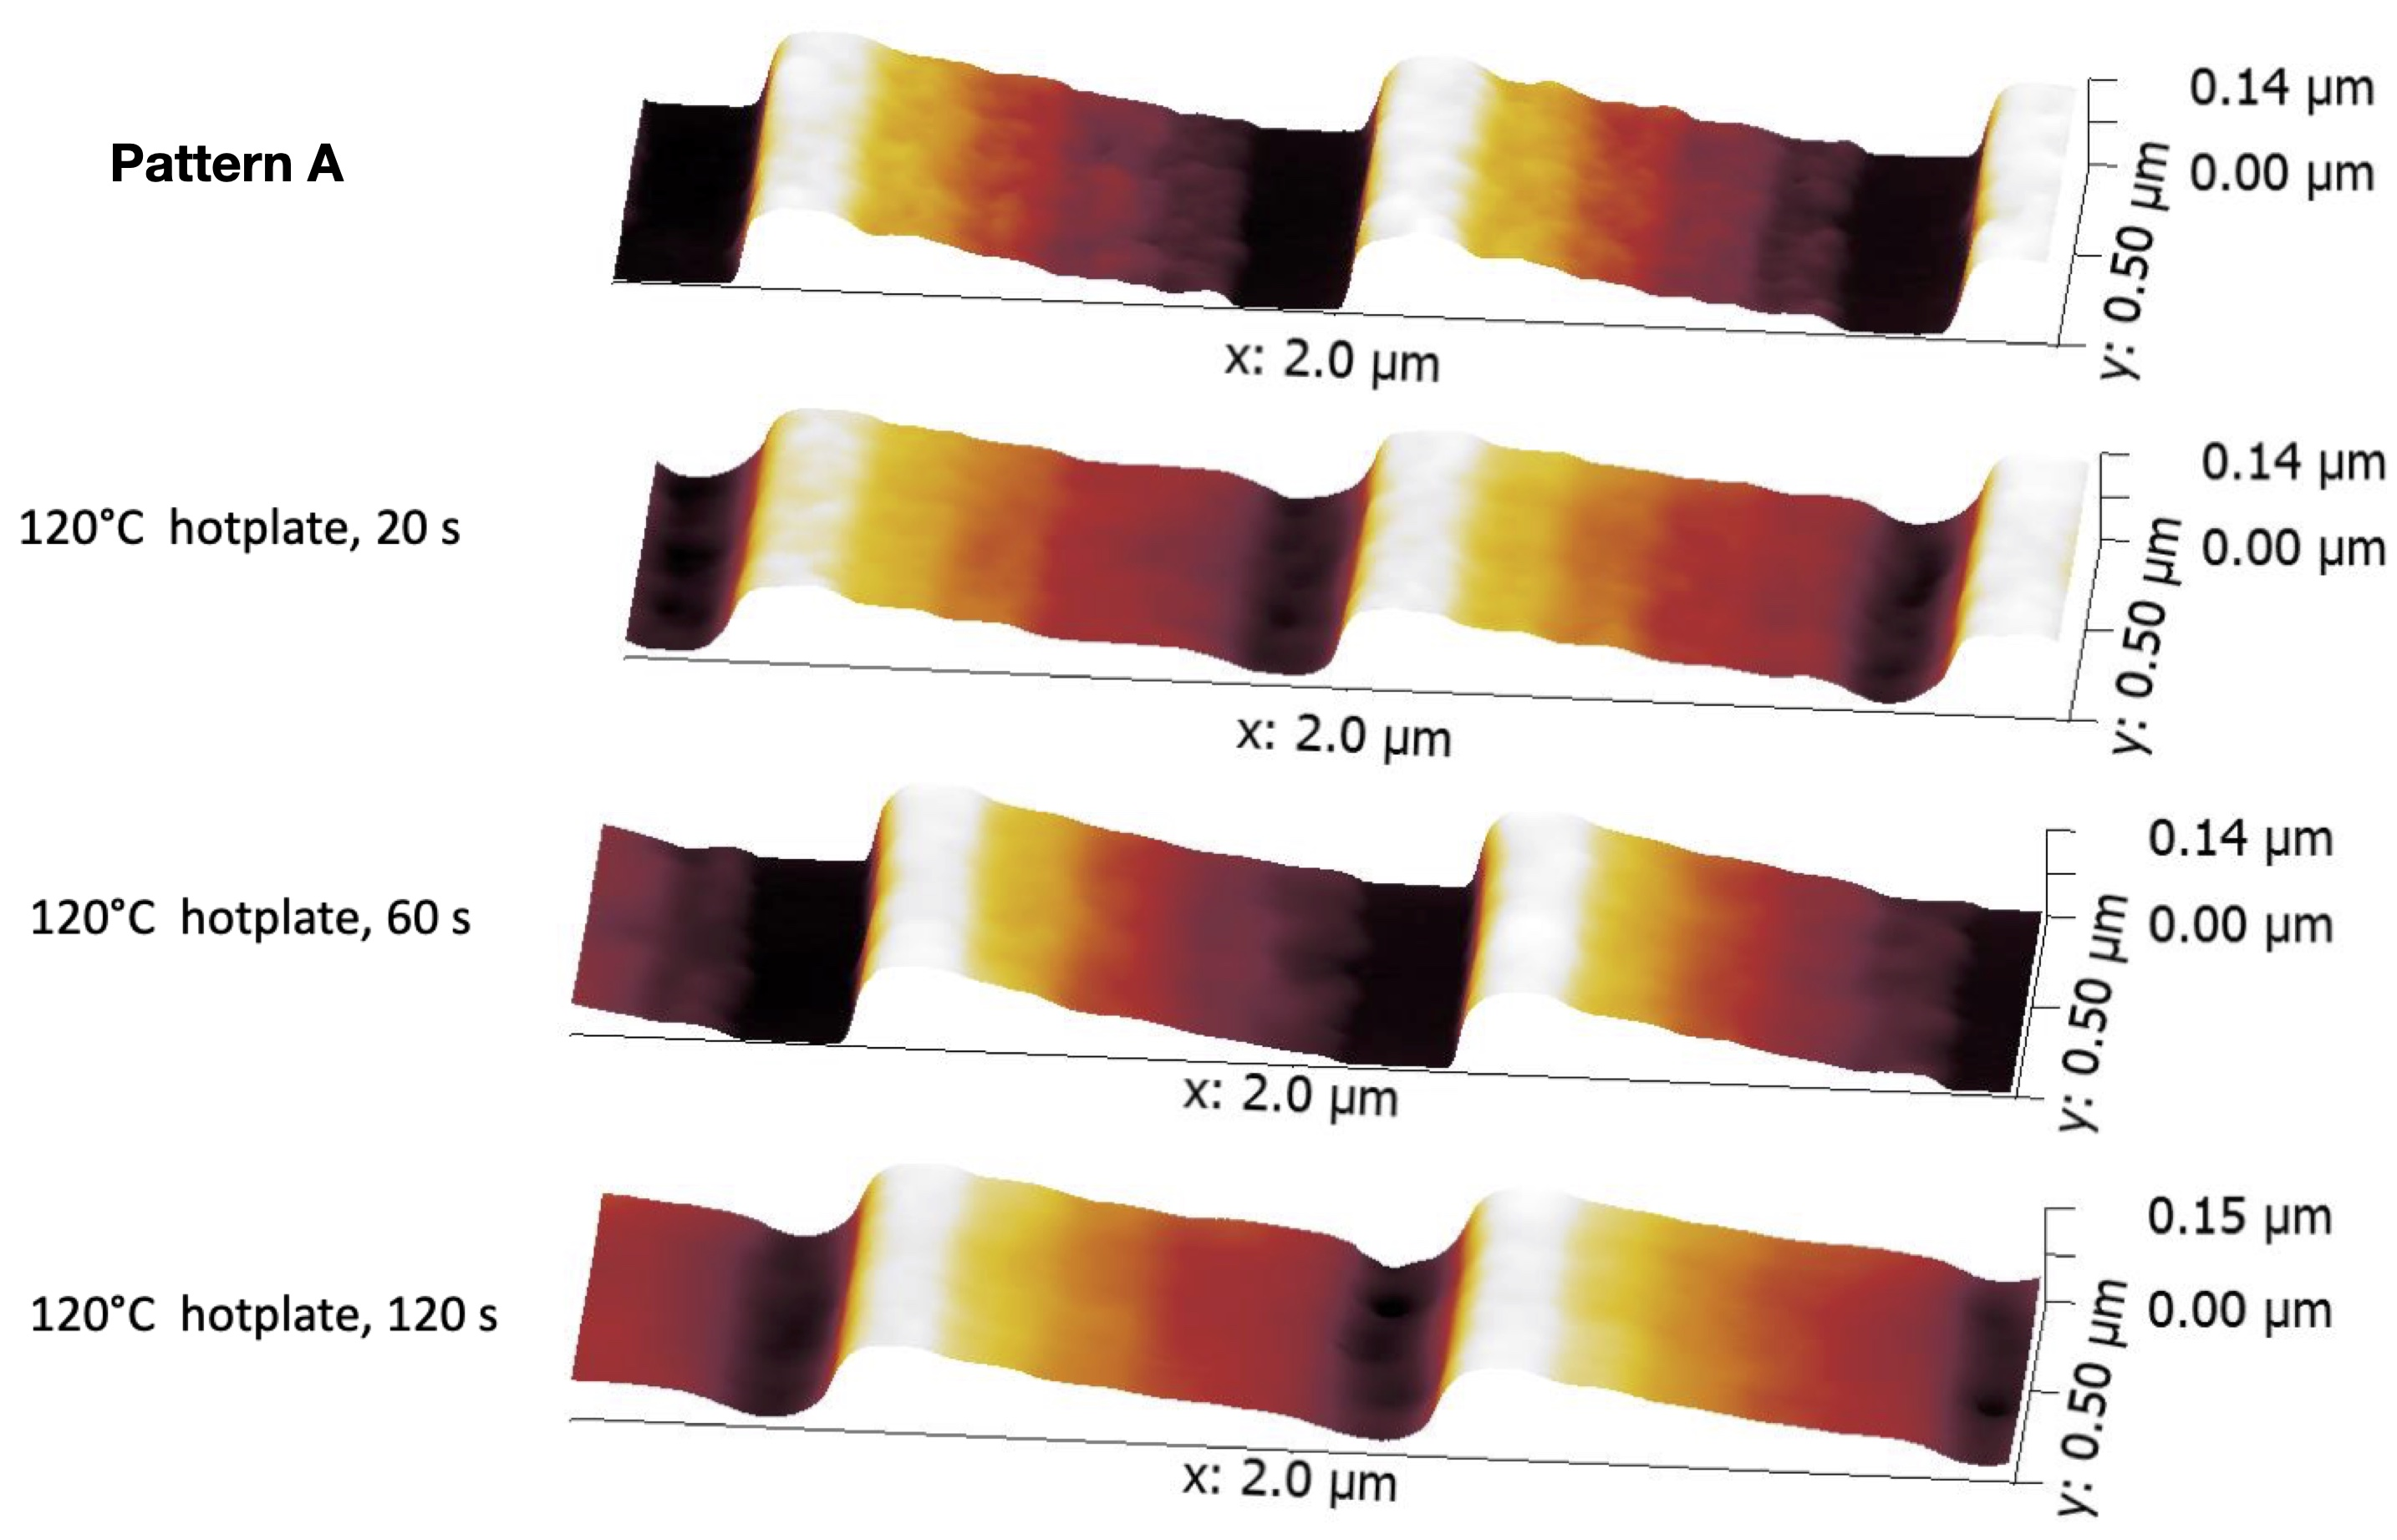
\includegraphics[scale=0.1505]{Chapter-3/Figures/A_time_scan.jpg}
 \caption[Thermal reflow results as a function of heating duration for grayscale pattern A]{Thermal reflow results as a function of heating duration, $t$, for GEBL in \SI{130}{\nm}-thick PMMA with \num{6} levels as in \cref{fig:A_temp_scan} \cite{McCoy18}.}\label{fig:A_time_scan}
 \end{figure}
Together, these include six AFM scans: three samples treated at \SIlist{110;120;130}{\celsius} keeping heating time constant at \SI{20}{\second}, and, three samples heated with durations of \SIlist{20;60;120}{\second} holding temperature at \SI{120}{\celsius}. 
Analogous AFM scans of thermal reflow results are shown in \cref{fig:B_temp_scan,fig:B_time_scan} for pattern B and in \cref{fig:C_temp_scan,fig:C_time_scan} for pattern C \cite{McCoy18}.
\begin{figure}
 \centering
 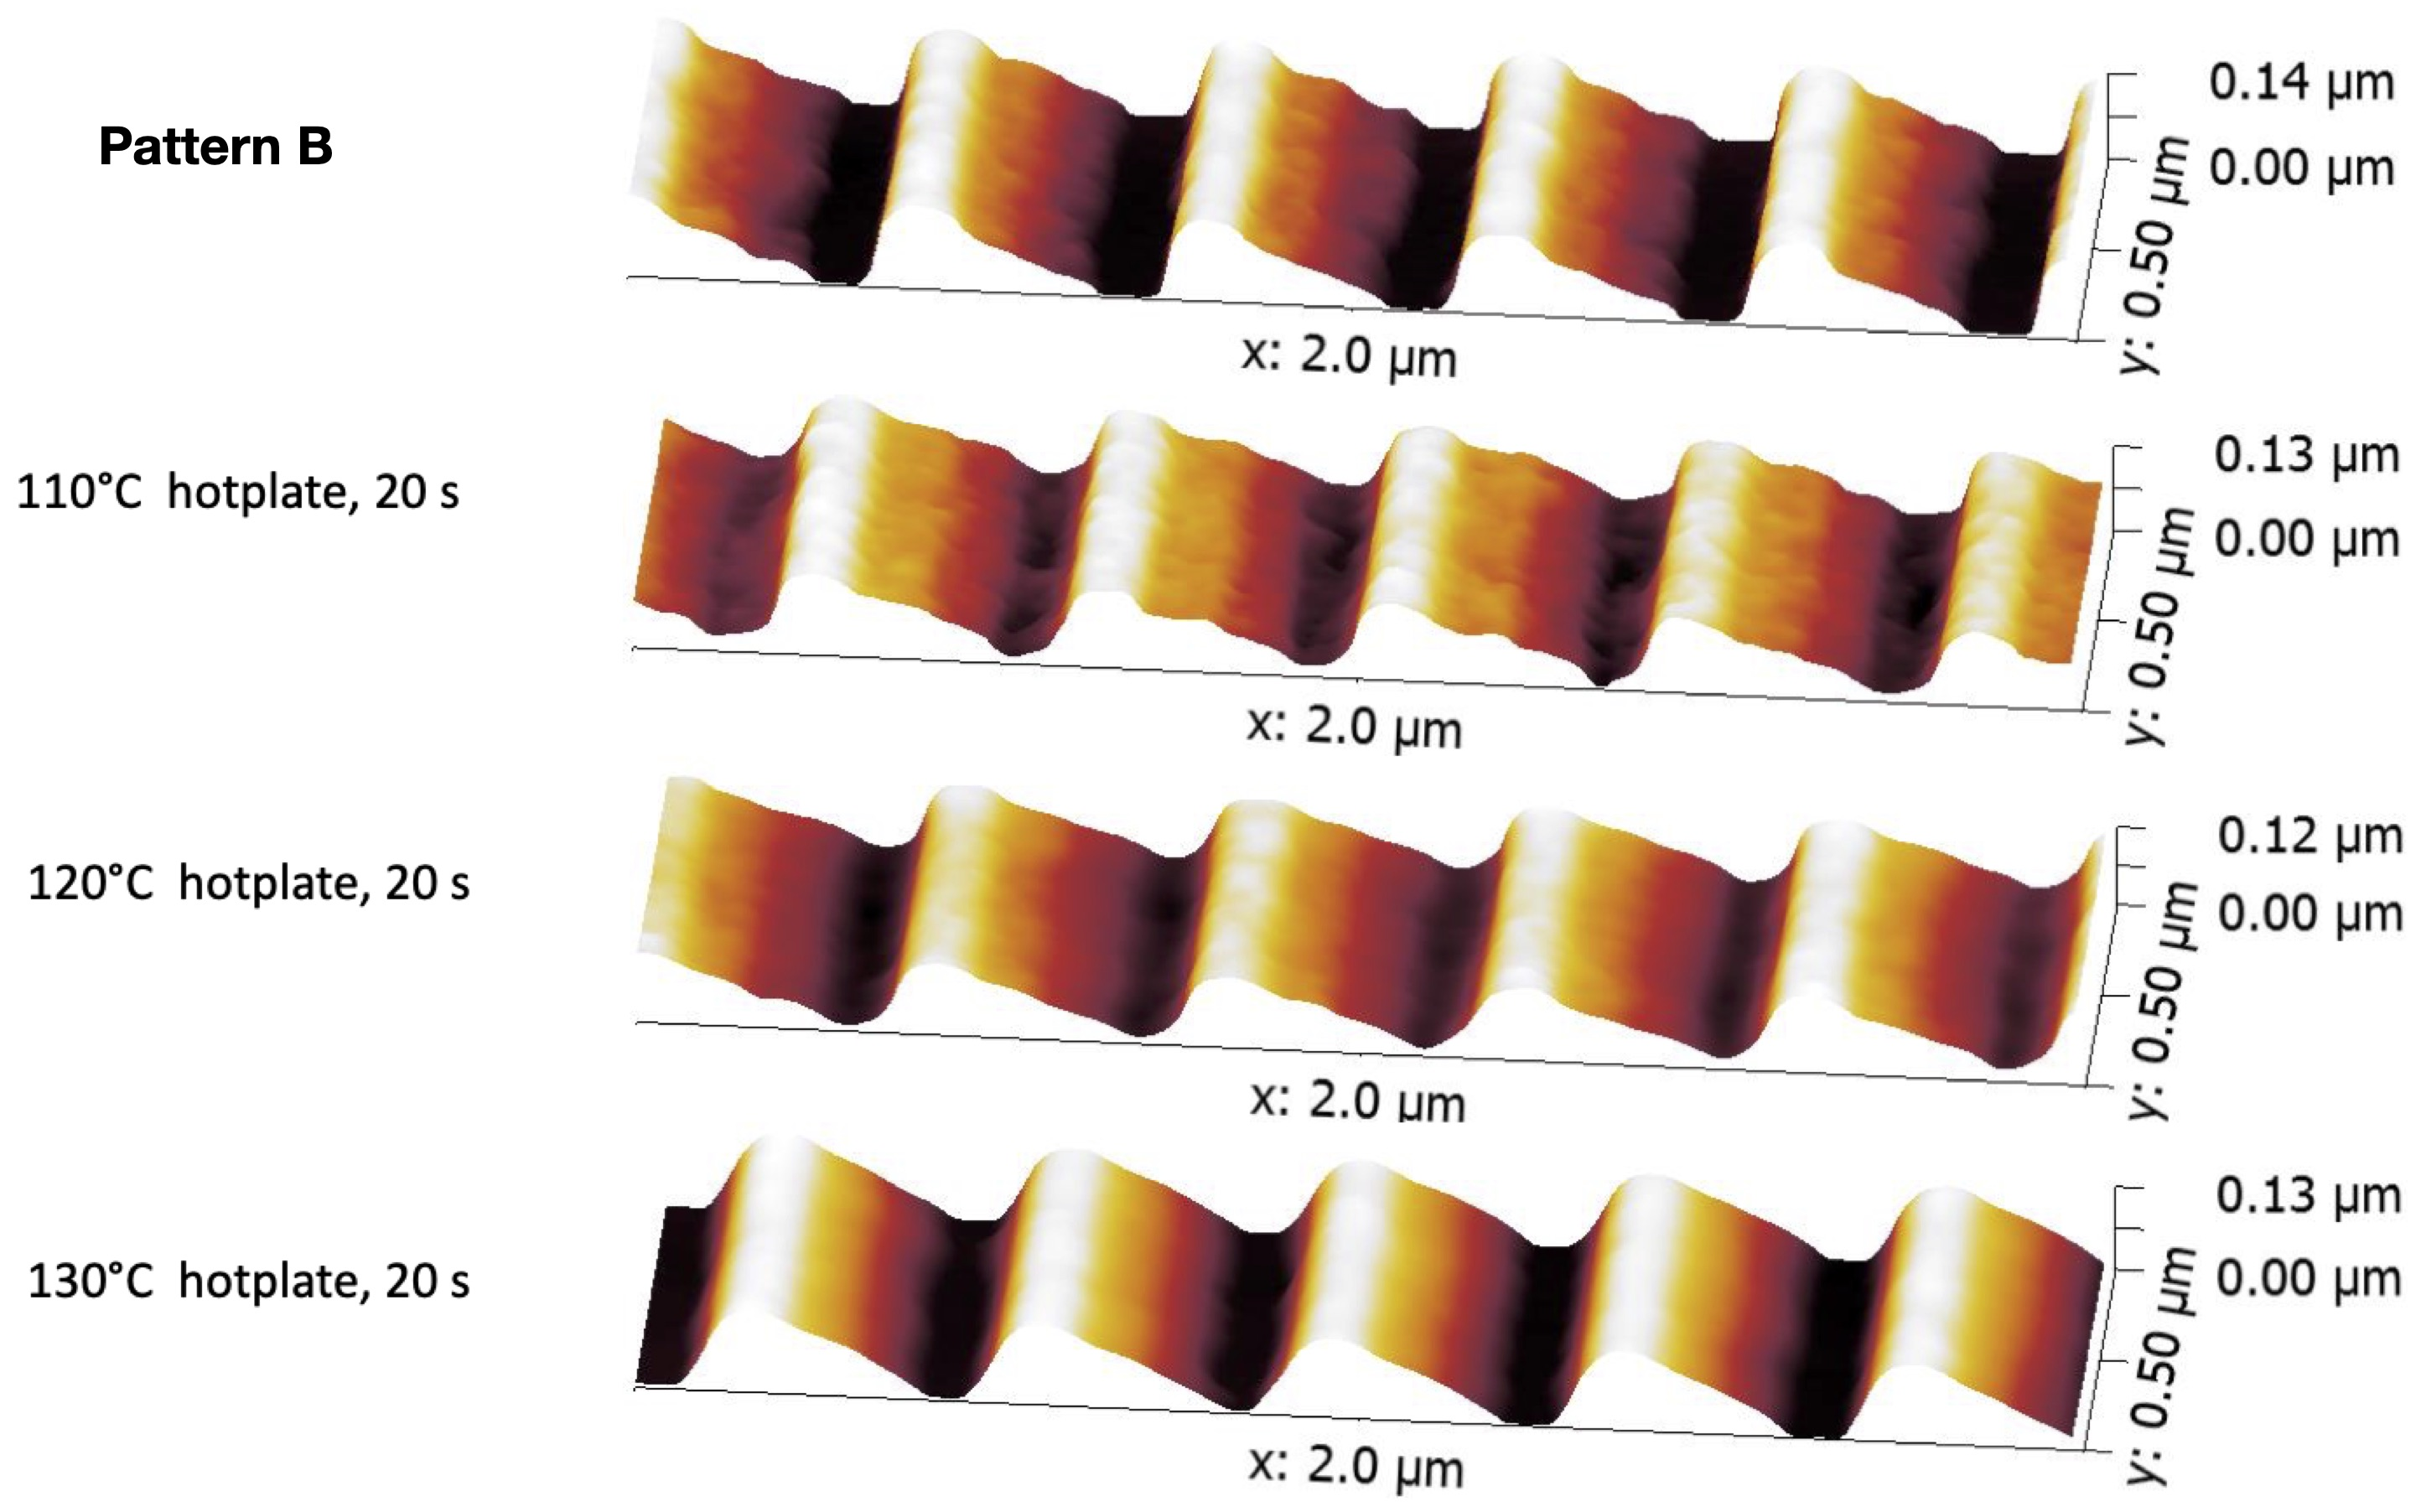
\includegraphics[scale=0.1505]{Chapter-3/Figures/B_temp_scan.jpg}
 \caption[Thermal reflow results as a function of heating temperature for grayscale pattern B]{Thermal reflow results as a function of $T$ for GEBL in \SI{130}{\nm}-thick PMMA with \num{4} levels: each are \SI{100}{\nm} wide to give $d = \SI{400}{\nm}$ \cite{McCoy18}.}\label{fig:B_temp_scan}
 \end{figure}
\begin{figure}
 \centering
 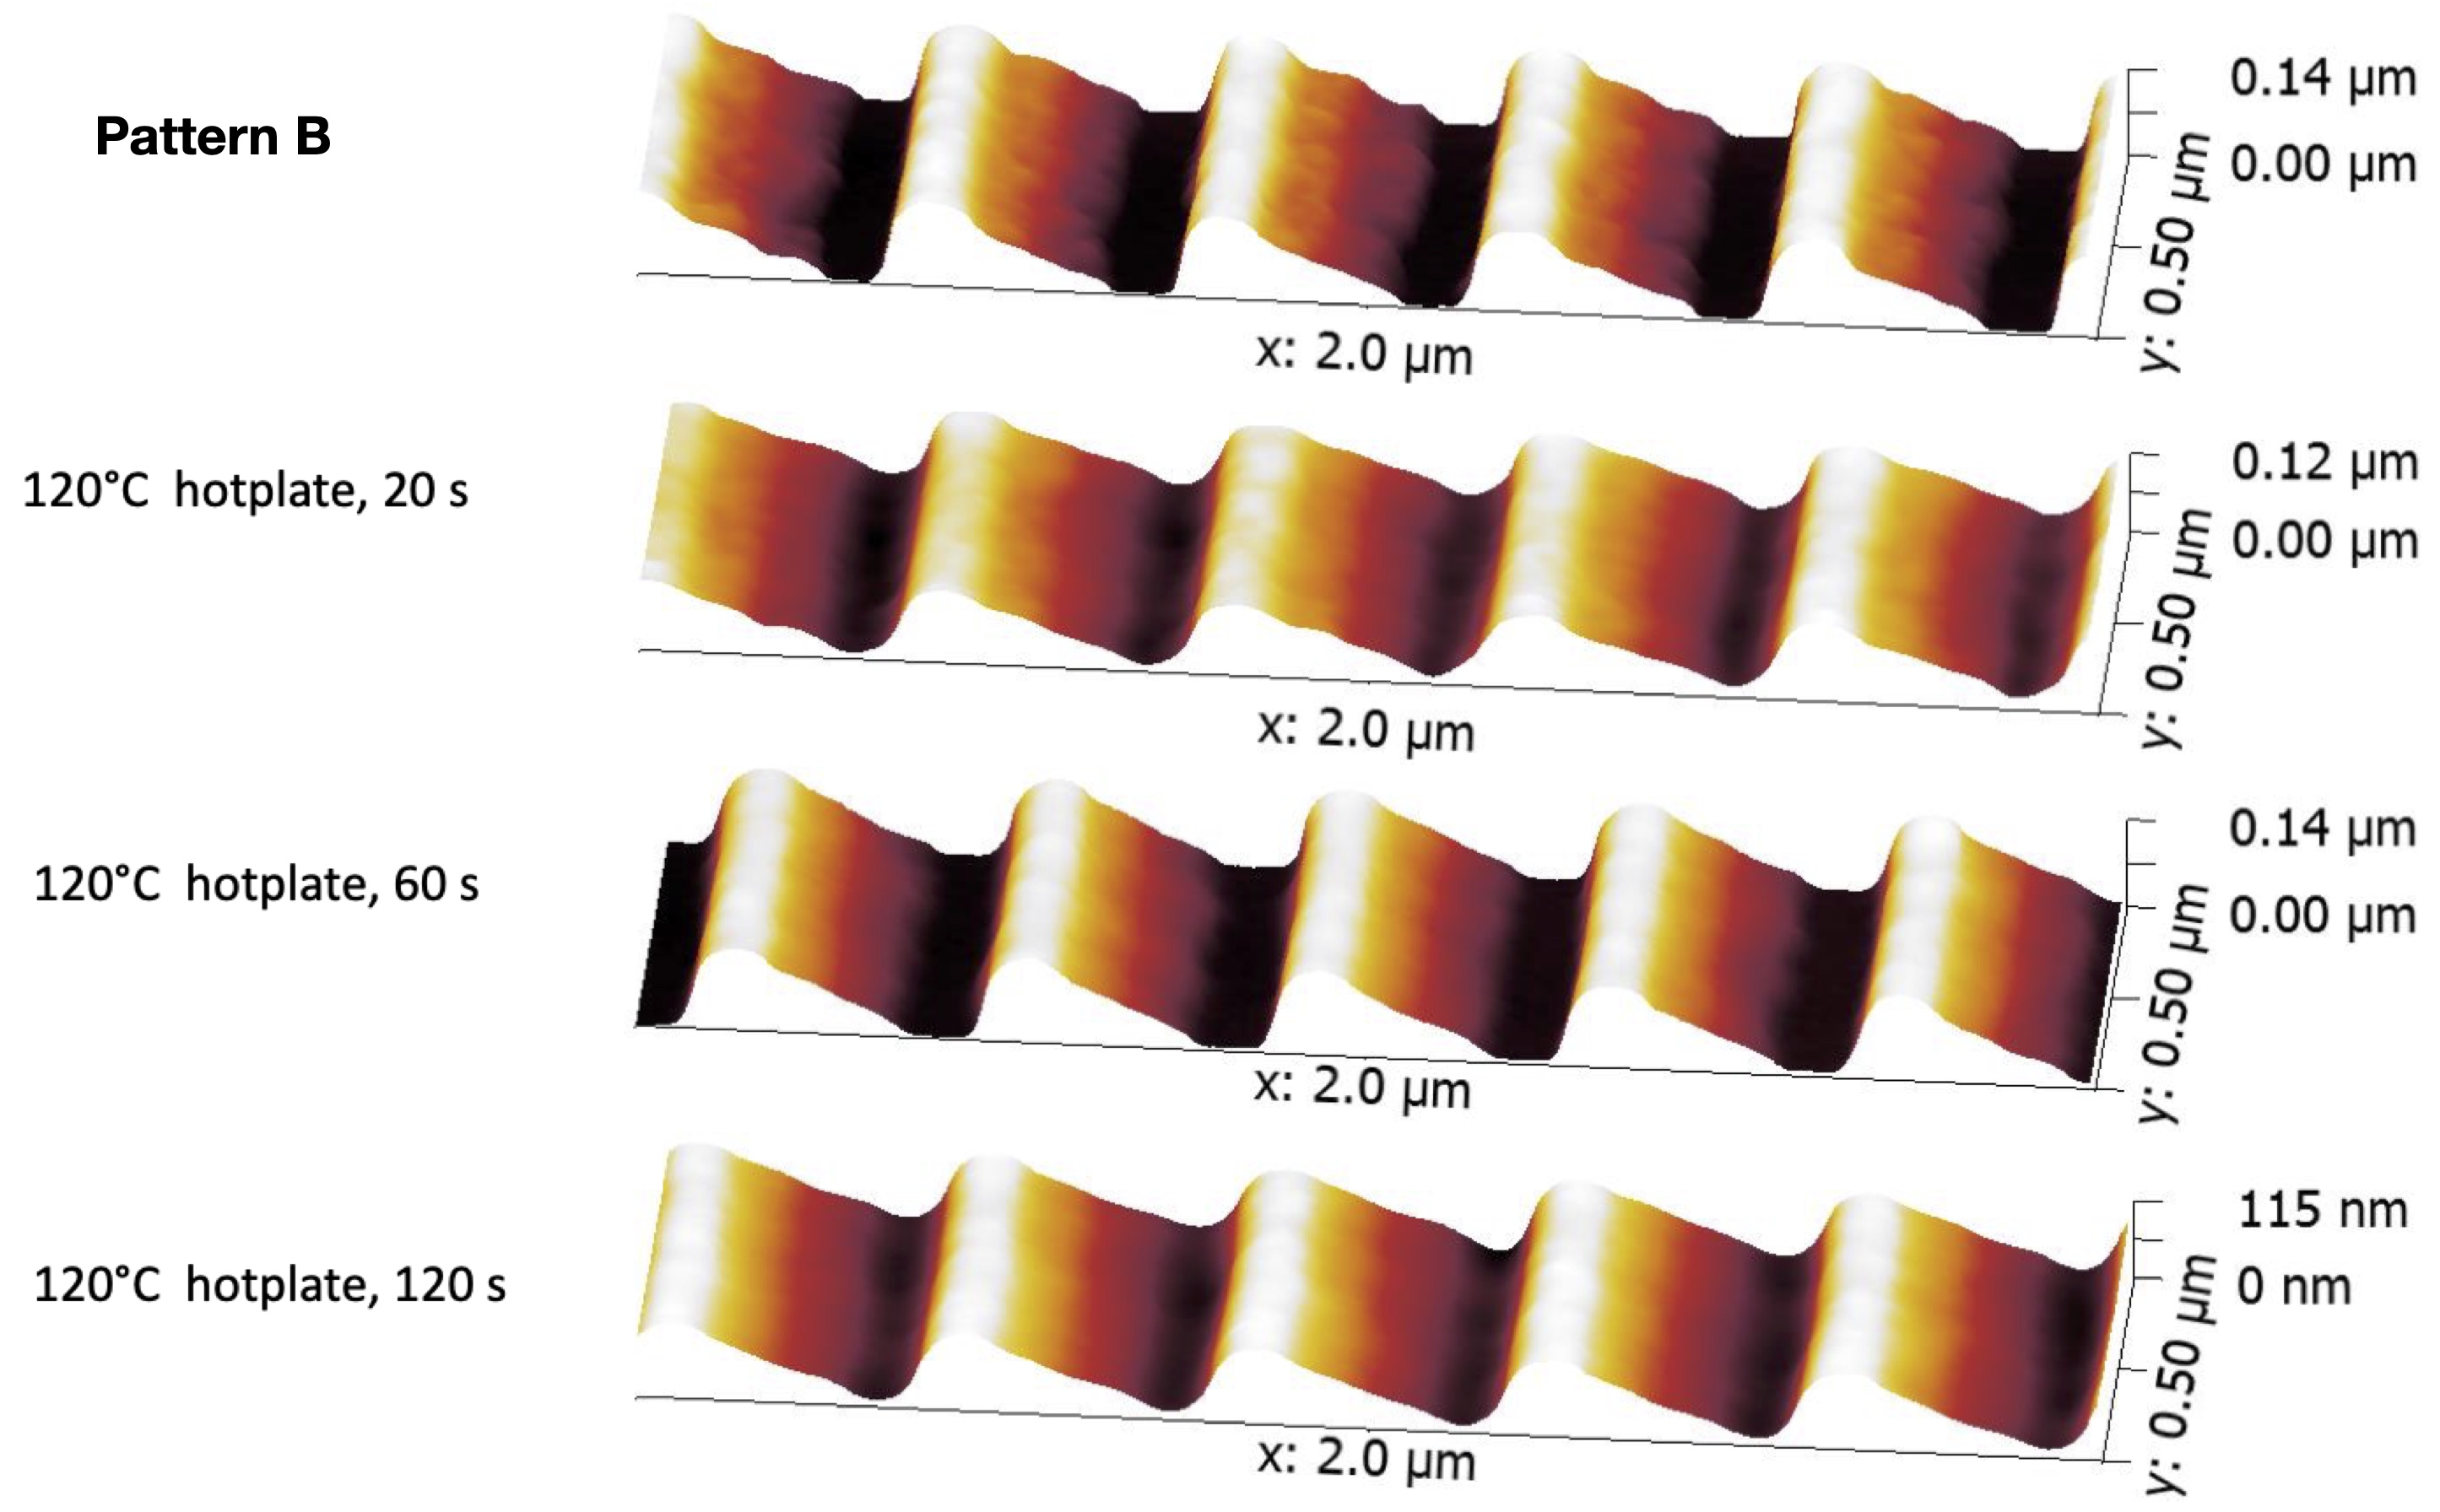
\includegraphics[scale=0.1505]{Chapter-3/Figures/B_time_scan.jpg}
 \caption[Thermal reflow results as a function of heating duration for grayscale pattern B]{Thermal reflow results as a function of $t$ for GEBL in \SI{130}{\nm}-thick PMMA with \num{4} levels as in \cref{fig:B_temp_scan} \cite{McCoy18}.}\label{fig:B_time_scan}
 \end{figure}
\begin{figure}
 \centering
 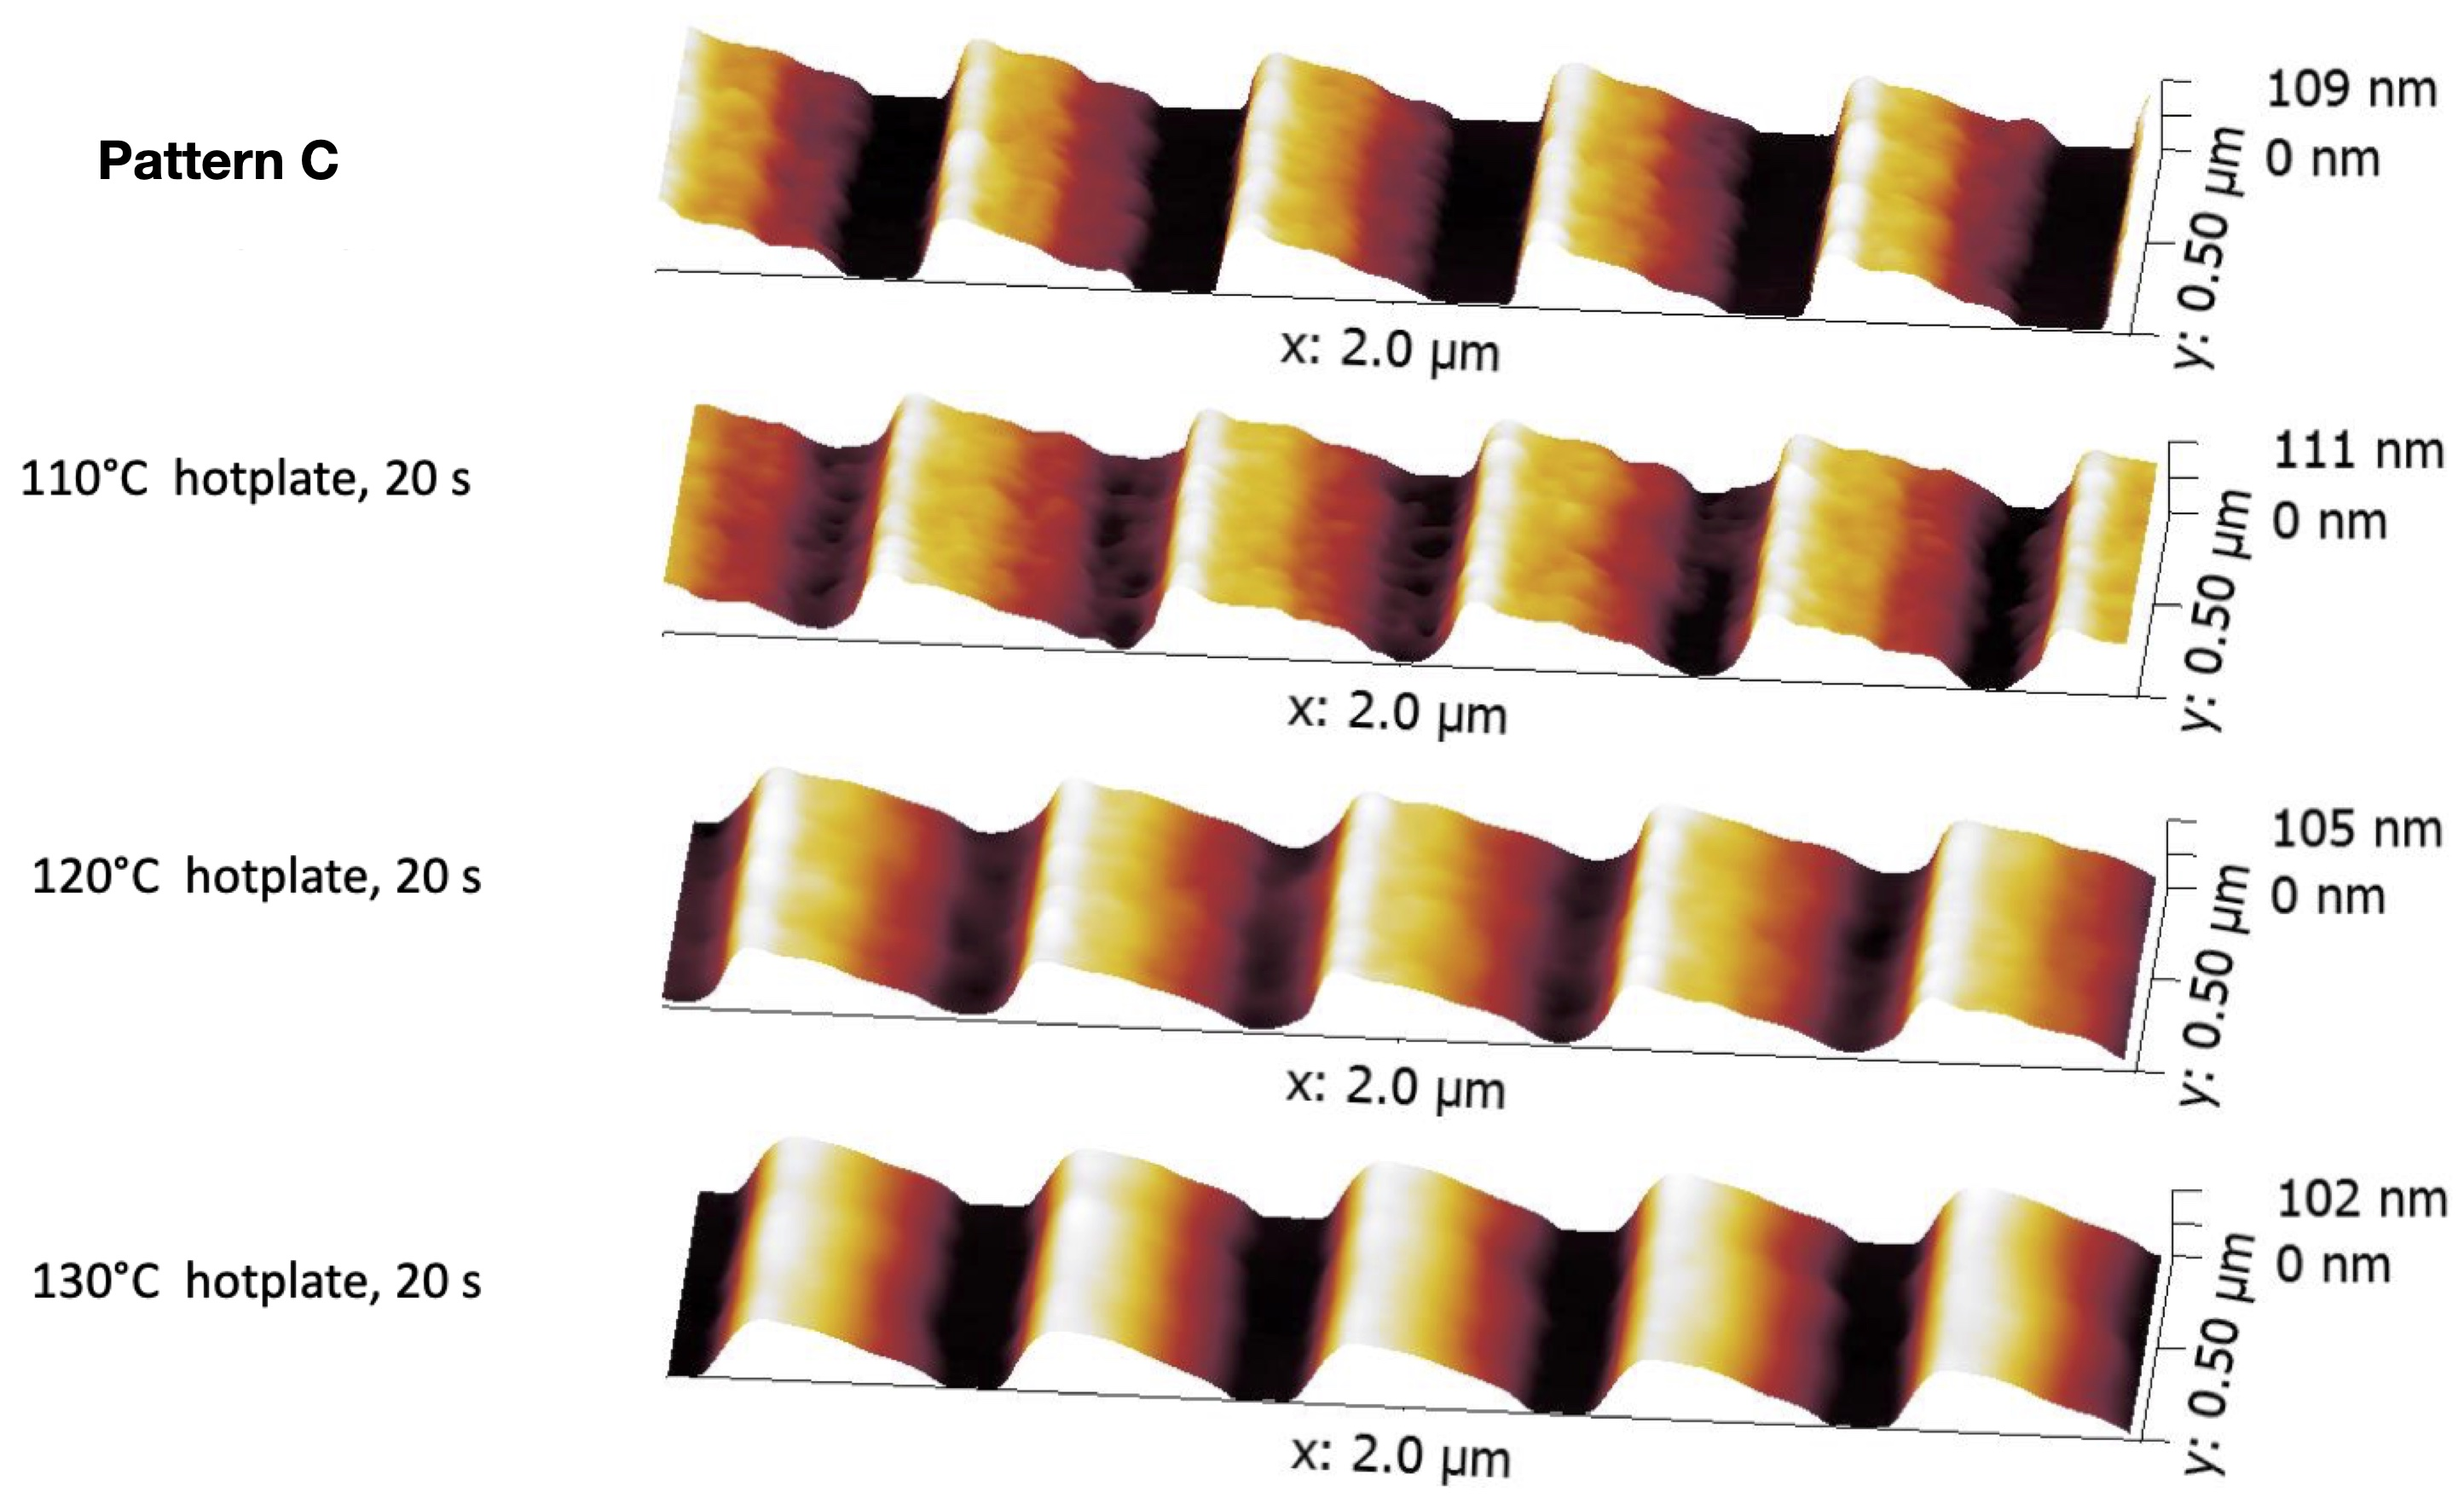
\includegraphics[scale=0.1505]{Chapter-3/Figures/C_temp_scan.jpg}
 \caption[Thermal reflow results as a function of heating temperature for grayscale pattern C]{Thermal reflow results as a function of $T$ for GEBL in \SI{130}{\nm}-thick PMMA with \num{4} levels: the width of the top level is reduced to \SI{40}{\nm} while remaining levels are \SI{120}{\nm} wide to give $d = \SI{400}{\nm}$ \cite{McCoy18}.}\label{fig:C_temp_scan}
 \end{figure}
\begin{figure}
 \centering
 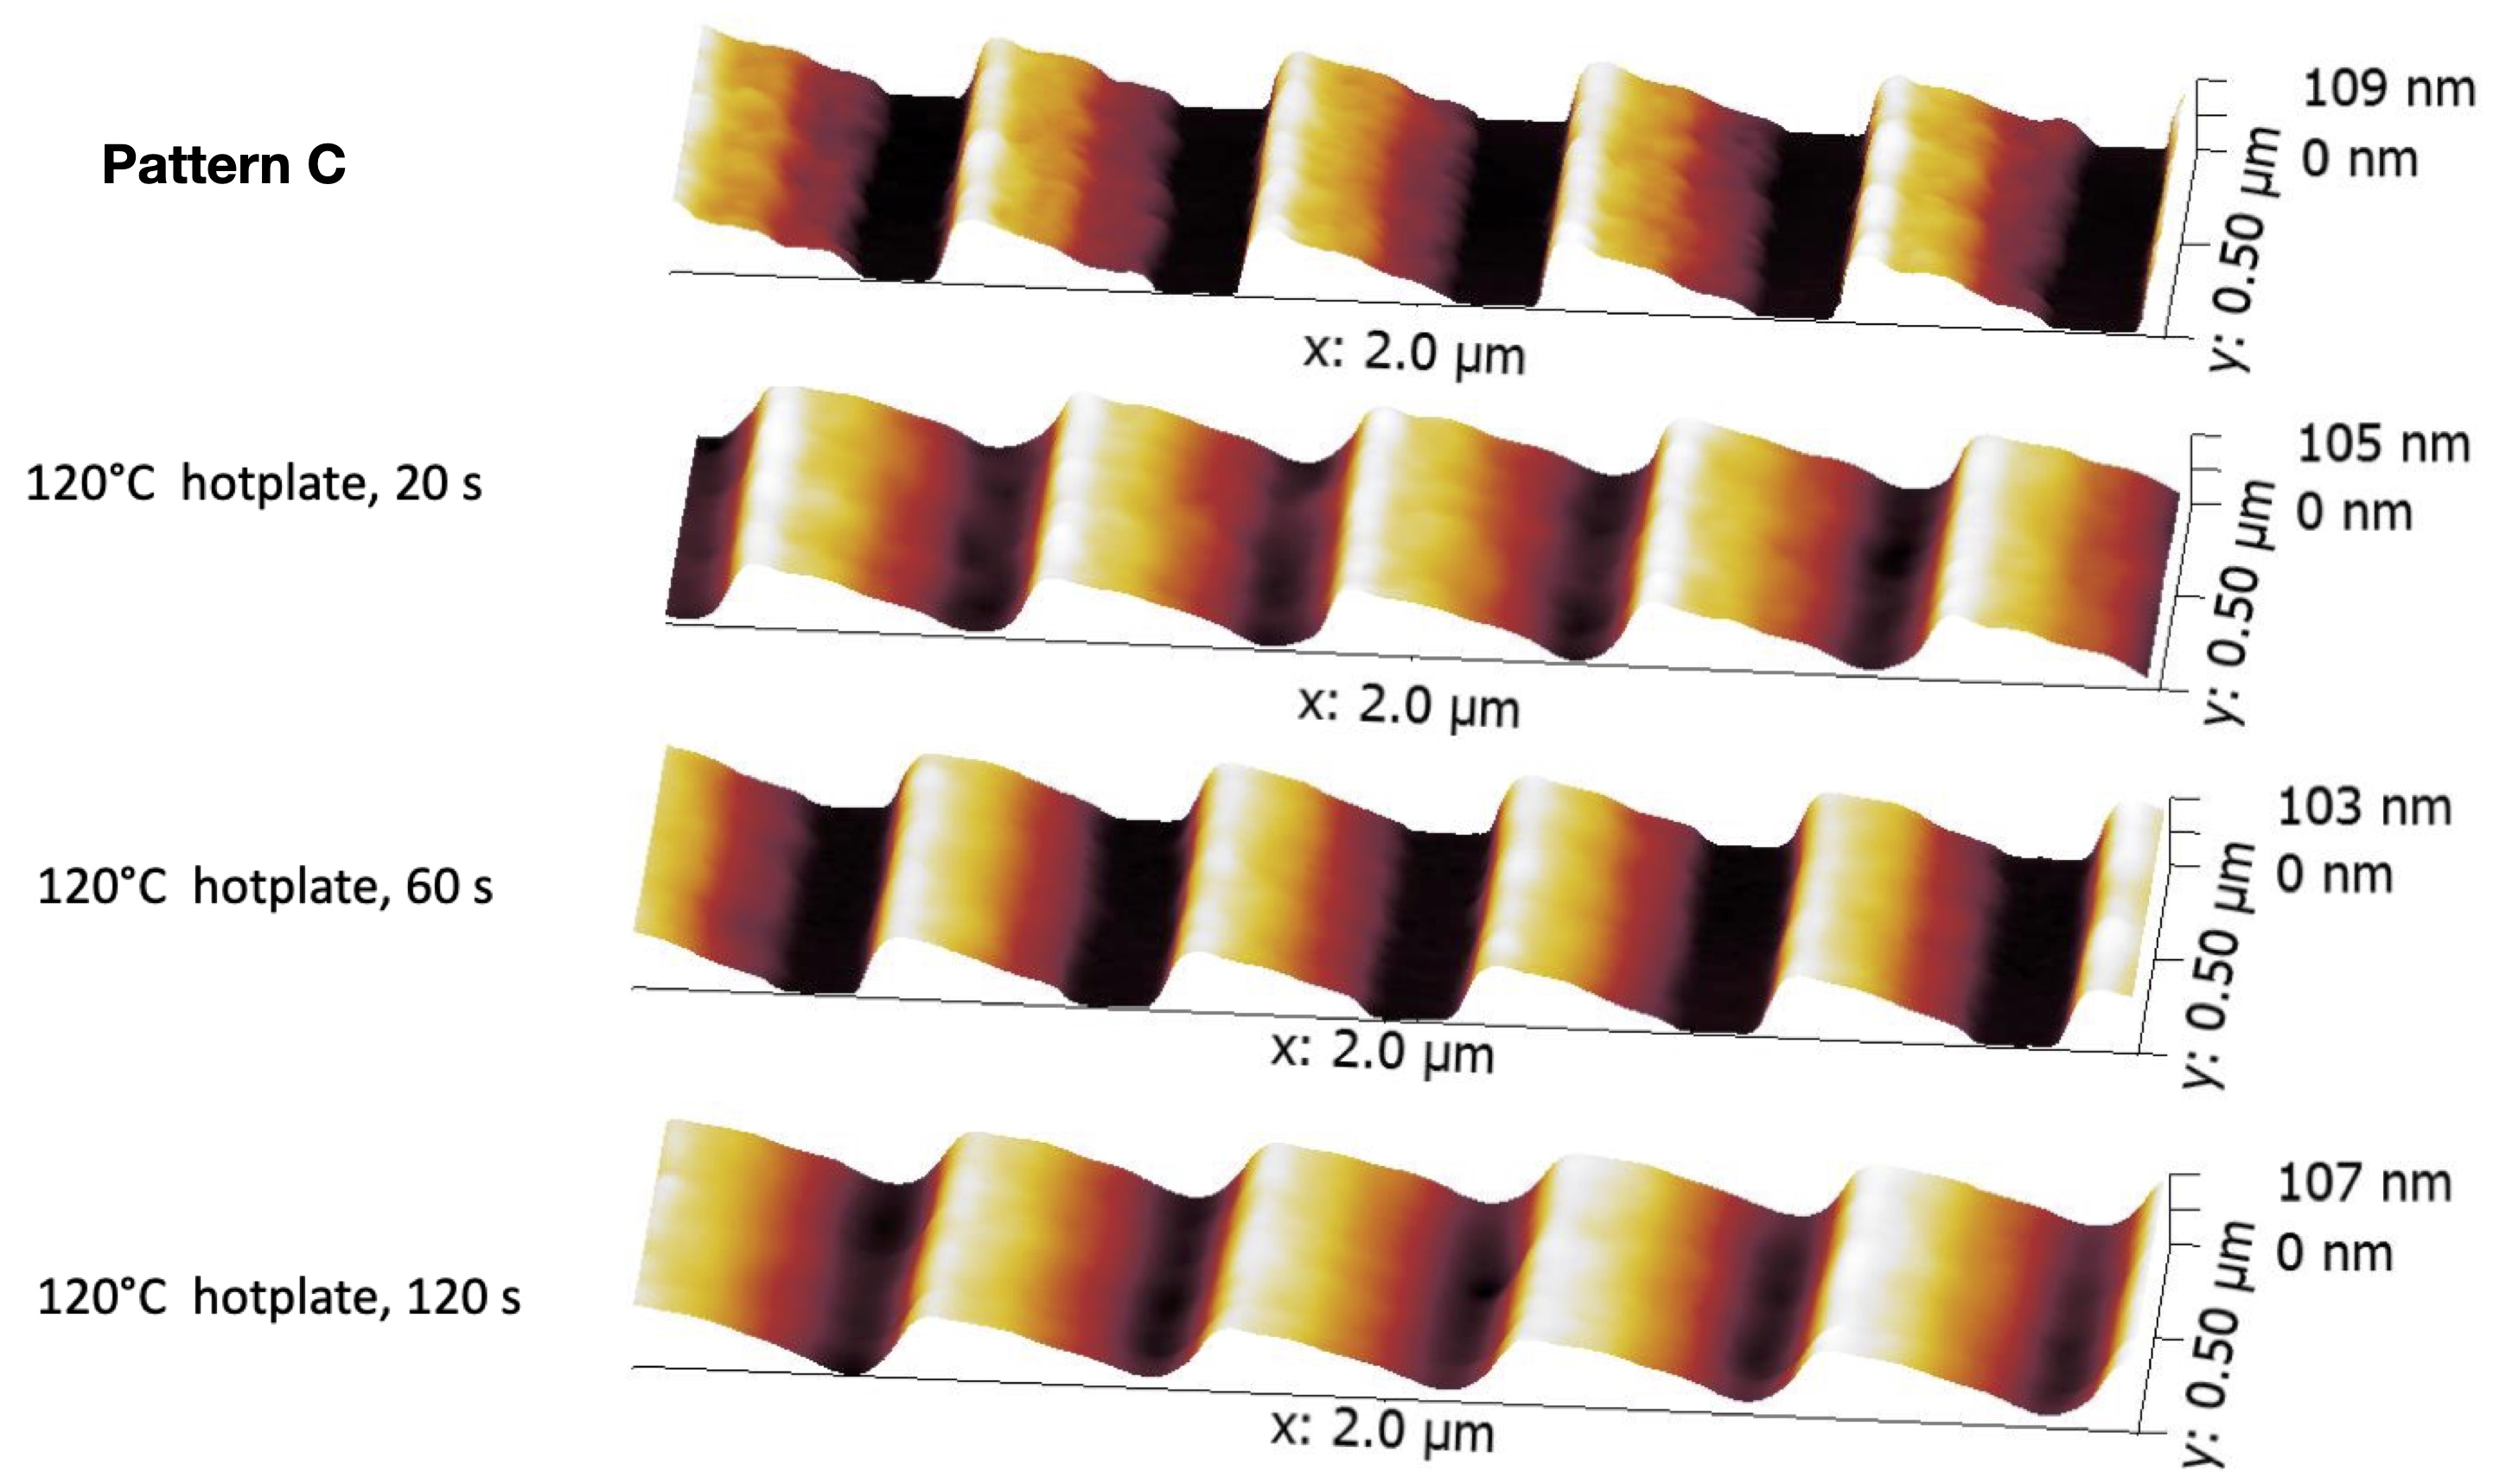
\includegraphics[scale=0.1505]{Chapter-3/Figures/C_time_scan.jpg}
 \caption[Thermal reflow results as a function of heating duration for grayscale pattern C]{Thermal reflow results as a function of $t$ for GEBL in \SI{130}{\nm}-thick PMMA with \num{4} levels as in \cref{fig:C_temp_scan} \cite{McCoy18}.}\label{fig:C_time_scan}
 \end{figure}
These initial results demonstrate the principle of TASTE: stepped surfaces of resist begin to smooth into inclines with an appropriate thermal treatment. 
However, only a small sample of the $T$-$t$ parameter space for TASTE has been explored. 
The reflow temperature should be optimized such that intermediate steps are able to flow while the top step is unaffected; this is to achieve a sharp sawtooth by avoiding groove rounding effects. 
Meanwhile, heating duration should also be optimized to allow flowing resist to equilibrate into smooth, sloped surfaces. 
Preferred temperature-time parameters will depend on the initial GEBL structure. 

Shown under AFM in \cref{fig:A_temp_scan}, a small reflow effect at $T = \SI{110}{\celsius}$ is seen in the intermediate steps of pattern A. 
The effect becomes more pronounced at $T = \SI{120}{\celsius}$ while at $T = \SI{130}{\celsius}$, the entire structure, including the top step, is noticeably affected. 
Holding $T = \SI{120}{\celsius}$ constant as in \cref{fig:A_time_scan}, the intermediate steps become increasingly smooth with increasing $t$. 
At $t = \SI{120}{\second}$, however, it appears that equilibration has not yet been reached as evidenced by the slight waviness on the facets left over from the GEBL staircase steps. 
This suggests that the optimum temperature for TASTE of pattern A is close to $T_{\text{reflow}} = \SI{120}{\celsius}$ while the reflow duration required for equilibration is $t > \SI{120}{\second}$. 
Shown in \cref{fig:B_temp_scan,fig:B_time_scan,fig:C_temp_scan,fig:C_time_scan}, a similar effect is observed for patterns B and C. 
However, the optimum reflow temperature for patterns B and C may be slightly lower as the narrowed top step in each case is expected to have a reduced $M_w$ relative to that of pattern A. 
This is evidenced by the $\sim \SI{25}{\percent}$ reduction in structure height relative to the original film thickness, as mentioned previously, and the slight rounding observed in the top step at $T = \SI{120}{\celsius}$ for $t = \SI{120}{\second}$, which both reflect a slightly lowered $T_{\text{reflow}}$ as compared to pattern A. 
In these cases, selectivity for equilibration is degraded such that the top step experiences a small degree of viscous flow along with other steps, and as a result, the overall structure exhibits a convex-like quality at the groove apex along with a quasi-linear slope that emulates a blazed facet. 

\section[Grating Prototype Fabrication]{Grating Prototype Fabrication}\label{sec:TASTE_prototype} 
%%%%%%%%%%%%%%%%%%%%%%%%%%%%%%%%%%%%%%%%%-------------------------------------------------
Although not exhaustive, the TASTE results presented in \cref{sec:reflow_results} show that a process window exists to transform a repeating staircase structure fabricated by GEBL into a sawtooth-like surface relief using thermal reflow. 
The experimentation described in this section leverages from the process development outlined in \cref{sec:TASTE} to fabricate a blazed grating prototype that is suitable for soft x-ray diffraction-efficiency testing in an extreme off-plane mount. 
Based on the layout for \emph{pattern B} introduced in \cref{sec:GEBL}, this grating prototype was designed to have $d = \SI{400}{\nm}$, and from the AFM-measured angle of the sawtooth facets in $\SI{130}{\nm}$-thick PMMA [\emph{cf.\@} \cref{fig:B_temp_scan,fig:B_time_scan}], the effective blaze angle is expected to be $\delta \approx 27^{\circ}$. %a groove spacing of
In a near-Littrow configuration for an extreme off-plane geometry with order locations given by the generalized grating equation \cite[\emph{cf.\@} \cref{eq:off-plane_orders,eq:off-plane_orders_ch2,eq:off-plane_incidence_orders}]{Loewen97}, the azimuthal incidence angle [\emph{cf.\@} \cref{fig:conical_reflection_edit,fig:grating_angles}] is $\alpha \approx \delta$ while the groove-facet incidence angle is $\zeta \lessapprox \gamma$ by \cref{eq:angle_on_groove}, where $\gamma$ is the cone opening half-angle of the diffraction pattern. 
This grazing-incidence angle $\gamma$ must be smaller than the critical angle for \emph{total external reflection (TER)} of the grating material, $\zeta_c (\omega)$ [\emph{cf.\@} \cref{sec:als_testing}]. 
To satisfy these conditions, the grating prototype was designed for use at a nominal graze angle of $\eta = 1.5^{\circ}$ in a Littrow configuration, where $\alpha = \beta = \delta \approx 27^{\circ}$ and $\zeta = \gamma \approx 1.7^{\circ}$ by \cref{eq:angle_on_groove,eq:graze_angle} with \cref{eq:blaze_wavelength} for the blaze wavelength becoming  
\begin{equation}\label{eq:blaze_wavelength_TASTE}
 \lambda_b = \frac{2 d \sin \left( \gamma \right) \sin \left( \delta \right) }{n} \approx \frac{\SI{11}{\nm}}{n} ,
 \end{equation}
which provides an estimate for the spectral locations of peak orders [\emph{cf.\@} \cref{fig:pcgrate_example_au}]. 

As described in \cref{sec:als_testing}, a grating geometry defined by $\alpha$ and $\gamma$ is parameterized by the principal-axis angles $\eta$, $\varphi$ and $\phi$ at beamline 6.3.2 of the ALS [\emph{cf.\@} \cref{fig:grating_angles,fig:ALS_arc}]. 
With $\eta = 1.5^{\circ}$, \cref{eq:yaw_angle} yields $\varphi \approx 0.8^{\circ}$ so that for $\phi \approx 0^{\circ}$, the grating-dispersion direction is virtually parallel to the direction of the horizontal linear stage motion [\emph{cf.\@} \cref{sec:geo_constrain}]. 
Because the incident beam is then nearly parallel with both the groove direction and the surface of the grating substrate, the grooves of the grating prototype must be long enough to encompass the incident beam in projection at the chosen value of $\eta \approx 1.5^{\circ}$. 
With knowledge that the cross-sectional size of the beam at the ALS is $\lessapprox \SI{0.5}{\mm}$ as it is incident on an optic, the grating prototype was designed to be \SI{50}{\mm} along the groove direction and \SI{7.5}{\mm} along the grating-dispersion direction so as to allow the beam to be positioned on the grooved area with relative ease. 
Considering the wavelengths of radiation at which there exist propagating orders in this geometry and the separation of these orders defined by \cref{eq:linear_dispersion} with $d = \SI{400}{\nm}$ and $L \approx \SI{235}{\mm}$ relative to the \SI{0.5}{\mm} slit width, diffraction-efficiency testing was carried out over $\SI{15.5}{\nm} \gtrapprox \lambda \gtrapprox \SI{1.55}{\nm}$, or equivalently, extreme ultraviolet (EUV) and soft x-ray photon energies, $\mathcal{E}_{\gamma}$, ranging from \SIrange{80}{800}{\electronvolt}. 

\subsection{TASTE Processing}\label{sec:prototype_TASTE_process}
%%%%%%%%%%%%%%%%%%%%%%%%%%%%%%%%%%%%%%%%%--------------------------------------------------
GEBL processing for fabrication of the grating-prototype surface relief is outlined in \cref{fig:TASTE_diagram}: the staircase topography features two electron-exposed steps, a cleared area and an unexposed step, all of equal width consistent with a periodicity of $d = \SI{400}{\nm}$.\footnote{\emph{i.e.}, $w_0 = w_1 = w_2 = w_3 = \SI{100}{\nm}$} 
Electron dosing for GEBL was performed according to the resist-contrast curve provided in \cref{sec:resist_contrast}, which is based on a room-temperature development recipe consisting of \SI{2}{\minute} in 1:1 MIBK/IPA followed by a \SI{30}{\second} rinse in IPA and a high-purity nitrogen blow-dry. 
This contrast curve is shown in \cref{fig:resist_contrast}, where post-development PMMA thickness as measured by SE is plotted as a function of assigned electron dose, $D$. 
These data were processed using the \textsc{Layout BEAMER 3DPEC} algorithm [\emph{cf.\@} \cref{sec:GEBL}] to generate a dose-corrected layout appropriate for achieving exposed staircase steps with $h_1 \approx 0.66 h_0$ and $h_2 \approx 0.33 h_0$, where $h_0 \approx \SI{130}{\nm}$ is the spin-coat thickness. 
Electron exposure for GEBL was carried out using an \SI{8}{\nano\ampere} beam current and a \SI{400}{\um} aperture with a beam step size and a writing-grid resolution of \SI{10}{\nm}, which is comparable to the beam spot size realized by the \textsc{EBPG5200} under these conditions. 
Due to a \SI{100}{\mega\hertz} clock frequency upgrade to the \textsc{EBPG5200} at Penn State in 2018, these beam conditions differ from the recipe described in \cref{sec:GEBL}, which was limited by the \SI{25}{\mega\hertz} frequency at the time of the experiment \cite{McCoy18,McCoy20}. %

Using the GEBL process outlined above, test patterns were exposed, wet-developed and characterized by AFM to verify that the previously-reported staircase topography could be readily reproduced using the increased value for beam current enabled by a \SI{100}{\mega\hertz} clock frequency. 
\begin{figure}
 \centering
 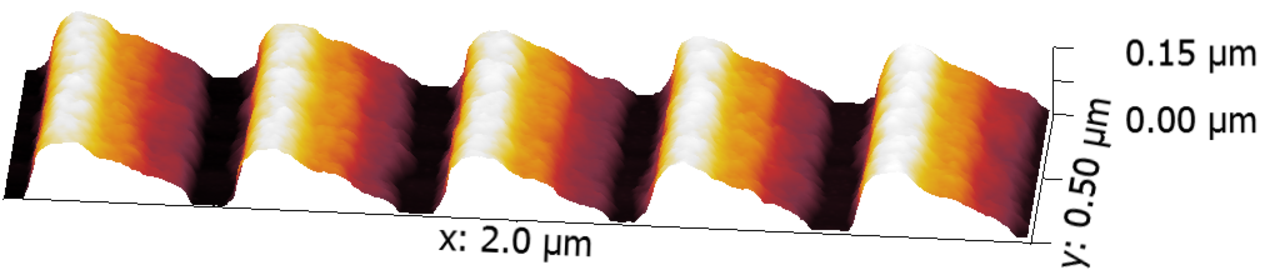
\includegraphics[scale=0.7]{Chapter-3/Figures/grayscale_AFM.pdf}
 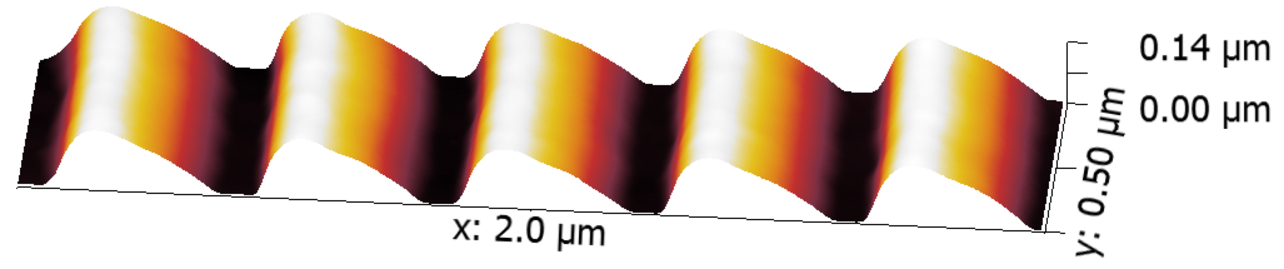
\includegraphics[scale=0.7]{Chapter-3/Figures/reflow_AFM.pdf}
 \caption[AFMs of the GEBL-processed resist and the resist following thermal reflow.]{AFMs of the GEBL-processed resist (\emph{top}) and the resist following thermal reflow (\emph{bottom}) \cite{McCoy20}.}\label{fig:TASTE_AFMs}
 \end{figure}
As in \cref{sec:TASTE}, AFM was carried out over \SI{2}{\um} in the grating-dispersion direction at \num{512} samples per line to yield a \SI{3.9}{\nm} pixel size.  
A scan of the GEBL pattern exposed using an \SI{8}{\nano\ampere} beam current and a \SI{400}{\um} aperture is shown in the top panel of \cref{fig:TASTE_AFMs}, where it is verified that the topography appears virtually indistinguishable from the previous result from \cref{sec:TASTE} obtained using a \SI{1}{\nano\ampere} beam current and a \SI{200}{\um} aperture. 
Next, thermal-reflow experimentation on test samples was carried out using an automated hotplate tool built by \textsc{Fusion Semiconductor} [\emph{cf.\@} \cref{sec:reflow_results}], where from the results reported in \cref{sec:TASTE}, it is expected that the optimum value for $T_{\text{reflow}}$ is near \SI{120}{\celsius}. 
Through a series of reflow tests, it was found that $T_{\text{reflow}} = \SI{116}{\celsius}$ applied for a duration of \SI{30}{\minute}\footnote{Due to the \SI{999}{\second} time-out of the \textsc{Fusion Semiconductor} automated hotplate tool, thermal reflow was carried out in two consecutive \SI{15}{\minute} intervals.} produced a topography that most closely resembled a sawtooth. 
An AFM of a test pattern hotplate-treated in this way is shown in the bottom panel of \cref{fig:TASTE_AFMs}, where a slight convex quality is observed, which is likely a result of degraded reflow selectivity [\emph{cf.\@} \cref{sec:TASTE_ch5}]. % as discussed further in \cref{sec:TASTE_ch5}.  
Nonetheless, the overall structure resembles a sawtooth and based on these results, a \SI{7.5}{\mm} by \SI{50}{\mm} area was exposed for GEBL using a \SI{300}{\um} by \SI{300}{\um} mainfield with \SI{10}{\nm} resolution, a \SI{4}{\um} by \SI{4}{\um} subfield with \SI{5}{\nm} resolution and \textsc{Large Rectangle Fine Trapezoid} fracturing in \textsc{Layout Beamer} \cite{beamer}. 
\begin{figure}
 \centering
 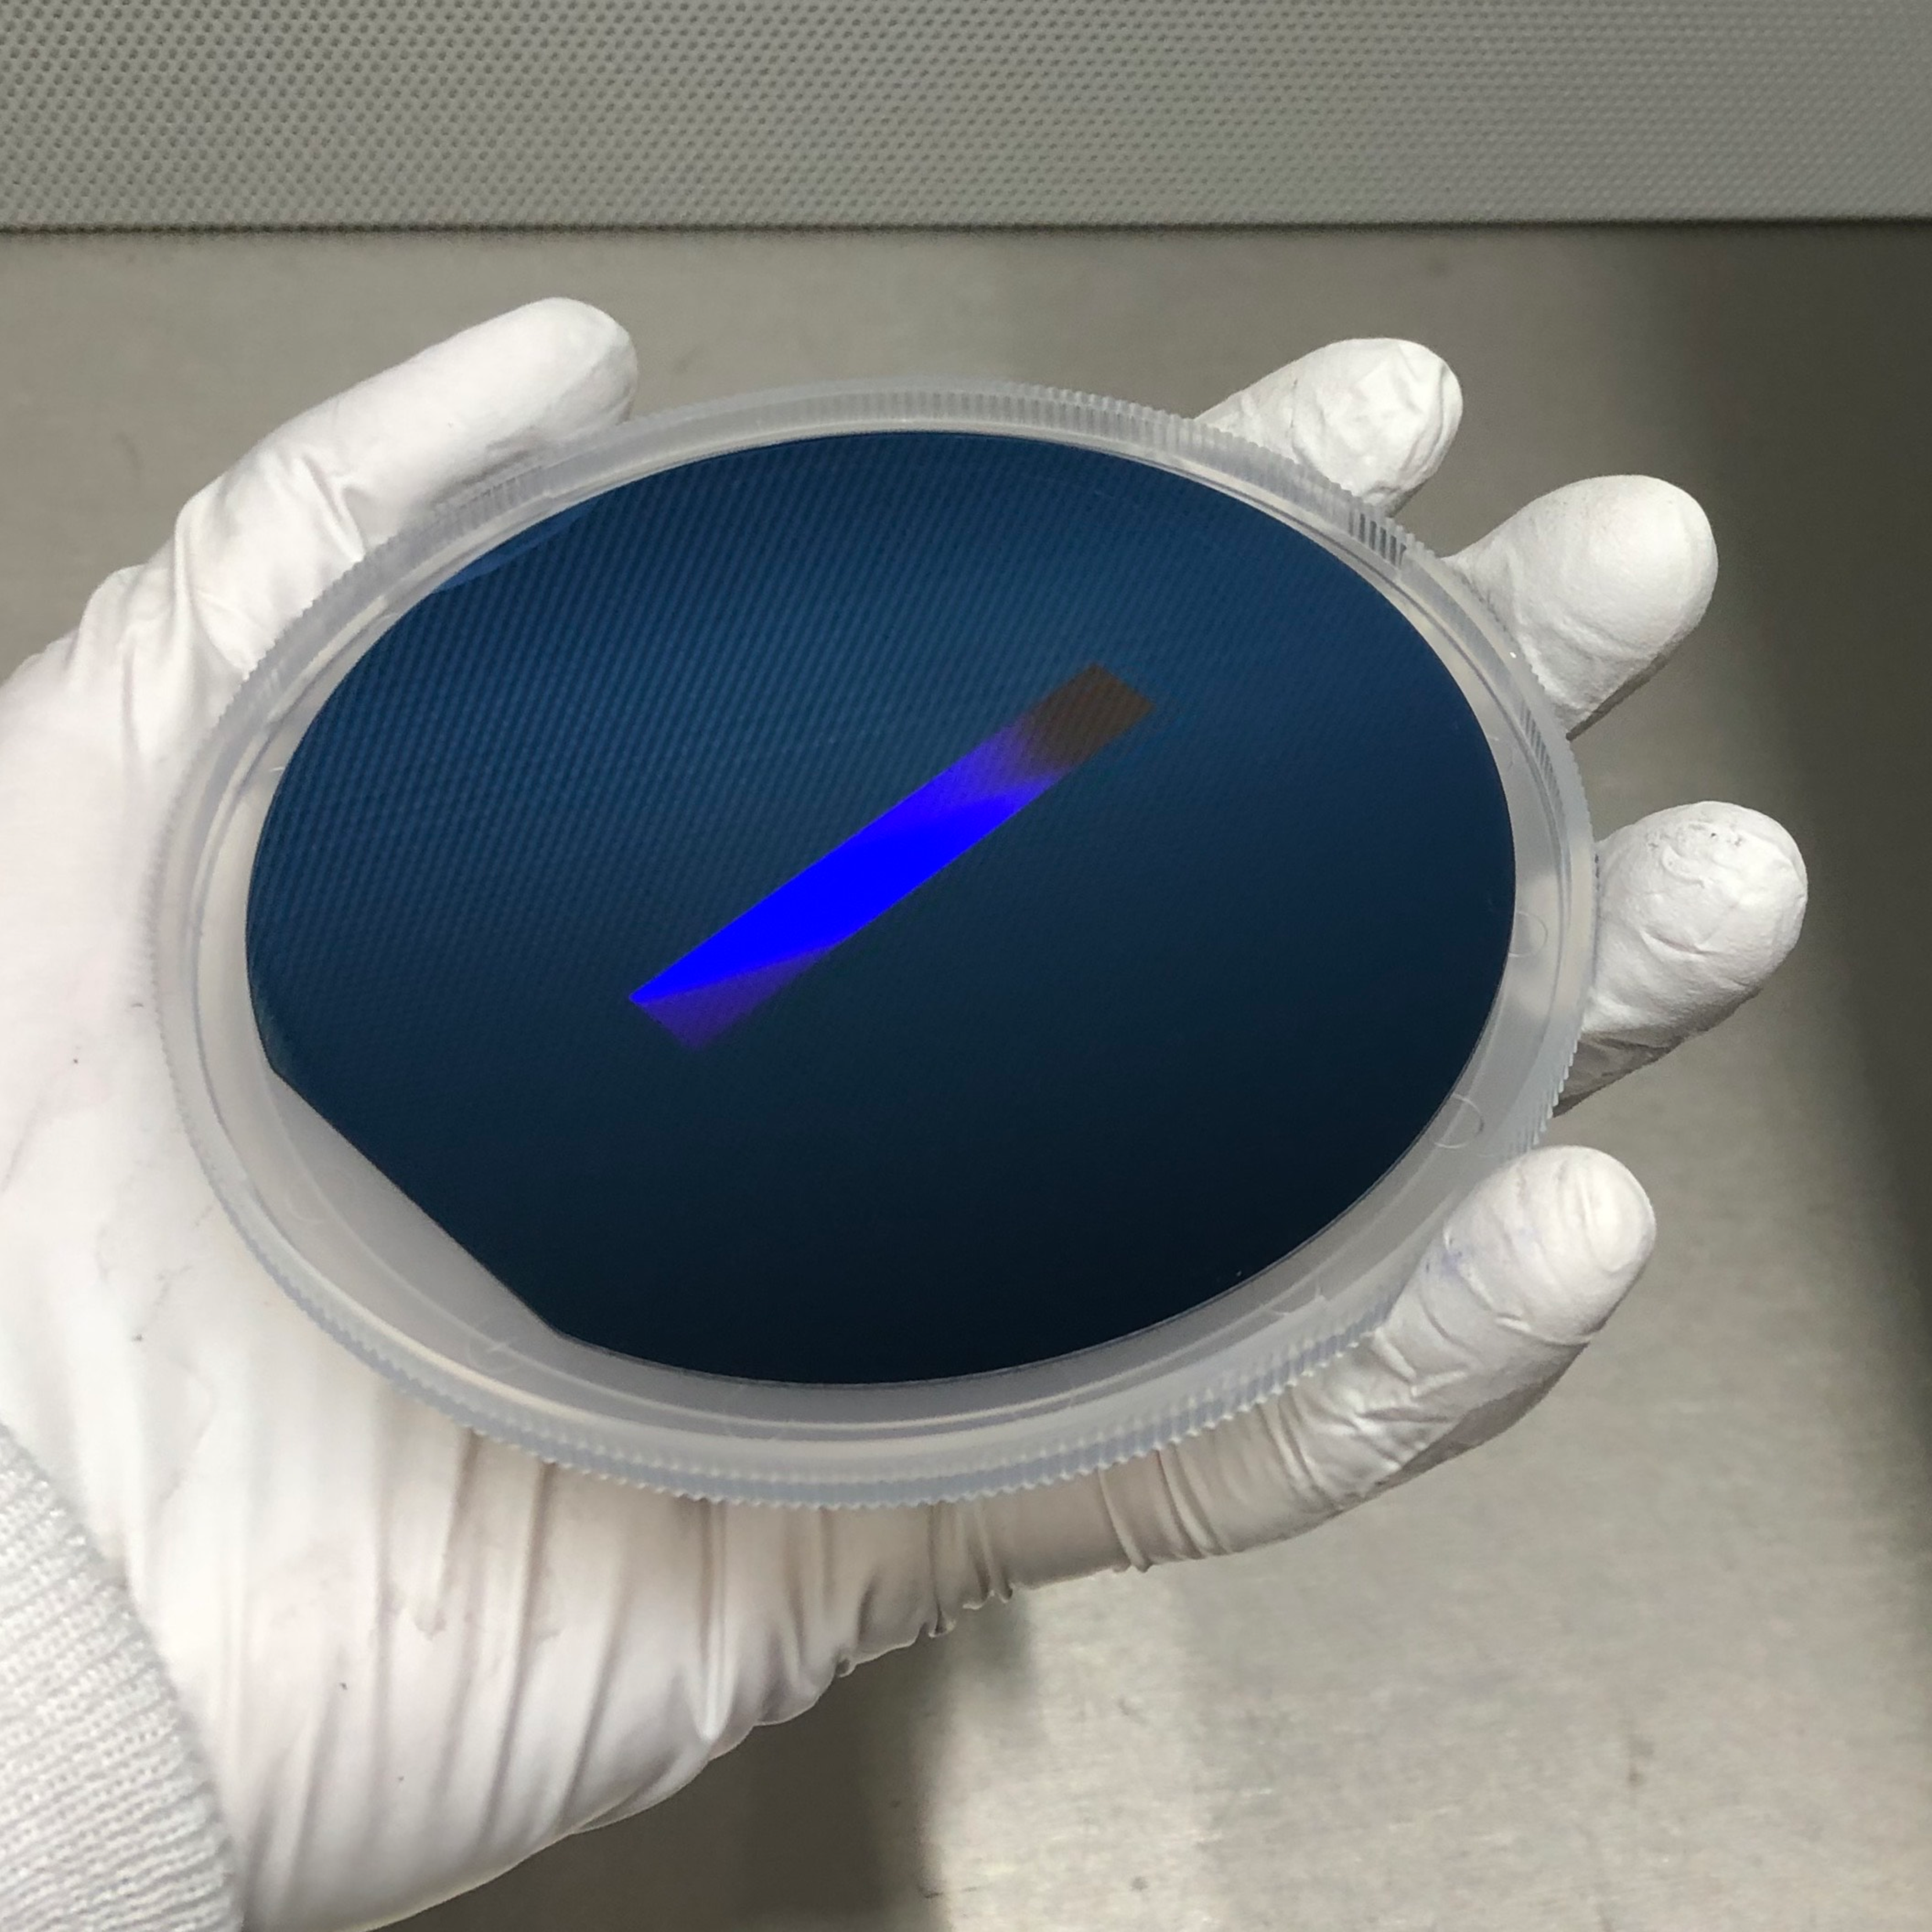
\includegraphics[scale=0.15]{Chapter-3/Figures/uncoated_grating_photo.pdf}
 \caption[Photograph of the (uncoated) grating prototype patterned in \SI{130}{\nm}-thick PMMA on a \SI{100}{\mm}-diameter silicon wafer using TASTE.]{Surface-relief mold for the grating prototype patterned in \SI{130}{\nm}-thick PMMA on a \SI{100}{\mm}-diameter silicon wafer using TASTE. The grating measures \SI{50}{\mm} in the groove direction and \SI{7.5}{\mm} in the grating-dispersion direction \cite{McCoy20}.}\label{fig:uncoated_grating_pic}
 \end{figure}
Under these conditions, the \textsc{EBPG5200} exposure duration (including tool overhead) was $\lessapprox \SI{20}{\hour}$. 
The grating mold resulting from the entire TASTE process patterned on a \SI{100}{\mm}-diameter wafer is pictured in \cref{fig:uncoated_grating_pic}. 

\subsection{Coating for Reflectivity}\label{sec:prototype_coating}
%%%%%%%%%%%%%%%%%%%%%%%%%%%%%%%%%%%%%%%%%--------------------------------------------------
Although achieving an effective blaze response from the grating prototype hinges on the shape of the sawtooth facets produced by TASTE, \emph{absolute diffraction efficiency}, $\mathscr{E}_n$, is also dependent on the reflectivity of the sawtooth facets at a nominal incidence angle $\zeta \approx 1.7^{\circ}$ [\emph{cf.\@} \cref{ch:diff_eff}]. 
Having an overcoating on the grating surface relief described in \cref{sec:prototype_TASTE_process} is important primarily for avoiding prominent absorption edges of carbon and oxygen in PMMA and for achieving high overall reflectivity at this value of $\zeta$ [\emph{cf.\@} \cref{fig:X-ray_index,fig:X-ray_refl}]. 
As described in \cref{sec:reflectivity_polarization}, Fresnel reflectivity, $\mathcal{R}_F$, is virtually insensitive to polarization and hence the quantity can be expressed in s-polarization with a high degree of accuracy.  
For a thick slab of material realized by a film thickness several times larger than the $1 / \mathrm{e}$ \emph{penetration depth} for radiation under TER [\emph{cf.\@} \cref{sec:total_refl,eq:penetration_depth}]: 
\begin{equation}\label{eq:ch3_pene_dep}
 \mathcal{D}_{\perp} = \frac{\lambda}{4 \pi \, \text{Im} \! \left[ \sqrt{\tilde{\nu}^2 (\omega) - \cos^2 \left( \zeta \right)} \right]} ,
 \end{equation}
$\mathcal{R}_F$ in s-polarization is given by \cref{eq:s_reflectivity}: %[\emph{cf.\@} \cref{eq:s_reflectivity}]
\begin{equation}\label{eq:ch3_fres_refl}
 \mathcal{R}_F = \norm{ \frac{\sin \left( \zeta \right) - \sqrt{\tilde{\nu}^2 (\omega) - \cos^2 \left( \zeta \right)}}{\sin \left( \zeta \right) + \sqrt{\tilde{\nu}^2 (\omega) - \cos^2 \left( \zeta \right)}} }^2 , 
 \end{equation}
where $\tilde{\nu} (\omega) = 1 - \delta_{\nu} (\omega) + i \xi (\omega)$ is the complex index of the material tabulated by the CXRO online database \cite[\emph{cf.\@} \cref{tab:optical_constants}]{CXRO_database}. 
\begin{figure}
 \centering
 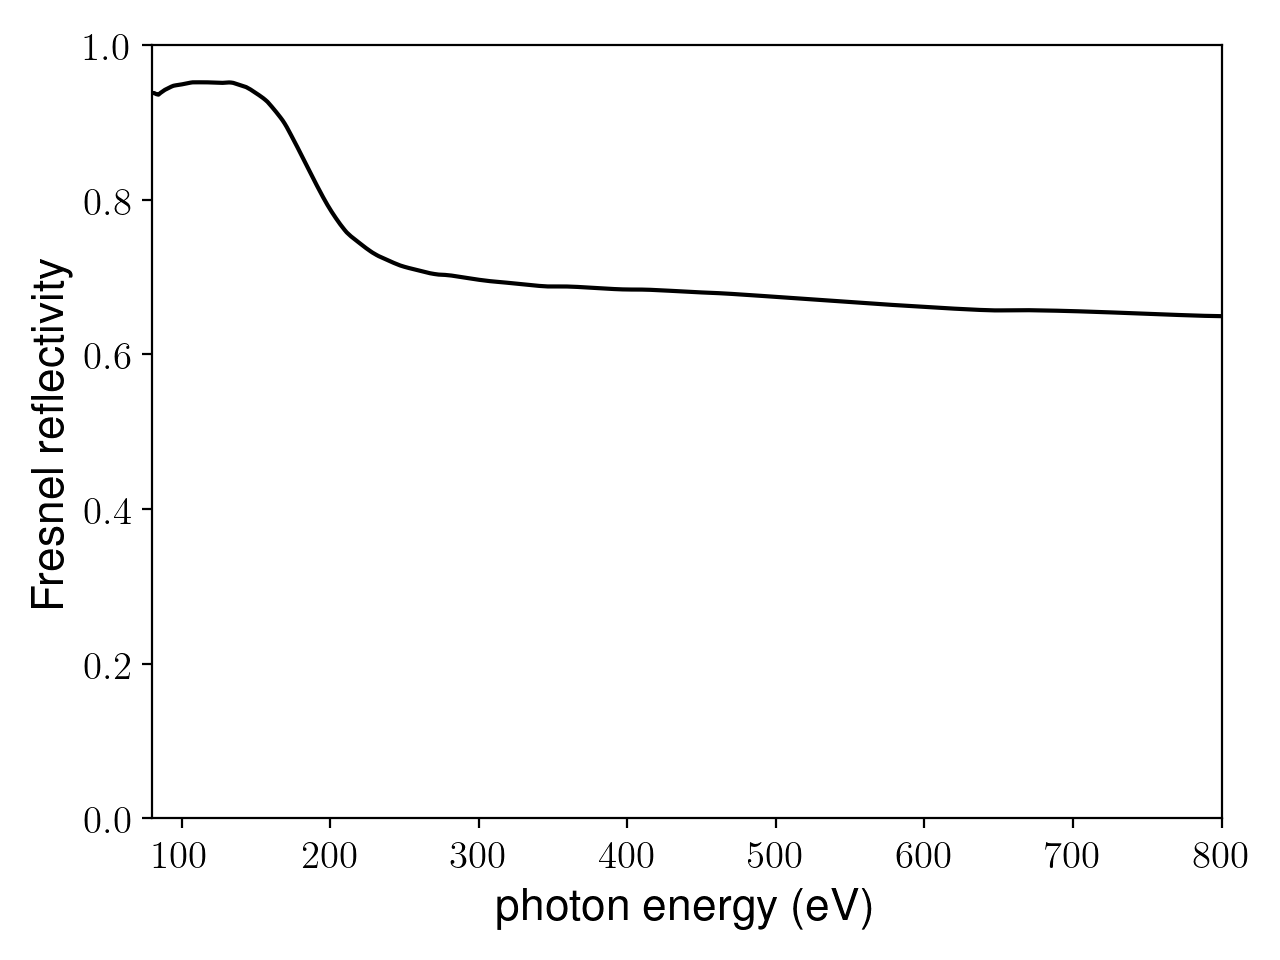
\includegraphics[scale=0.75]{Chapter-3/Figures/reflectivity.png}
 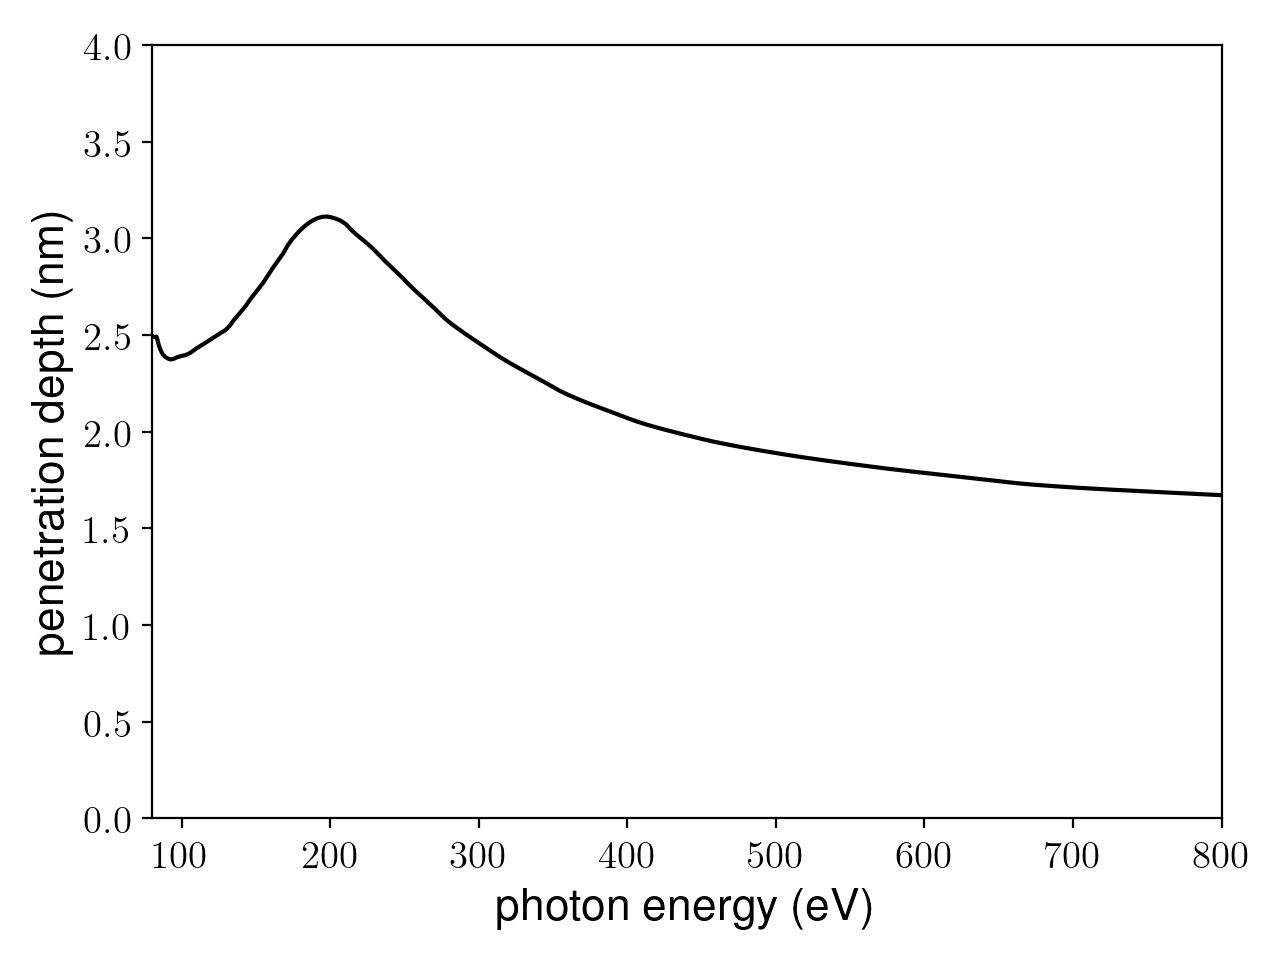
\includegraphics[scale=0.75]{Chapter-3/Figures/attn_depth.png}
 \caption[Fresnel reflectivity and penetration depth in a thick slab of gold for nominal test geometry]{Fresnel reflectivity, $\mathcal{R}_F$, and penetration depth, $\mathcal{D}_{\perp}$, in a thick slab of gold at $\zeta = 1.7^{\circ}$ over $\SI{80}{\electronvolt} \leq  \mathcal{E}_{\gamma} \leq \SI{800}{\electronvolt}$ (data obtained from CXRO \cite{CXRO_database}) \cite{McCoy20}.}\label{fig:Au_refl_attn} %($\mathcal{R}_F$ given by \cref{eq:ch3_fres_refl}) %($\mathcal{D}_{\perp}$ given by \cref{eq:ch3_pene_dep}) 
 \end{figure}
Based on the x-ray properties of various materials examined in \cref{app:x-ray_materials}, gold is a suitable choice for this overcoat due to its high $\mathcal{R}_F$ and nanoscale $\mathcal{D}_{\perp}$ across the spectral bandpass considered [\emph{cf.\@} \cref{fig:Au_refl_attn}]. 
In principle, a $\sim \SI{15}{\nm}$-thick layer is sufficient to treat the material as a thick slab so that further reflections at underlaying material interfaces can be neglected. 

Due to its broadband response over the wavelength range for diffraction-efficiency testing, $\SI{15.5}{\nm} \gtrapprox \lambda \gtrapprox \SI{1.55}{\nm}$, gold was chosen as the reflective overcoat for the grating. 
However, because gold is non-reactive toward PMMA, a thin film of an oxidizing metal such as chromium or titanium must be first deposited on the patterned resist to promote wetting and adhesion for the top, reflective layer \cite[\emph{cf.\@} \cref{sec:reflectivity_polarization}]{Trolier-McKinstry17}. 
Ideally, the result is a gold coating that maintains the fidelity of the sawtooth topography while also realizing blazed groove facets with RMS surface roughness, $\sigma$, low enough to reduce absorption and non-specular scatter at the short $\lambda$ considered [\emph{cf.\@} \cref{sec:rough_surface}]. 
From the \emph{Fraunhofer criterion} for a smooth surface [\emph{cf.\@} \cref{eq:roughness_inequality_general}]: 
\begin{equation}\label{eq:roughness_inequality}
 \sigma < \frac{\lambda}{32 \sin \left( \zeta \right)} , 
 \end{equation}
$\sigma$ should be on the level of \SI{1}{\nm} RMS to satisfy this condition for $\SI{15.5}{\nm} \gtrapprox \lambda \gtrapprox \SI{1.55}{\nm}$. 
The impact of surface roughness, however, also depends on the the typical lateral size scale of the surface features [\emph{cf.\@} \cref{sec:discussion_taste}]. 

Deposition for the grating overcoating was performed by \emph{electron-beam physical vapor deposition (EBPVD)} \cite{Singh05} using a \textsc{Kurt J.\ Lesker Lab-18} system at the Penn State Nanofabrication Laboratory \cite{PSU_MRI_nanofab}. 
First, a \SI{5}{\nm}-thick film of titanium was deposited on the patterned TASTE wafer described in \cref{sec:prototype_TASTE_process} at a previously-determined rate of \SI{0.5}{\angstrom\per\second} under high vacuum. 
This allowed a thin oxide layer to form between the resist surface and the titanium coating, providing a wetted, metallic surface for the gold layer to adhere to. %titanium and some of the oxygen present in PMMA to form 
Without breaking vacuum, the gold was then deposited at a rate of \SI{1.0}{\angstrom\per\second} to achieve a layer $\sim \SI{15}{\nm}$ thick. 
\begin{figure}
 \centering
 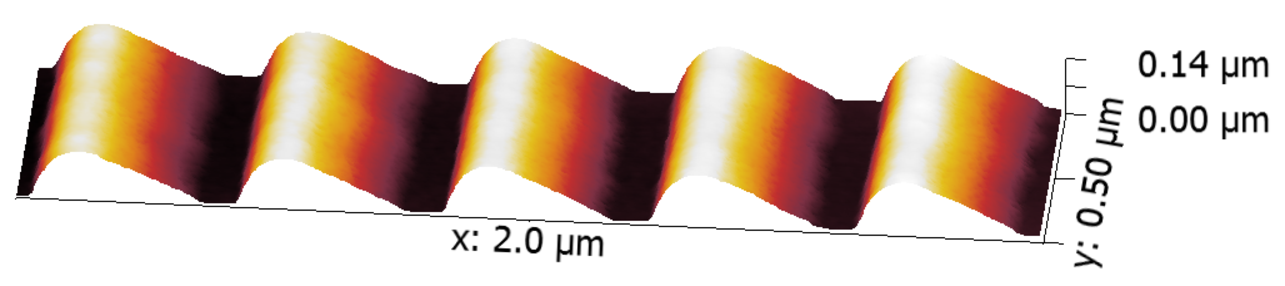
\includegraphics[scale=0.7]{Chapter-3/Figures/coating_AFM.pdf}
 \caption[AFM of the grating prototype grooves following electron-beam physical vapor deposition of gold, using titanium as an adhesion layer on PMMA]{AFM of the grating prototype grooves following EBPVD of gold, using titanium as an adhesion layer on PMMA \cite{McCoy20}.}\label{fig:coating_AFM}
 \end{figure}
The final, coated grating prototype appears under AFM as a sawtooth-like topography very similar to the uncoated, TASTE-processed resist from \cref{fig:TASTE_AFMs}; this image of the coated grating grooves, taken using the AFM methodology described in \cref{sec:prototype_TASTE_process}, is shown in \cref{fig:coating_AFM}. 

The coated grooves were imaged over a larger area by \emph{field-emission scanning electron microscopy (FESEM)} using a \textsc{Zeiss Leo 1530} system at the Penn State Nanofabrication Laboratory \cite{PSU_MRI_nanofab,Zhou07}; this micrograph, taken using a \SI{0.5}{\kilo\volt} electron accelerating voltage, is shown in \cref{fig:coating_SEM}. 
\begin{figure}
 \centering
 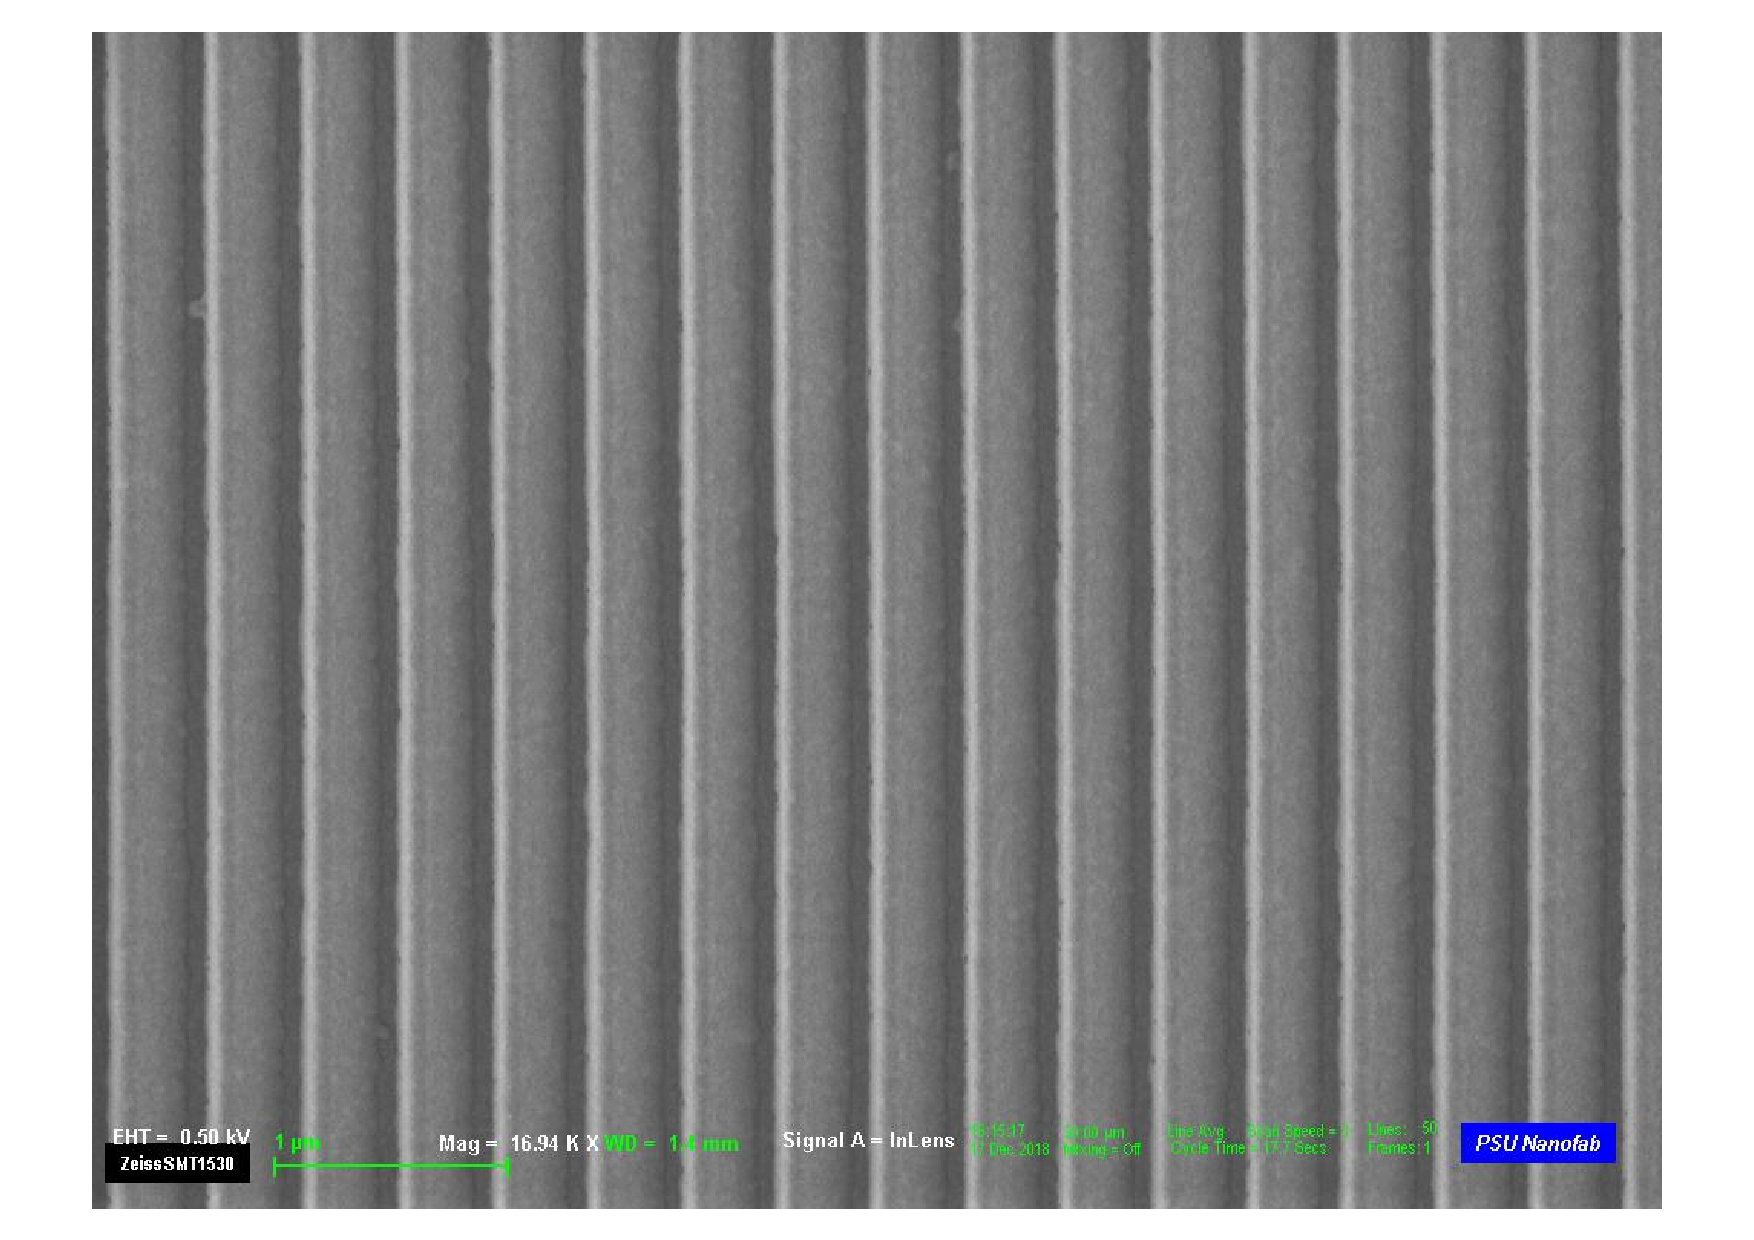
\includegraphics[scale=0.5]{Chapter-3/Figures/coated_SEM.pdf}
 \caption[FESEM of the gold-coated grating prototype grooves viewed top-down]{Field-emission scanning electron micrograph (FESEM) of the gold-coated grating prototype grooves viewed top-down, taken with a \textsc{Zeiss Leo 1530} instrument at the Penn State Nanofabrication Laboratory \cite{McCoy20}.}\label{fig:coating_SEM}
 \end{figure}
From the gathered AFM data, $\sigma$ on the groove facets measures about \SI{1.5}{\nm} RMS using the \textsc{Bruker NanoScope Analysis} software package, whereas prior to the coating [\emph{cf.\@} \cref{fig:TASTE_AFMs}, bottom panel], $\sigma \approx \SI{1.25}{\nm}$ RMS on PMMA. 
While the blaze angle measures $\delta \approx 27^{\circ}$ as expected, the groove depth measures $\sim \SI{10}{\nm}$ less than the uncoated grooves shown in \cref{fig:TASTE_AFMs}. 
Moreover, the bottom plateau of the coated grooves appears slightly widened relative to the bottom plateau of the uncoated grooves, where the surface of the silicon substrate is exposed; this suggests that the EBPVD process utilized produces a non-uniform coating, which is likely due to the geometry of the EBPVD chamber coupled with the topography of the grating grooves. 
Because these regions are to a high degree shadowed to the incoming radiation in a near-Littrow configuration, however, this is not expected to have a large impact on diffraction efficiency. 

\section{Beamline Experiments}\label{sec:taste_eff_results} 
%%%%%%%%%%%%%%%%%%%%%%%%%%%%%%%%%%%%%%%%%--------------------------------------------------
Following the methodology outlined in \cref{sec:als_testing}, the grating prototype described in \cref{sec:TASTE_prototype} was tested for EUV and soft x-ray diffraction efficiency at beamline 6.3.2 of the ALS \cite{ALS_632,Underwood96,Gullikson01}. 
The gold-coated grating prototype installed inside the beamline test chamber in an extreme off-plane mount is shown in \cref{fig:test_chamber}, where the grating-dispersion direction, $x$, is roughly parallel with the direction of horizontal stage motion for the photodiode detector, which is seen masked with a \SI{0.5}{\mm}-wide, vertical slit. 
\begin{figure}
 \centering
 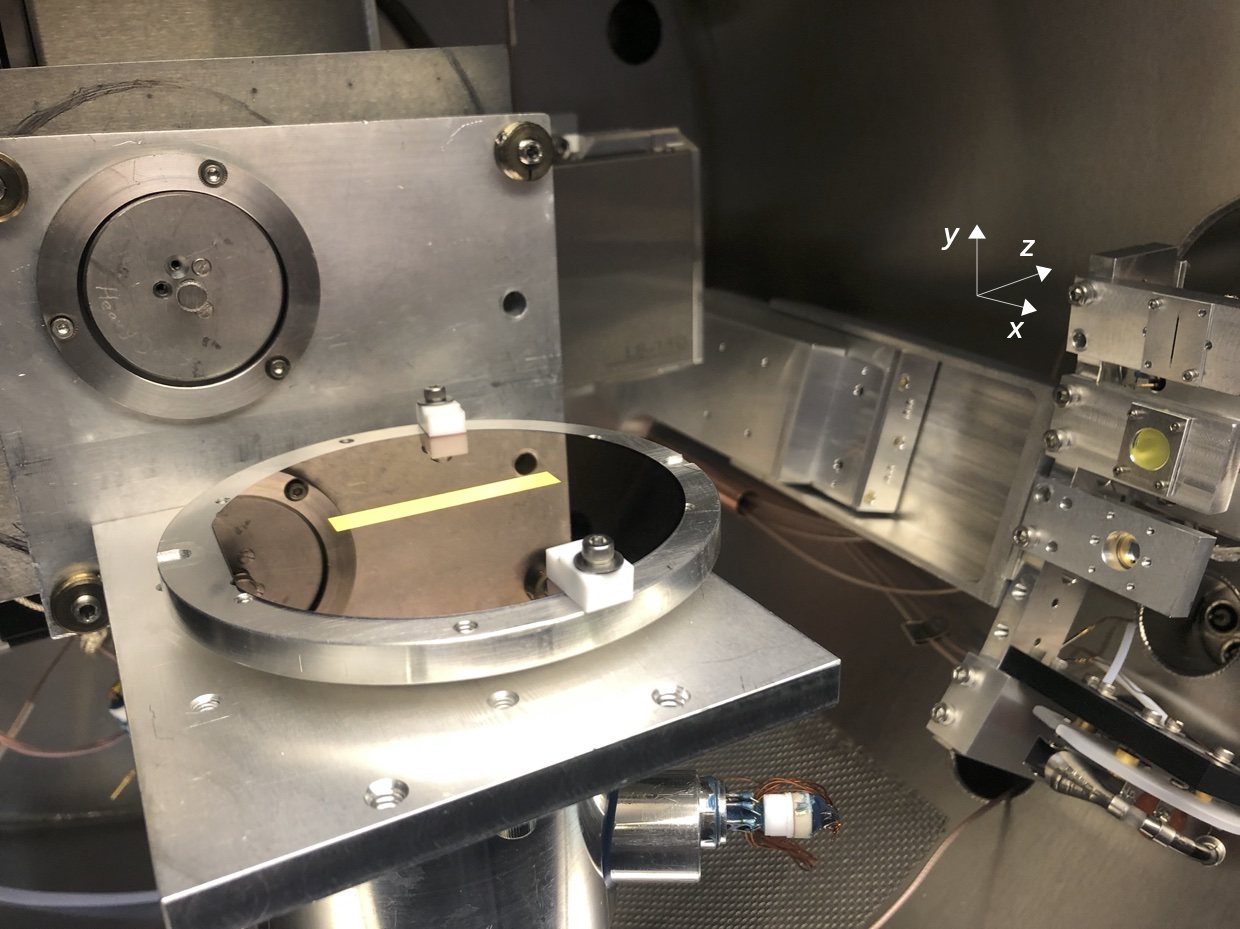
\includegraphics[scale=0.31]{Chapter-3/Figures/test_chamber_edit.jpg}
 \caption[Photograph of the TASTE grating prototype installed inside the test chamber of ALS beamline 6.3.2.]{The TASTE grating prototype [\emph{cf.\@} \cref{sec:prototype_TASTE_process,sec:prototype_coating}] installed inside the test chamber of ALS beamline 6.3.2 \cite{McCoy20}.}\label{fig:test_chamber} 
 \end{figure}
The grating was first oriented at a yaw angle of $\varphi \approx 0^{\circ}$ with graze and roll angles, $\eta$ and $\phi$ respectively, being approximately zero as measured by the tilt of the optic mount using a spirit level. 
The angle $\eta$ was then adjusted to the nominal test value of $1.5^{\circ}$ by using the goniometric stage motion of the photodiode to ensure that the angle between the direct beam and the reflected beam is roughly $2 \eta \approx 3^{\circ}$. 
Next, all grating geometric angles introduced in \cref{sec:geo_constrain} were determined experimentally through analyzing the arc of diffraction as sampled by the photodiode. 
From these measurements, the grating was set to a near-Littrow configuration by adjusting $\varphi$ to ensure that $\alpha \approx 27^{\circ}$ and $\gamma \approx 1.7^{\circ}$ at $\eta \approx 1.5^{\circ}$. 

\subsection{Constraining Grating Geometry}\label{sec:grat_geo_taste}
%%%%%%%%%%%%%%%%%%%%%%%%%%%%%%%%%%%%%%%%%--------------------------------------------------
The throw of the system at the location of $0^{\text{th}}$ order was measured to be $L = 233.0 \pm \SI{1.4}{\mm}$ by comparing the known detector length of $\ell_{\text{det}} = \SI{10}{\mm}$ to the angular size of the detector as measured by a goniometric scan of the beam [\emph{cf.\@} \cref{fig:ALS_cent_throw}]. 
Described in \cref{sec:geo_constrain}, $L$ changes as the the detector moves along the direction $x$ with focal corrections on the order of tens of \si{\um} within \SI{10}{\mm} of travel; however, these corrections are ignored so that order locations are mapped using $x$ and $y = L \sin \left( \Theta \right)$ with $L$ fixed at the measured value. 
In the final test geometry, the diffracted arc was mapped using data gathered at \SIlist{450;500}{\electronvolt} in steps of \SI{50}{\um} along the $x$-direction of the photodiode staging. 
\begin{figure}
 \centering
 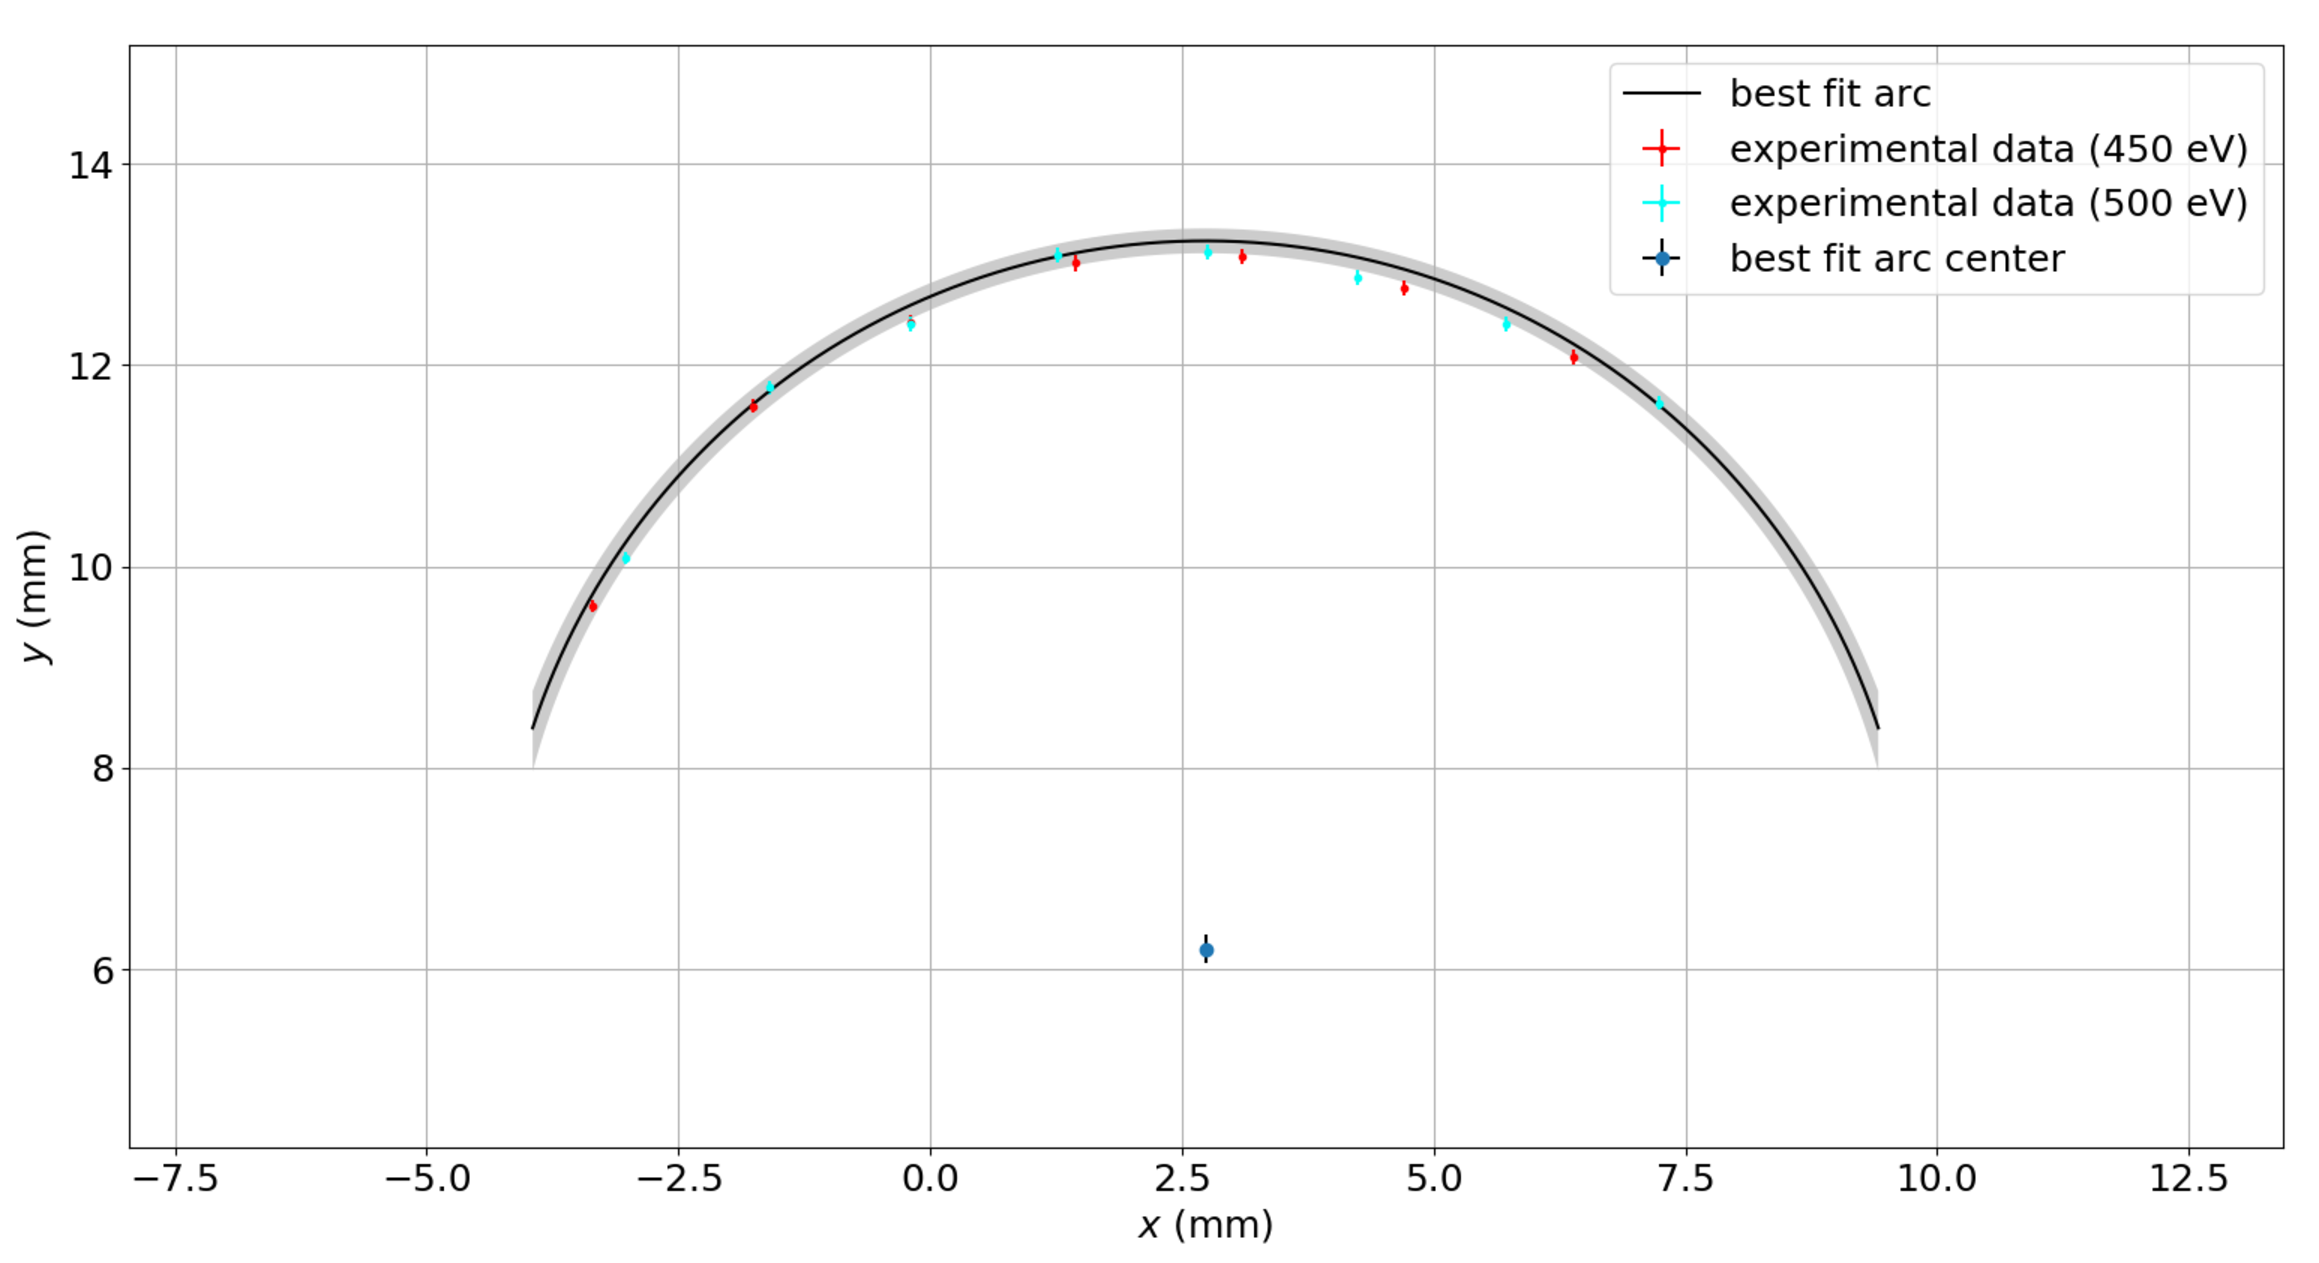
\includegraphics[scale=0.4]{Chapter-3/Figures/arc_fit.pdf}
 \caption[Test-configuration diffracted arc for the TASTE prototype mapped using data gathered at \SI{450}{\electronvolt} and \SI{500}{\electronvolt} fit to a circle]{Test-configuration diffracted arc mapped using data gathered at \SI{450}{\electronvolt} and \SI{500}{\electronvolt} and fit to a circle. Grayed regions represent one standard deviation uncertainty \cite{McCoy20}.}\label{fig:arc_fit_taste}
 \end{figure}
By fitting these data to a half-circle as shown in \cref{fig:arc_fit_taste}, the arc radius was measured as $r = 7.03 \pm \SI{0.12}{\mm}$, and from $r = L \sin \left( \gamma \right)$ [\emph{cf.\@} \cref{eq:arc_radius}], the cone opening half-angle for the diffraction pattern was determined to be $\gamma = 1.73 \pm 0.03^{\circ}$. 

The azimuthal incidence angle, $\alpha$, was measured independently of the roll angle, $\phi$, by \cref{eq:measure_alpha} using $\Delta x_{\text{dir}}$ as the $x$-distance between the direct beam (not shown in \cref{fig:arc_fit_taste}) and the center of the diffracted arc determined from the fit [\emph{cf.\@} \cref{fig:ALS_arc}]. 
With a measured value of $\alpha = 23.4 \pm 0.6^{\circ}$, the roll angle was constrained as $\phi = 1.14 \pm 0.04^{\circ}$ by \cref{eq:measure_roll} using $\Delta x_0$ as the $x$-distance between $0^{\text{th}}$ order and the center of the diffracted arc. 
Using this result and $\Delta y_0$, the $y$-distance between $0^{\text{th}}$ order and the center of the diffracted arc, a graze angle of $\eta \approx 1.5^{\circ}$ was verified through \cref{eq:measure_graze} to give $\eta = 1.56 \pm 0.04^{\circ}$. 
\begin{table}[]
\centering
\caption[Measured parameters for the test-configuration diffracted arc of the TASTE grating prototype at the ALS]{Measured parameters for the test-configuration diffracted arc of the TASTE grating prototype at the ALS \cite{McCoy20}.}\label{tab:arc_params_taste}
\begin{tabular}{@{}ll@{}}
\toprule
parameter                                                                 & measured value             \\ \midrule
system throw ($L$)                                                        & $232.0 \pm 1.4$ mm     \\
arc radius ($r$)                                                          & $7.03 \pm 0.12$ mm       \\
$x$-distance between direct beam and arc center ($\Delta x_{\text{dir}}$) & $2.80 \pm 0.05$ mm       \\
$x$-distance between 0$^{\text{th}}$ order and arc center ($\Delta x_0$)  & $2.92 \pm 0.05$ mm       \\
$y$-distance between 0$^{\text{th}}$ order and arc center ($\Delta y_0$)  & $6.33 \pm 0.14$ mm       \\ \midrule
cone opening half-angle ($\gamma$) by \cref{eq:arc_radius}        	& $1.73 \pm 0.03^{\circ}$  \\
azimuthal incidence angle ($\alpha$) by \cref{eq:measure_alpha}       & $23.4 \pm 0.6^{\circ}$ \\ \midrule
roll (rotation about $z$-axis; $\phi$) by \cref{eq:measure_roll}      & $1.14 \pm 0.04^{\circ}$  \\
graze (rotation about $x$-axis; $\eta$) by \cref{eq:measure_graze}      & $1.56 \pm 0.04^{\circ}$  \\
yaw (rotation about $y$-axis; $\varphi$) by \cref{eq:measure_yaw}     & $0.69 \pm 0.01^{\circ}$  \\ \bottomrule
\end{tabular}
\end{table}
Finally, grating yaw was measured using \cref{eq:measure_yaw} to yield $\varphi = 0.69 \pm 0.01^{\circ}$. 
Summarized in \cref{tab:arc_params_taste}, these measurements indicate a near-Littrow test configuration at $\eta \approx 1.5^{\circ}$ for a blaze angle of $\delta \approx 27^{\circ}$. 

\subsection{Test Results for Diffraction Efficiency}\label{sec:test_results_taste}
%%%%%%%%%%%%%%%%%%%%%%%%%%%%%%%%%%%%%%%%%--------------------------------------------------
In the test geometry established in \cref{sec:grat_geo_taste}, diffraction-efficiency data were gathered as a function of photon energy, $\mathcal{E}_{\gamma}$, where for each measurement, both the diffracted arc and the direct beam were scanned along the $x$-direction in \SI{50}{\um} increments. 
From these measurements, $\mathscr{E}_n$, defined as $\mathcal{I}_n / \mathcal{I}_{\text{inc}}$ [\emph{cf.\@} \cref{eq:diffraction_efficiency}], was calculated according to the methodology described in \cref{sec:measure_efficiency}, with dark current from the photodiode detector taken into account. 
Diffuse scatter arising from surface roughness on the groove facets, which in principle only affects $\mathcal{I}_n$, was estimated using the continuum level in between order maxima and was found to be significant only for $\mathcal{E}_{\gamma} \gtrapprox \SI{600}{\electronvolt}$, where it contributed to $\mathscr{E}_n$ on the level of \SI{1}{\percent} or less for each propagating order. 
These measurements were taken in \SI{20}{\electronvolt} steps, first from \SIrange{440}{800}{\electronvolt} and then from \SIrange{80}{420}{\electronvolt} with the triple-mirror order sorter described in \cref{sec:als_beam}.   

Although the implementation of the order sorter is expected to shift slightly the position of the beam on the grating, and hence the measured parameters listed in \cref{tab:arc_params_taste}, the effect is small and not apparent in the measured absolute efficiency data, which are shown in \cref{fig:abs_eff_taste} compared to $\mathcal{R}_{F}$ for gold at $\zeta = 1.73^{\circ} \approx \gamma$ using \cref{eq:ch3_fres_refl}. 
\begin{figure}
 \centering
 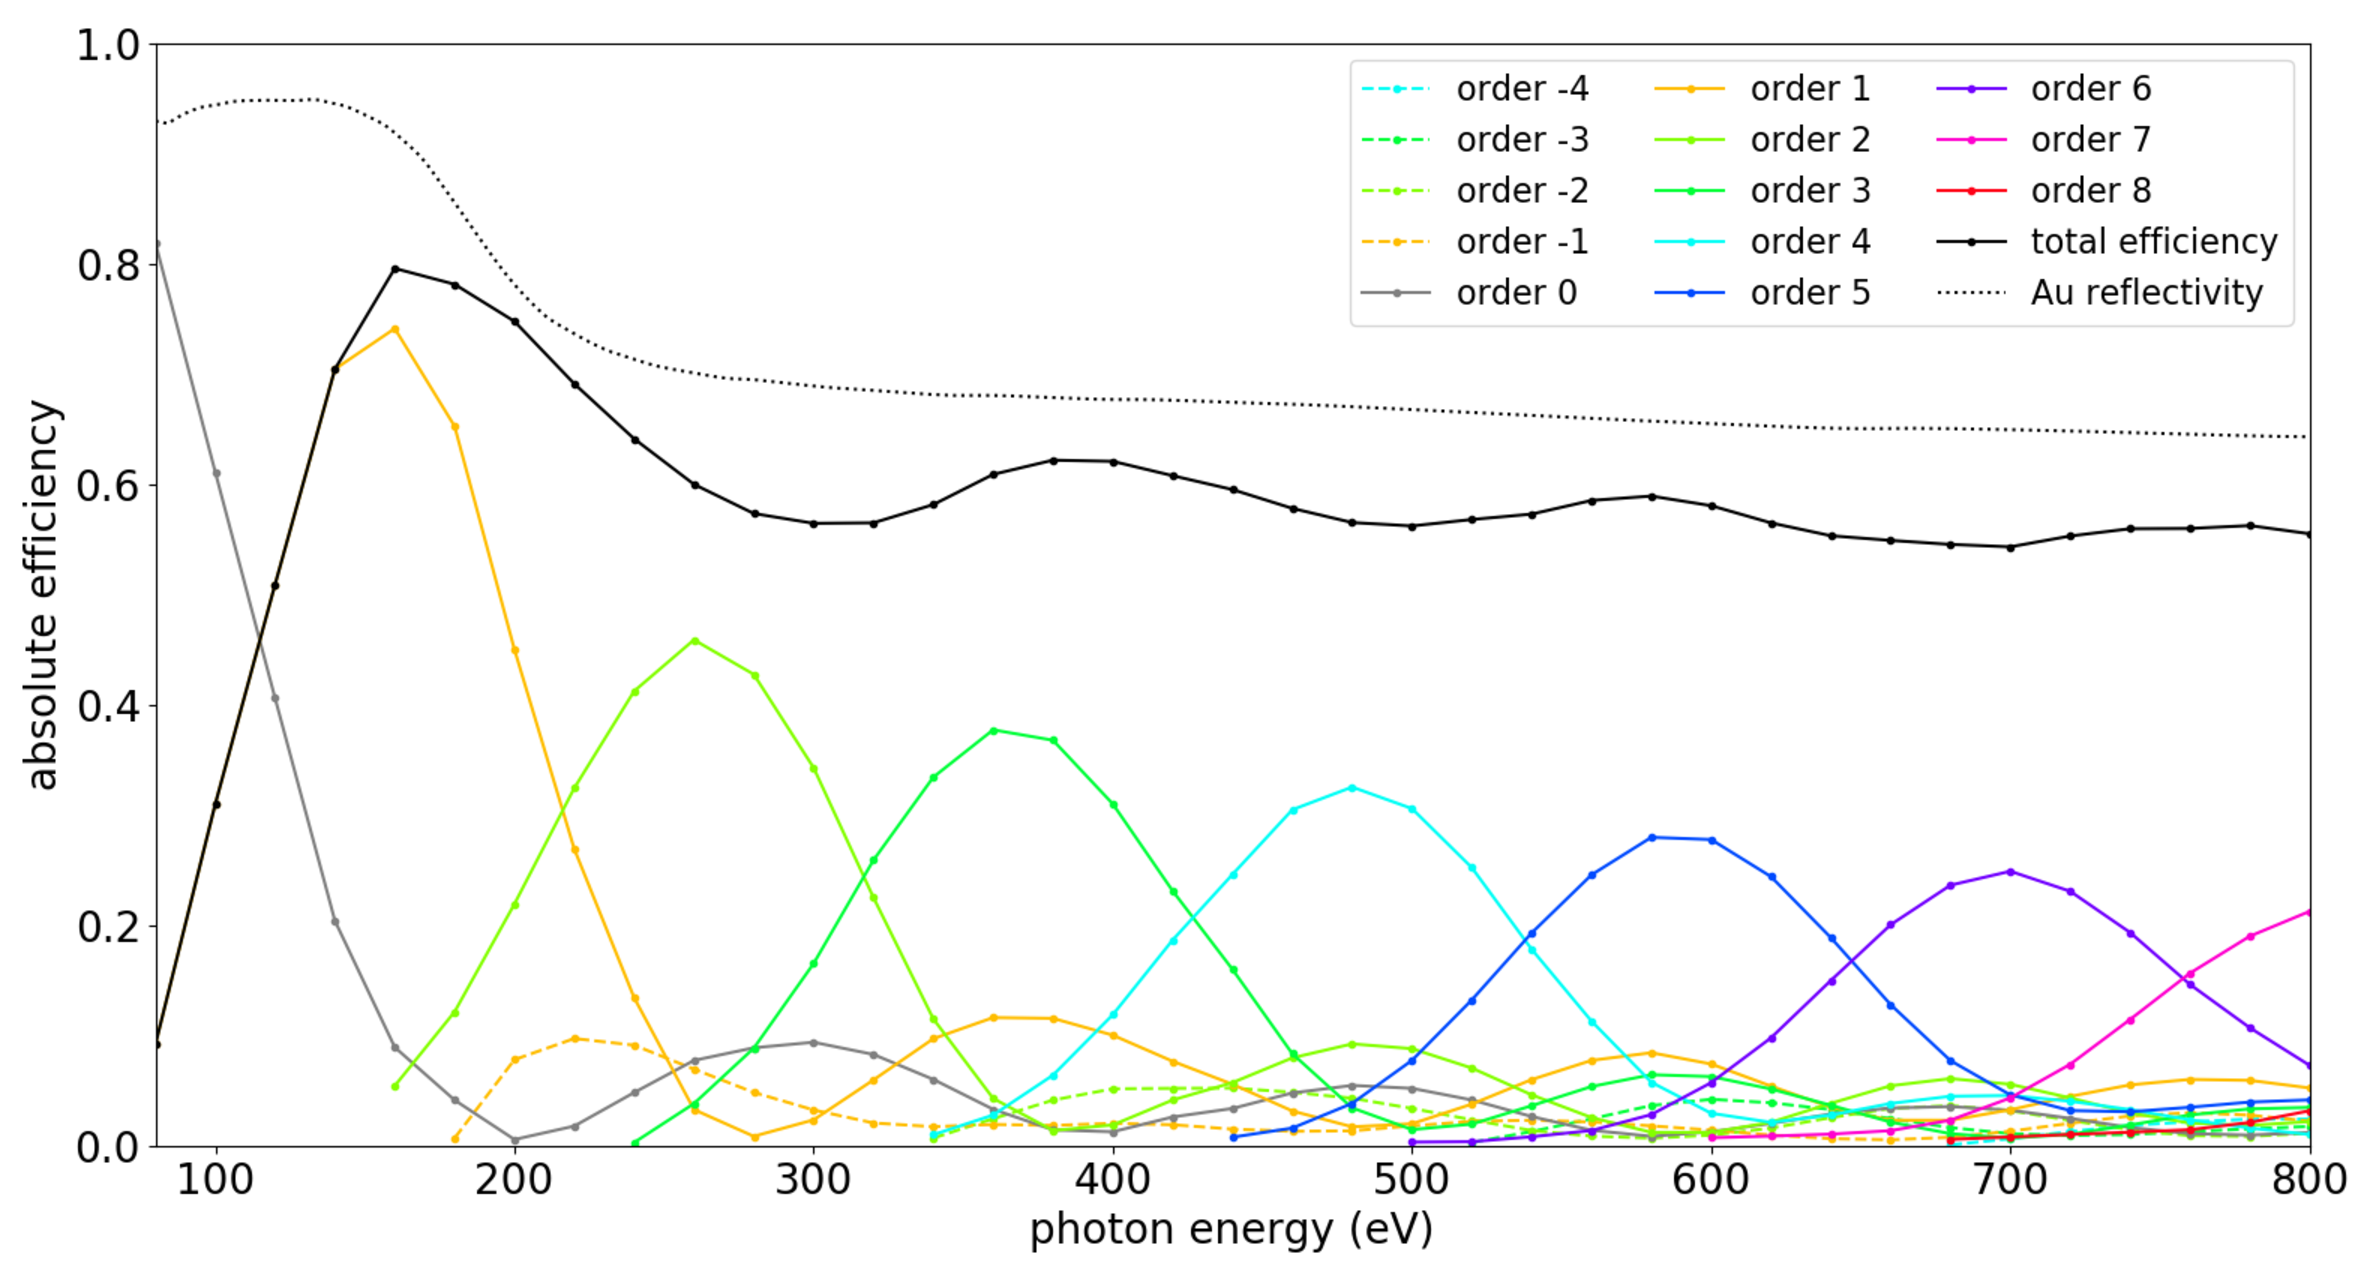
\includegraphics[scale=0.395]{Chapter-3/Figures/absolute_efficiency_data.pdf}
 \caption[Measured absolute diffraction efficiency for the TASTE grating prototype compared to the Fresnel reflectivity of gold]{Data for absolute diffraction efficiency gathered at the ALS compared to the Fresnel reflectivity of gold, $\mathcal{R}_{F}$. Total diffraction efficiency below \SI{240}{\electronvolt} misses contributions from orders $n = \num{2}$ and $n = \num{3}$ on the order of a few percent \cite{McCoy20}.}\label{fig:abs_eff_taste}
 \end{figure} 
However, as indicated most clearly by the sharp cut-off in the measured $n=2$ curve at $\mathcal{E}_{\gamma} \approx \SI{160}{\electronvolt}$, the beam shift evidently caused measurements of propagating orders of $n=\num{2}$ and $n=\num{3}$ with large diffracted angle, $\beta$, to be missed by the photodiode during data collection. 
These data nonetheless show that peak-order efficiency ranges from about \SI{75}{\percent} down to \SI{25}{\percent} as $\mathcal{E}_{\gamma}$, and $n$, increase. 
$\mathscr{E}_{\text{tot}}$, defined as $\sum_n \mathscr{E}_n$ for all propagating orders with $n \neq 0$, is also plotted in \cref{fig:abs_eff_taste} but due to the missing $n=\num{2}$ and $n=\num{3}$ measurements in the EUV, this curve underestimates the true total diffraction efficiency for $\mathcal{E}_{\gamma} < \SI{240}{\electronvolt}$. 
Moreover, relative diffraction efficiency was calculated by dividing each $\mathscr{E}_n$ measurement from \cref{fig:abs_eff_taste} by $\mathcal{R}_{F}$ [\emph{cf.\@} \cref{sec:measure_efficiency}]. 
\begin{figure}
 \centering
 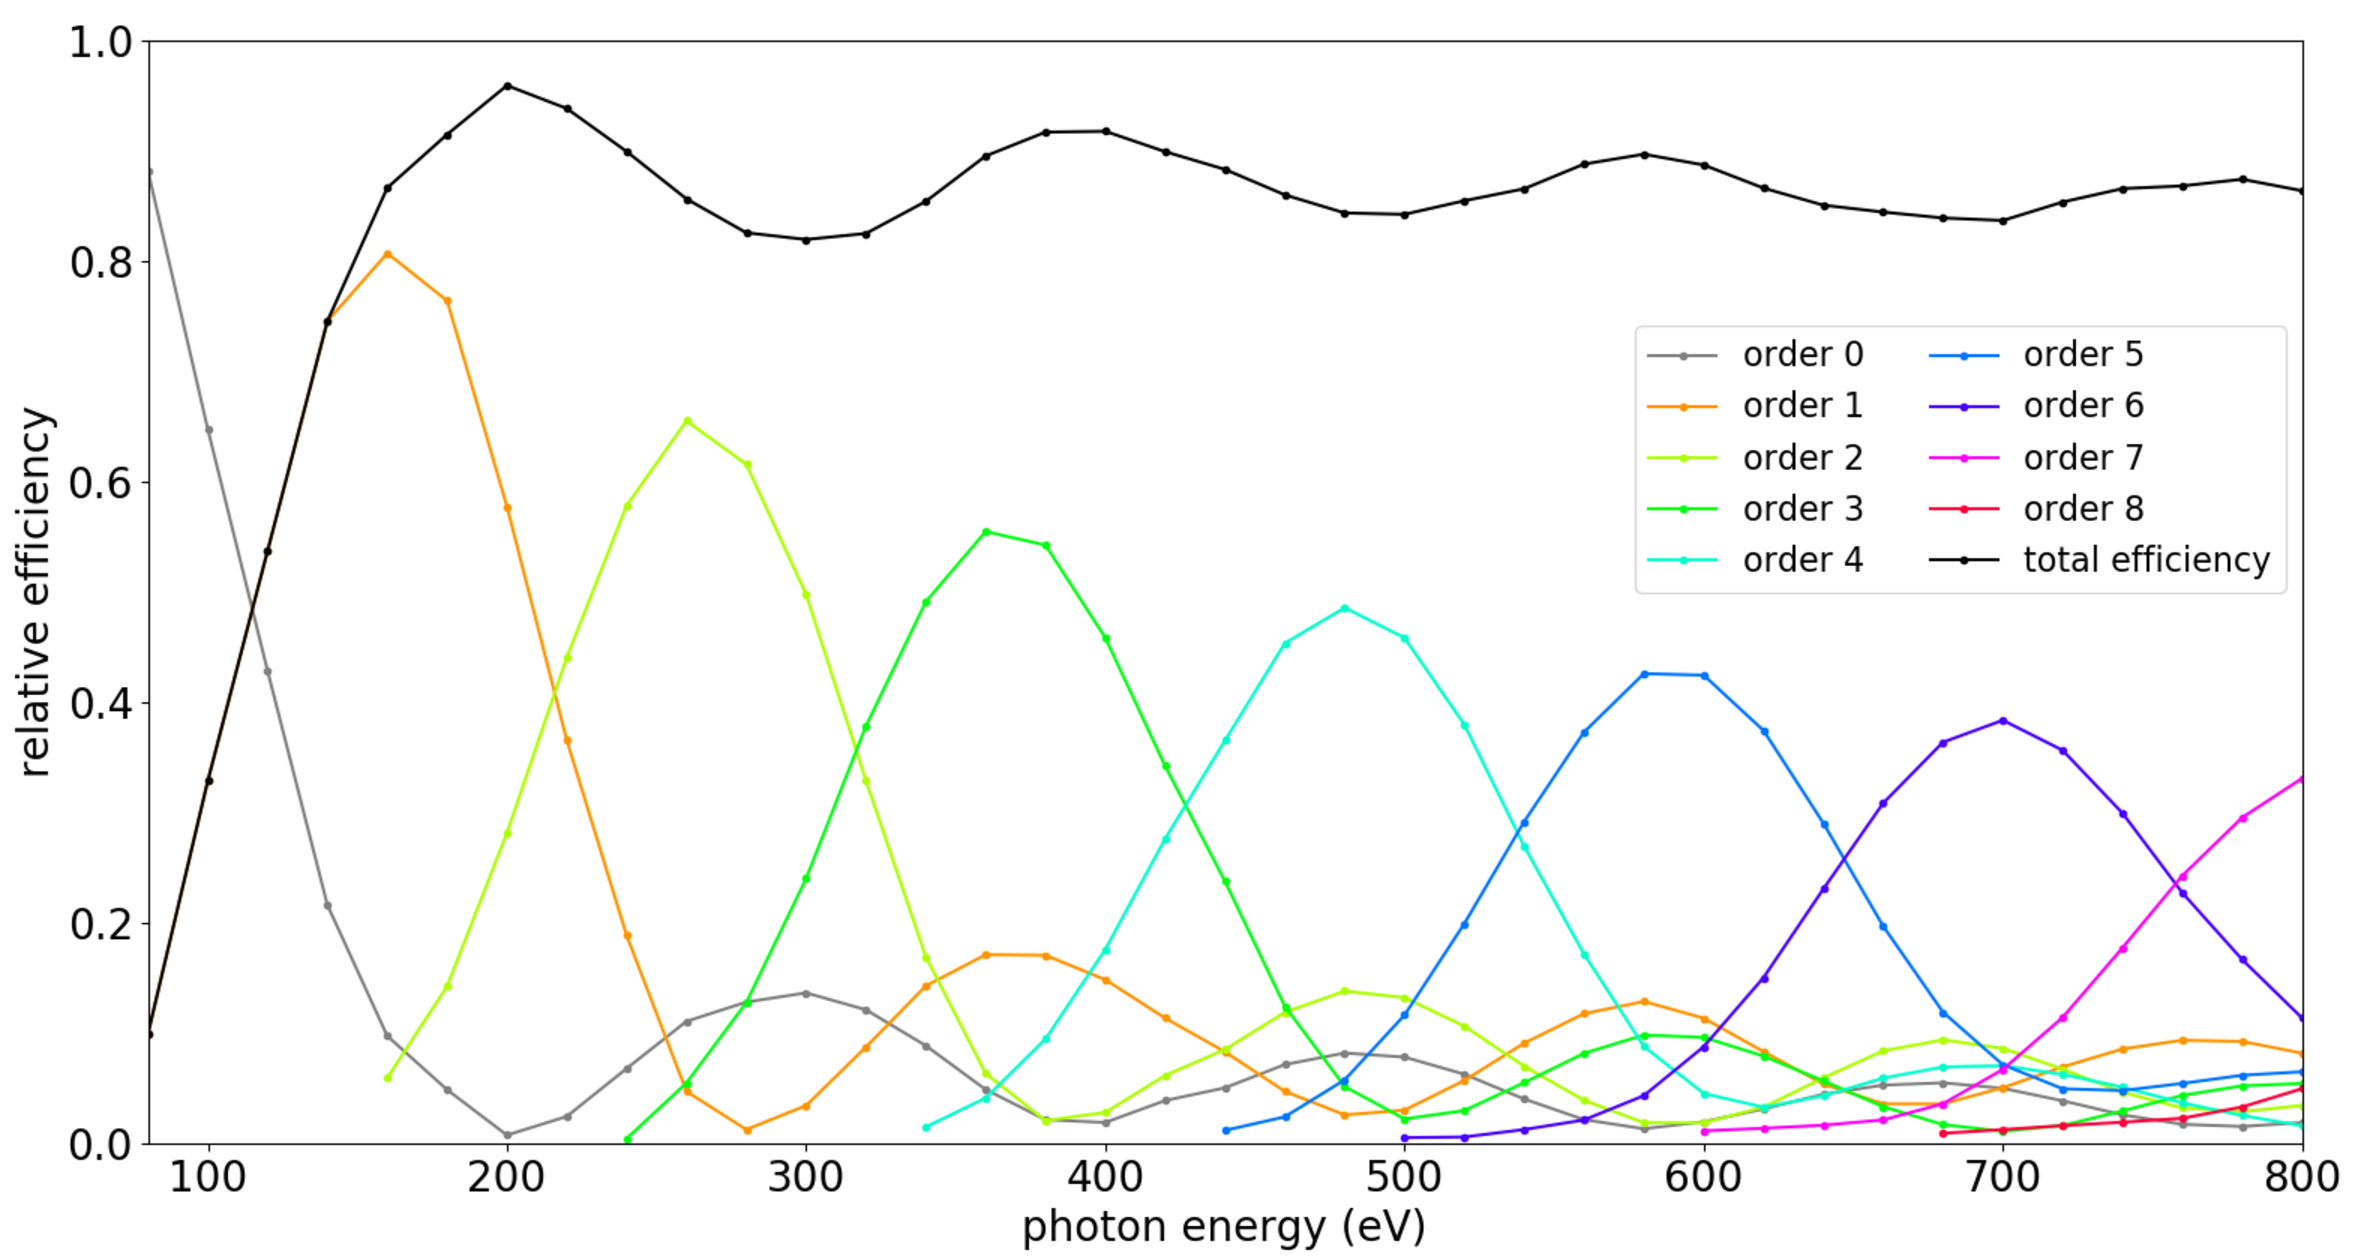
\includegraphics[scale=0.39]{Chapter-3/Figures/relative_efficiency_fix.pdf}
 \caption[Relative diffraction efficiency calculated by dividing absolute diffraction efficiency by the Fresnel reflectivity of gold]{Relative diffraction efficiency calculated by dividing the absolute diffraction efficiency from \cref{fig:abs_eff_taste} by the Fresnel reflectivity of gold, $\mathcal{R}_{F}$. Total relative diffraction efficiency below \SI{240}{\electronvolt} misses contributions from orders $n = \num{2}$ and $n = \num{3}$ on the order of a few percent \cite{McCoy20}.}\label{fig:rel_eff_taste}
 \end{figure}
This result is plotted in \cref{fig:rel_eff_taste}, where total relative diffraction efficiency, $\mathscr{E}_{\text{tot}} / \mathcal{R}_{F}$, ranges from about \SIrange{95}{88}{\percent} as $\mathcal{E}_{\gamma}$ increases from \SIrange{240}{800}{\electronvolt}, where all propagating orders are accounted for [\emph{cf.\@} \cref{tab:eff_benchmark}]. 

\section{Analysis and Discussion}\label{sec:discussion_taste}
%%%%%%%%%%%%%%%%%%%%%%%%%%%%%%%%%%%%%%%%%--------------------------------------------------
The beamline measurements presented in \cref{sec:test_results_taste} indicate that the grating prototype yields an approximate blaze response at EUV and soft x-ray wavelengths in a near-Littrow configuration.  
This is evidenced by the total diffraction efficiency, $\mathscr{E}_{\text{tot}}$, being dominated by single orders with $n > 0$ and peak positions close to those predicted by \cref{eq:blaze_wavelength_TASTE} for the blaze wavelength [\emph{cf.\@} \cref{fig:abs_eff_taste}]. 
However, along with the peak orders that resemble a blaze response, propagating orders of lower $n$ each contribute to $\mathscr{E}_{\text{tot}}$ at a level of $\sim \SI{10}{\percent}$. 
Thus, toward the blue end of the measured bandpass, where a relatively large number of propagating orders exist, peak-order diffraction efficiency is comparatively low and comprises a smaller fraction of $\mathscr{E}_{\text{tot}}$. %exist by \cref{eq:off-plane_orders}
This suggests that diffracted orders gradually become suppressed with increasing $n$ due to an imperfect sawtooth topography generated by the TASTE process outlined in \cref{sec:prototype_TASTE_process}. 
That is, while an ideal blazed grating exhibits a sharp sawtooth topography, the grating prototype features a quasi-flat apex produced by the \SI{100}{\nm}-wide, top staircase step in the GEBL pattern that is nominally unexposed to high-energy electrons and hence largely unaffected by the thermal reflow process. %\footnote{As noted in \cref{sec:reflow_results,sec:prototype_TASTE_process}, however, slight rounding in this top step is thought to have occurred from a degraded reflow selectivity.} 

In addition to an imperfect sawtooth topography, peak-order diffraction efficiency, especially toward the blue end of the spectrum, is impacted by $\lambda$-dependent losses that arise from surface roughness on the groove facets [\emph{cf.\@} \cref{sec:refl_account}]. 
This can be gleaned from analyzing the total relative response from the grating, $\left( \mathscr{E}_{\text{tot}} + \mathscr{E}_0 \right) / \mathcal{R}_{F}$ [\emph{cf.\@} \cref{sec:measure_efficiency}], with $\mathcal{R}_{F}$ given by \cref{eq:ch3_fres_refl}. 
Due to the short, nanoscale penetration depth, $\mathcal{D}_{\perp}$, of gold at grazing incidence [\emph{cf.\@} \cref{fig:Au_refl_attn}], it is justified to treat the grating overcoat material as an infinitely-thick layer of gold using index of refraction data provided by CXRO \cite{CXRO_database}.
The grating's total relative response is plotted in \cref{fig:rough_eff_taste} over $\SI{240}{\electronvolt} \leq \mathcal{E}_{\gamma} \leq \SI{800}{\electronvolt}$, where the data show a monotonic decrease from about \SI{96}{\percent} down to \SI{88}{\percent} as wavelength decreases, suggesting that $\lambda$-dependent losses are occurring. %the range of measured photon energies that include all propagating orders,
\begin{figure}
 \centering
 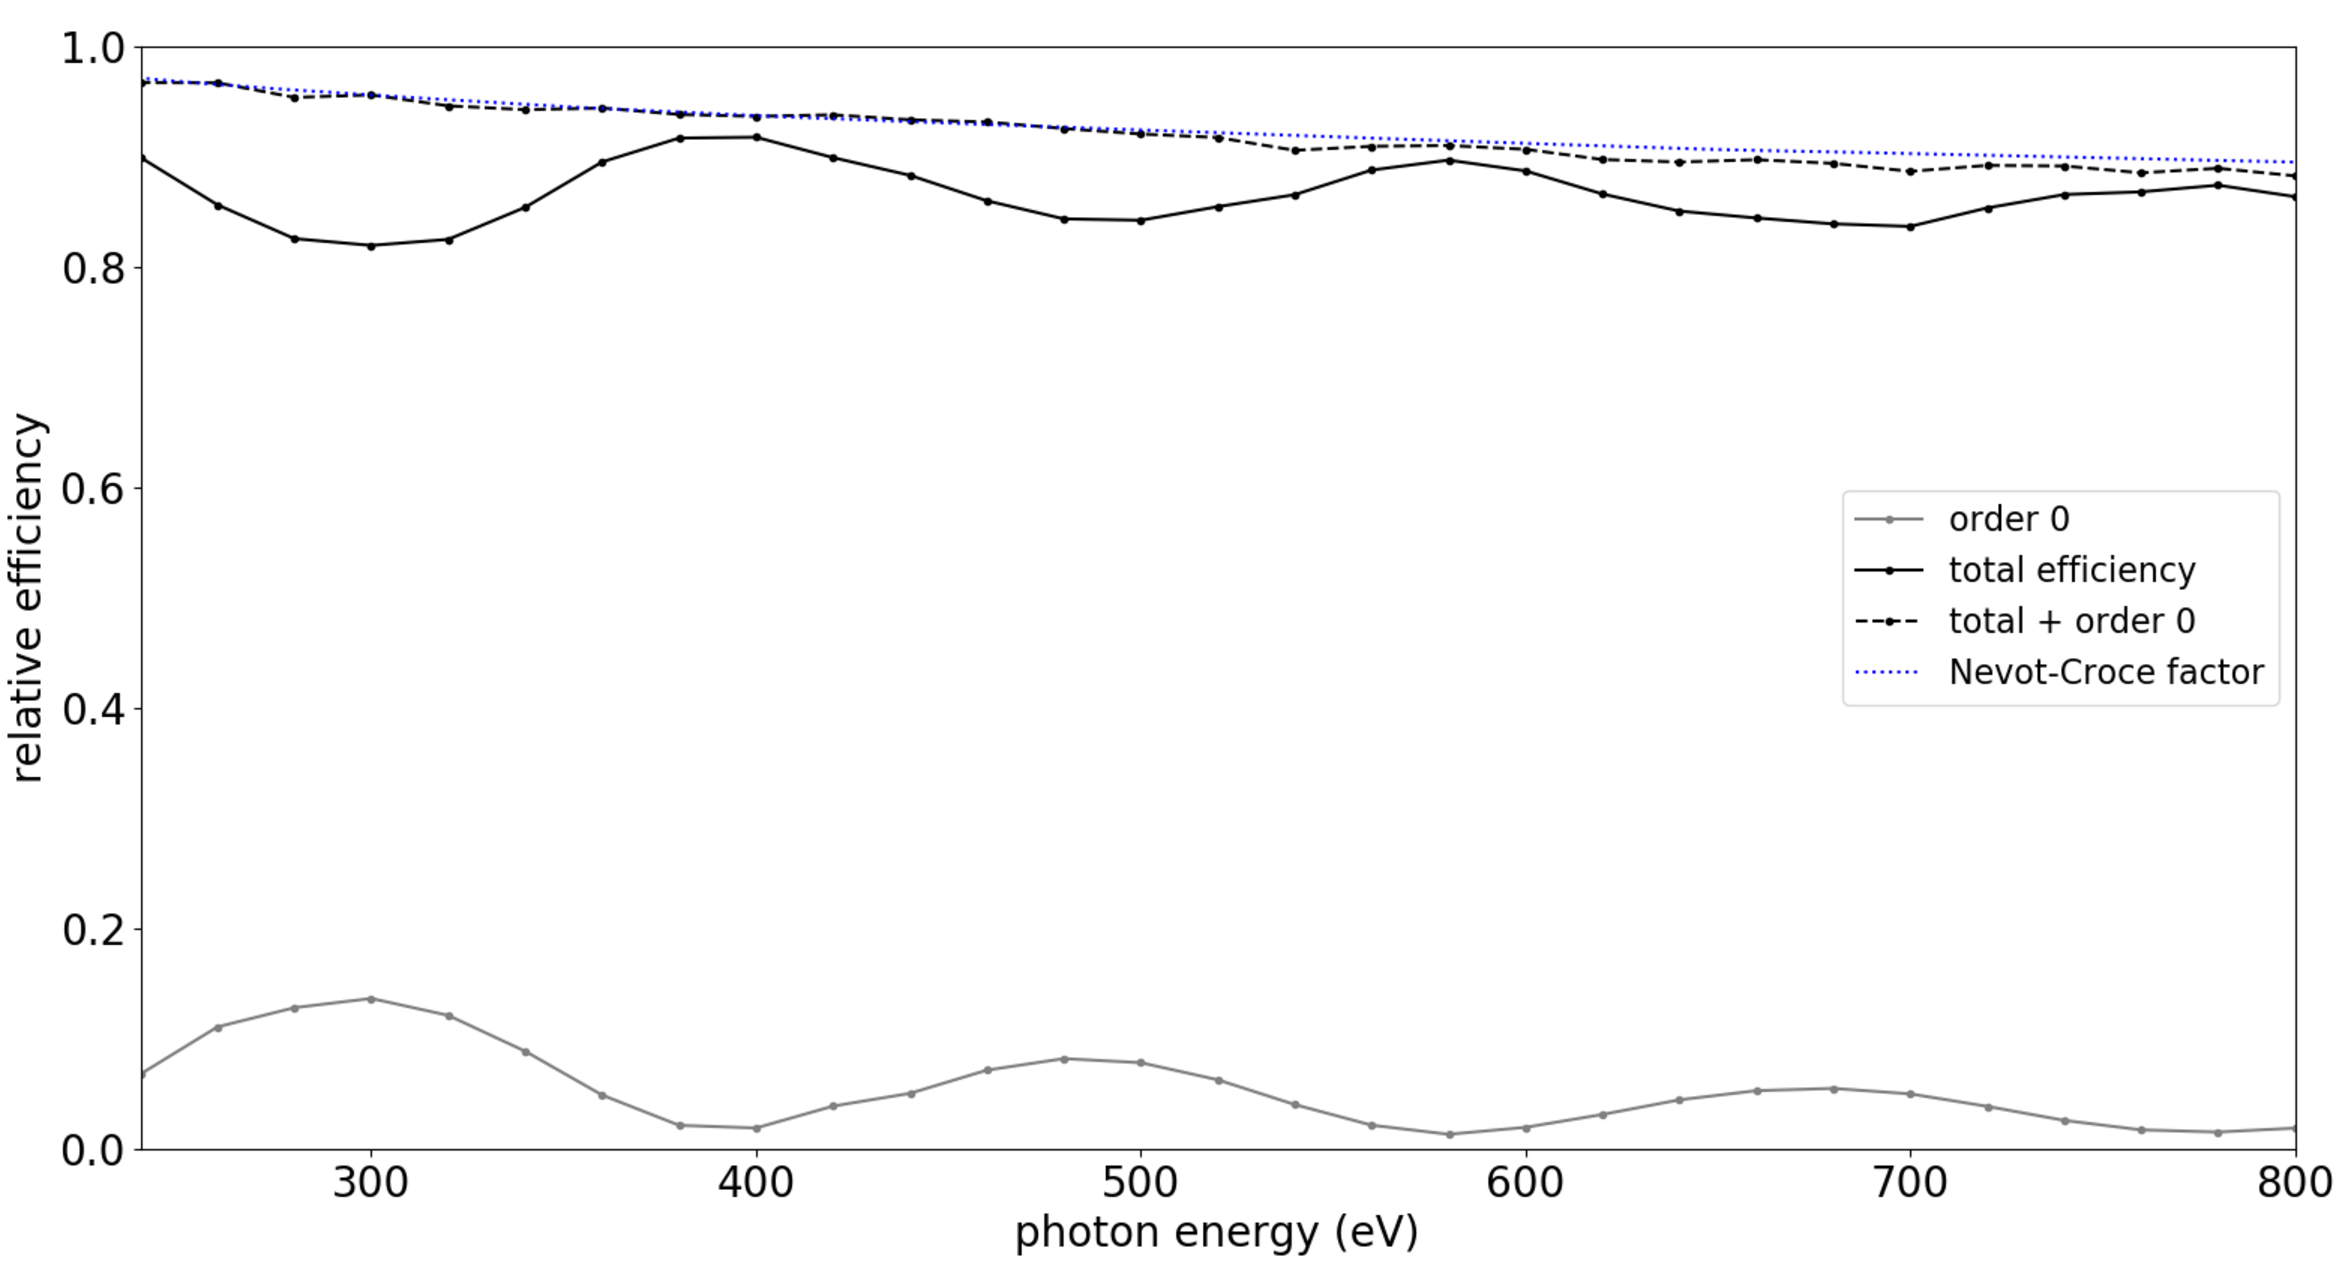
\includegraphics[scale=0.39]{Chapter-3/Figures/total_eff_rough_factor.pdf}
 \caption[Total relative response of the grating prototype, compared to the Nevot-Croce factor]{Total relative response of the grating prototype, defined as the sum of total diffraction efficiency and zero order, relative to the reflectivity of gold. Overlaid is the Nevot-Croce factor [\emph{cf.\@} \cref{eq:nc_factor_taste}] for $\zeta = 1.73^{\circ}$ and $\sigma = \SI{1.5}{\nm}$ RMS, which indicates the theoretical specular reflectivity of a rough surface relative to Fresnel reflectivity, $\mathcal{R}_{F}$ \cite{McCoy20}.}\label{fig:rough_eff_taste}
 \end{figure}
This is to be compared with the specular reflectivity of a hypothetical mirror flat relative to $\mathcal{R}_{F}$ such that its total relative response is \SI{100}{\percent} in the absence of surface roughness. 
In the regime of TER, the reduced specular reflectivity from a rough surface, $\mathcal{R}_{\text{rough}}$, is described approximately by the \emph{Nevot-Croce factor} [\emph{cf.\@} \cref{sec:refl_account}]. 
For a thick slab of gold with a complex index of refraction $\tilde{\nu} (\omega)$, a grazing-incidence angle $\zeta$ and RMS surface roughness $\sigma$, the norm-squared of this factor is given by \cref{eq:NC_refl_ratio} with $\mathcal{R}_{NC} = \mathcal{R}_{\text{rough}}$:
\begin{equation}\label{eq:nc_factor_taste}
  \frac{\mathcal{R}_{NC}}{\mathcal{R}_F} = \norm{\mathrm{e}^{- 2 k_{\perp} \tilde{k}_{\perp} \sigma^2}}^2 = \mathrm{e}^{-4 k_0^2 \sin \left( \zeta \right) \Re \left[ \sqrt{\tilde{\nu}^2 (\omega) - \cos^2 \left( \zeta \right) } \right] \sigma^2} ,
 \end{equation}
where $k_{\perp} = - k_0 \sin \left( \zeta \right)$ and $\tilde{k}_{\perp} = -k_0 \sqrt{\tilde{\nu}^2 (\omega) - \cos^2 \left( \zeta \right)}$ are the components of the wave vector normal to the surface in vacuum and gold, respectively, with $k_0 \equiv 2 \pi / \lambda$. 
Moreover, $\Re \left[ \sqrt{\tilde{\nu}^2 (\omega) - \cos^2 \left( \zeta \right) } \right]$ represents the real part of $-\tilde{k}_{\perp} / k_0$. 

As described in \cref{sec:refl_account}, the Nevot-Croce factor defined by \cref{eq:nc_factor_taste} is valid for small roughness features taking on a Gaussian height distribution with $\abs{k_{\perp}} \sigma \ll 1$ so that using $\sigma \approx \SI{1.5}{\nm}$ RMS as measured by AFM and $\zeta = 1.73^{\circ}$, this condition is satisfied for  
\begin{equation}\label{eq:rough_condition}
 \lambda \gg 2 \pi \sigma \sin \left( \zeta \right) \approx \SI{0.3}{\nm}  .
 \end{equation}
Additionally, derivations of the Nevot-Croce factor assume a very small surface correlation length, $\ell_{\text{corr}}$ [\emph{cf.\@} \cref{eq:auto_correlation_normal}], that satisfies $\ell_{\text{corr}} k^2_{\perp} \ll k_0$ \cite{deBoer95}. 
Keeping $\ell_{\text{corr}}$, which represents the lateral size scale of roughness features, as an unknown, this yields 
\begin{equation}\label{eq:corr_condition}
 \lambda \gg 2 \pi \ell_{\text{corr}} \sin^2 \left( \zeta \right) \approx 0.006 \ell_{\text{corr}} . 
 \end{equation}
If \cref{eq:rough_condition,eq:corr_condition} are fulfilled, diffuse scatter in vacuum can in principle be neglected and $\lambda$-dependent losses attributed to absorption as radiation scatters into the medium. 
Otherwise, radiation of wavelength $\lambda$ is able to diffract from roughness spatial frequencies on the order of $\ell_{\text{corr}}^{-1}$, producing diffuse scatter that can be detected by the photodiode, in which case details of the \emph{power spectral density (PSD) function} for surface roughness [\emph{cf.\@} \cref{eq:PSD_general}] are required to obtain a more accurate expression for $\mathcal{R}_{\text{rough}}$ \cite{deBoer95,Wen15}. 

Because the PSD function for surface roughness is not known for the groove facets on the grating prototype, \cref{eq:nc_factor_taste} was taken to approximate $\left( \mathscr{E}_{\text{tot}} + \mathscr{E}_0 \right) / \mathcal{R}_{F}$ for the grating prototype in the presence of surface roughness. 
This is plotted in \cref{fig:rough_eff_taste}, where it is seen that the data closely match the Nevot-Croce factor with the experimentally-determined values of $\zeta \approx \gamma = 1.73^{\circ}$ and $\sigma \approx \SI{1.5}{\nm}$ RMS. 
This supports the idea that absorption due to surface roughness on the groove facets is responsible for the losses in the grating's total response over $\SI{240}{\electronvolt} \leq \mathcal{E}_{\gamma} \leq \SI{800}{\electronvolt}$.  %the measured bandpass that encompasses all propagating orders. 
Although the detection of diffuse scatter for $\mathcal{E}_{\gamma} \gtrapprox \SI{600}{\electronvolt}$ ($\lambda \lessapprox \SI{2}{\nm}$) [\emph{cf.\@} \cref{sec:taste_eff_results}] suggests that the conditions for the Nevot-Croce factor to be valid are not strictly fulfilled at these relatively short wavelengths, \cref{fig:rough_eff_taste} indicates that \cref{eq:nc_factor_taste} is a decent approximation across the bandpass considered.
However, future diffraction efficiency test campaigns should better quantify diffuse scatter due to surface roughness in a similar manner to x-ray reflectivity experiments that aim to characterize surfaces, materials and inter-facial roughness \cite{Gay1999,Baumbach1999}. 

To investigate the impact that an imperfect sawtooth topography with an unpointed apex has on the measured diffraction efficiency, data for $\mathscr{E}_n$ were modeled according to the vector diffraction theory framework outlined in \cref{sec:integral_method}. 
This was handled using the software package \textsc{PCGrate-SX} (v.\ 6.1) \cite{PCGrate_web}, which solves the Helmholtz equation through the integral method for a custom grating boundary and incidence angles input by the user \cite[\emph{cf.\@} \cref{sec:grat_bound_consider}]{Goray10}. 
Previous beamline experiments have verified a lack of polarization sensitivity for x-ray reflection gratings used in extreme off-plane mounts \cite{Marlowe16} and as a result, \textsc{PCGrate-SX} calculations were carried out assuming a perfectly conducting grating boundary with perfectly smooth groove facets and an incident wavefront with \emph{TE polarization} [\emph{cf.\@} \cref{fig:polarization_angle,sec:dirch_bound}].  
Although perfect conductivity combined with the absence of surface roughness implies a lossless response from the grating grooves [\emph{cf.\@} \cref{sec:rel_eff_perf}], \textsc{PCGrate-SX} modulates the predicted diffraction efficiency by the reflectivity of a user-input, stratified medium defined by index of refraction data and custom layer thicknesses [\emph{cf.\@} \cref{sec:refl_account}]. 

Taking the grating material to be an infinitely-thick layer of gold as discussed above, the cross-sectional groove shape of the grating prototype was approximated as an acute trapezoid with a near-vertical lateral side opposite a slope that emulates the active blaze facet. 
Additionally, a flat bottom portion was included to represent the cleared portion of the resist described in \cref{sec:TASTE_prototype}. 
\begin{figure}
 \centering
 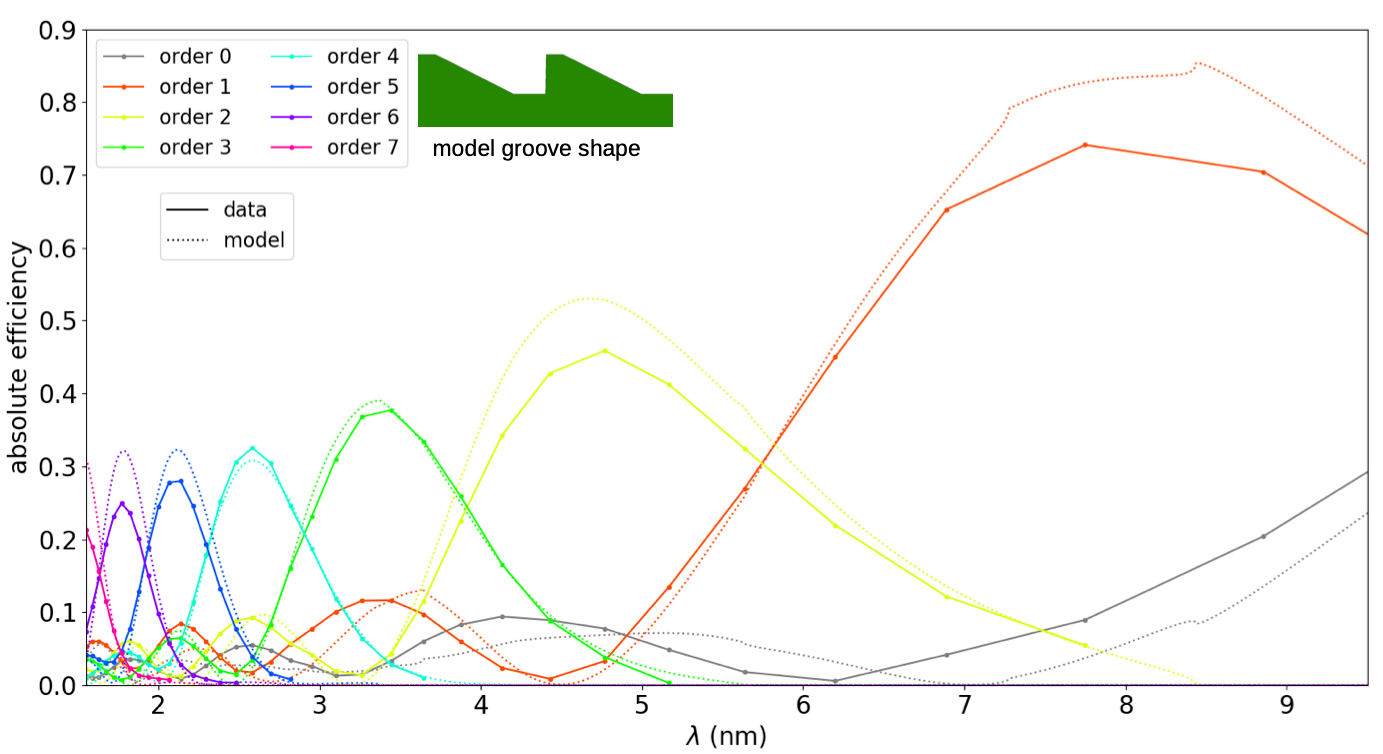
\includegraphics[scale=0.65]{Chapter-3/Figures/absolute_efficiency_model_wav.pdf} %85 nm land, 120 nm depth, 77 nm ridge, 27 blaze angle, 89 steep angle
 \caption[Measured absolute diffraction efficiency compared to theoretical diffraction efficiency modeled using \textsc{PCGrate-SX}]{Absolute diffraction efficiency from \cref{fig:abs_eff_taste} compared to theoretical diffraction efficiency modeled using \textsc{PCGrate-SX}. Modeled data are multiplied by the Nevot-Croce factor [\emph{cf.\@} \cref{eq:nc_factor_taste}] for $\zeta = 1.73^{\circ}$ and $\sigma = \SI{1.5}{\nm}$ RMS \cite{McCoy20}.}\label{fig:model_eff_taste}
 \end{figure}
Using the nominal values of $\alpha$ and $\gamma$ listed in \cref{tab:arc_params_taste} for grating incidence angles and $d = \SI{400}{\nm}$ for the groove spacing, a series of \textsc{PCGrate-SX} calculations were performed for a range of trapezoids with slightly-varying dimensions close to those measured by AFM in \cref{fig:coating_AFM}. 
The model matching the measured data most closely was one with a blaze angle of $\delta = 27^{\circ}$, a groove depth of \SI{120}{\nm}, a flat-top width of \SI{77}{\nm} and bottom-width of \SI{85}{\nm}. 
These predicted data, modulated by the Nevot-Croce factor from \cref{fig:rough_eff_taste}, are plotted as a function of $\lambda$ in \cref{fig:model_eff_taste} and compared to $\mathscr{E}_n$ measured for orders $n=0$ through $n=7$. 

It is seen in \cref{fig:model_eff_taste} that the measured peak-order positions match roughly those predicted by the model, demonstrating that the grating prototype has an efficiency response similar to that of a blazed grating with $d=\SI{400}{\nm}$~ and $\delta = 27^{\circ}$ at the experimentally-determined incidence angles of $\alpha = 23.4^{\circ}$ and $\gamma = 1.73^{\circ}$. 
However, the amplitudes of the peak orders generally fall short of the model with the apparent exceptions of $n=3$ and $n=4$. 
This phenomenon seems to be due in part to the mismatches that exist between the measured data and the model for secondary diffraction peaks, suggesting that the groove shape trapezoidal approximation is not sufficient to reproduce these results to a high degree of accuracy. 
The grating prototype grooves likely have an apex that is slightly rounded as a result of the thermal reflow process but this is difficult to verify through AFM because the shape of the \textsc{SCANASYST-AIR} tip is convolved with the true grating topography in the micrographs shown in \cref{fig:TASTE_AFMs,fig:coating_AFM}. 
Nonetheless, rounding of corners or other deviations from an ideal acute trapezoid are expected to have an impact on the distribution of diffraction efficiency among orders. 
It is also seen in \cref{fig:model_eff_taste} that measured peak-order efficiency becomes increasingly diminished relative to the model as order number increases beyond $n=4$, which is consistent with the observation already mentioned that the relatively large number of orders at short $\lambda$ each contribute substantially to $\mathscr{E}_{\text{tot}}$ while the peak order comprises a relatively smaller fraction. 
This is another indication of there being groove-shape imperfections that diminish the grating prototype's blaze response. 
A possible explanation beyond rounded corners at the apex is irregularity or non-flatness of the sloped surfaces of the grating grooves across the prototype. 
In principle, this could be caused in part by a non-uniform spin-coat thickness but it is expected that the imperfect blazed grating topography produced by TASTE process described in \cref{sec:prototype_TASTE_process} is the largest contributor to this issue.  

\section{Summary and Conclusions}\label{sec:ch3summary}
%%%%%%%%%%%%%%%%%%%%%%%%%%%%%%%%%%%%%%%%%--------------------------------------------------
A prototype for a reflection grating with a groove spacing of \SI{400}{\nm} was fabricated by generating an approximate sawtooth topography in \SI{130}{\nm}-thick PMMA resist coated on a silicon wafer using the TASTE process established in \cref{sec:TASTE} and then coating the grating grooves with a thin layer of gold via EBPVD for reflectivity, using titanium for adhesion. %at the Penn State Materials Research Institute
Diffraction-efficiency measurements gathered at beamline 6.3.2 of the ALS \cite{ALS_632,Underwood96,Gullikson01}, which span $\SI{15.5}{\nm} \gtrapprox \lambda \gtrapprox \SI{1.55}{\nm}$ in a grazing incidence, extreme off-plane mount, demonstrate that the prototype behaves approximately as a blazed grating with $\delta \approx 27^{\circ}$. % groove cross-sections shaped like an acute trapezoid and a blaze angle of $\delta \approx 27^{\circ}$. 
The total response from the grating relative to the reflectivity of the gold overcoat measures between \SIlist{96;88}{\percent} in the soft x-ray, with losses attributed to absorption and diffuse scatter from grating facets with $\sim \SI{1.5}{\nm}$ RMS surface roughness. 
However, even with losses accounted for, the blaze response is observed to diminish for peak orders with $n \geq 5$. 
While this phenomenon is a result of the TASTE process yielding an imperfect sawtooth topography, these results show that TASTE is a promising fabrication technique for the manufacture of custom reflection gratings for soft x-ray spectroscopy \cite{McCoy18,McCoy20}.

An especially important feature of the TASTE process is its ability to define a sawtooth-like topography over a groove layout defined by EBL while also avoiding the dependences on crystallographic structure that exist in processes that \ce{KOH} etching to provide a grating blaze \cite{Franke97,Chang03,McEntaffer13,Miles18}. 
This is particularly advantageous for realizing fanned, curved or other variable-line-space groove layouts that are required for achieving high $\mathscr{R} = \lambda / \Delta \lambda$ while also having blazed groove facets that enable high spectral sensitivity. %also, possibly curved substrates
With $\mathscr{E}_{\text{tot}}$ exceeding \SI{40}{\percent} in the soft x-ray bandpass, these results show that gratings fabricated by TASTE are capable of meeting \emph{Lynx} requirements in terms of spectral sensitivity [\emph{cf.\@} \cref{tab:eff_benchmark}]. 
Additionally, an absolute efficiency of \SI{75}{\percent} in $n=1$ at $\mathcal{E}_{\gamma} \approx \SI{160}{\electronvolt}$ gives an indication that TASTE can realize a highly-efficient grating for EUV spectroscopy with modification of grating parameters. 
However, further work in nanofabrication and beamline testing for $\mathscr{R}$ is required to determine to what degree TASTE is able to make improvements in these areas of technological development. 
In particular, producing gratings with groove spacing significantly smaller than \SI{400}{\nm} that maintain a satisfactory sawtooth topography is challenging from the standpoint of fabrication by TASTE \cite{McCurdy20}; this is discussed further in \cref{ch:conclusions}. 